\documentclass[a4paper, 12pt, openany, oneside, english, brazil]{scrbook} %Classe scrbook do Koma-Script
% para impressão física você pode considerar a troca de oneside para twoside
% \documentclass[a4paper, 12pt, openany, oneside, english, brazil]{scrbook} %Classe scrbook do Koma-Script

%Muda estilo da fonte usada nos títulos dos capítulos, seções e listas para a fonte usada no texto.
\addtokomafont{disposition}{\rmfamily}

%Pacote que permite evitar o erro "No room for new \write" enviando todas as escritas artravés do arquivo .aux
\usepackage{scrwfile}


%Pacotes para apêndices
\usepackage[toc,page]{appendix}


%Pacotes de linguagens, codificação de caracteres e tipografia
%Provê suporte para tipografia em várias línguas
\usepackage[brazil]{babel} % Confirme se o pacote babel-portuges está instalado.


%Pacotes de codificação e fontes
\usepackage[utf8]{inputenc} %Traduz codificações de entrada para a linguagem interna do LaTeX
%\usepackage[latin1]{inputenc}
\usepackage[T1]{fontenc}
\usepackage{fontawesome}
\usepackage{dsfont}
\usepackage{cmap}
\usepackage{lmodern}


%Pacotes de Referências
%Pacote de referências bilbiográficas
\usepackage[bibstyle=authoryear, citestyle=authoryear, maxcitenames=3, maxbibnames=20, hyperref=true, backref=true, backrefstyle=three]{biblatex} % Permite customizar citações. Mais moderno que natbib e bibtex.
%\DefineBibliographyStrings{english}{%
%	backrefpage = {page},% originally "cited on page"
%	backrefpages = {pages},% originally "cited on pages"
%}

%Pacotes de glossários e índices 

%Pacote usado para gerar índice remissivo
%Carregado antes do pacote hyperlink para que funcionem juntos
\usepackage{imakeidx}

%É preferível carregar hyperref após o biblatex, caso esteja usando-o, mas antes do glossaries!
%\usepackage[colorlinks, hyperindex, plainpages=false, pdfusetitle, pdflang=en]{hyperref}
\usepackage[colorlinks, hyperindex, plainpages=false, pdfusetitle, pdflang=pt-BR]{hyperref}

\usepackage[automake, acronym, toc]{glossaries}
%\usepackage[savewrites, nomain, acronym]{glossaries-extra} %Gerando conflito com book mas não com scrbook. Tem que instalar os módulos das linguagens a serem utilizadas. Opção nomain indica que o índice remissivo não será usado. A escolha é sua. Só tenha cuidado com o erro "No room for a new \write. \end{document}", quando o LaTeX tem muitos arquivos auxiliares abertos. A opção "savewrites" usa só um write para todos os arquivos auxiliares do glossaries, mas pode gerar problemas de referências com localizações erradas. Erro corrigido usando o pacote scrwfile



%Pacotes diversos
\usepackage{adjustbox}
\usepackage{indentfirst} % paragrafo na primeira linha escrita
\usepackage{url} %Permite quebras de linhas em certos caracteres ou combinações de caracteres
\usepackage{microtype} %Permite que se façam melhorias de justificação
\usepackage{enumitem} %Permite um maior controle sobre os layouts dos ambientes enumerate, itemize e description
\usepackage{pdflscape} %Permite que páginas sejam exibidas em formato landscape
\usepackage{hologo}%Pacote que define glifos de logos associados com TeX


%Pacotes matemáticos
\usepackage{mathtools} %Carrega automaticamente o amsmath
\usepackage{amssymb} %Pacotes da AMS (American Mathematical Society) para representação de símbolos e equações
\usepackage{esvect} %Provê estilos diferentes para setas que denotam vetores
\usepackage{siunitx} %Provê definições por nome e espaçamentos padrões para unidades padrão
\usepackage{bussproofs} %Permite criar árvores de provas no estilo de cálculo sequente
\usepackage{lplfitch} %Esses dois comandos abaixo são necessários  para que o pacote lplfitch funcione com os pacotes KOMA.
\DeclareOldFontCommand{\sf}{\normalfont\sffamily}{\mathsf}
\DeclareOldFontCommand{\bf}{\normalfont\bfseries}{\mathbf}
\usepackage{natded} %Provê comandos para mostrar provas no estilos usados por Jaśkowski e Kalish e Montague
\usepackage{zed-csp} %Suporta especificações em CSP e Z
%\usepackage{circus} %Define comandos para realizar especificações em circus


%Pacotes de objetos float e cores
%\usepackage{multirow} %Cria células que se estendem por várias linhas em ambientes tabulares 
\usepackage{graphicx} %Incluído com opção dvipdfm para eliminar erro que diz que não pode determinar tamanho de imagem. Essa opção elimina as figuras do texto!!!
\usepackage{colortbl} %Permite adicionar cores a tabelas em LaTeX
% Pacote para o uso de algoritmos
\usepackage[algochapter, linesnumbered, lined, portuguese, ruled]{algorithm2e} %Implementa o environment algorithm
\usepackage{subfig} %Permite a definição de sub-figuras
\usepackage{float} %Provê uma interface melhorada para objetos float
\usepackage{bm} %Define o comando \bm que torna seu argumento em negrito
\usepackage{setspace} %Permite ajustar facilmente espaçamento entre linhas
\usepackage{multirow} %Permite a utilização de multilinhas e multicolunas em ambientes tabulares
\usepackage[x11names]{xcolor} %Pacote que define cores de vários modelos com nomes
\usepackage[chapter]{minted} %Pacote que permite a configuração fácil de código a ser mostrado. A opção chapter realiza a numeração por capítulo
\renewcommand{\listingscaption}{Código}
\renewcommand{\listoflistingscaption}{Lista de Códigos}


%Pacotes para gerar desenhos e animações
\usepackage{qtree} %Permite desenhar diagramas de árvores
\usepackage{pgf} %Permite criar desenhos independentes de plataforma e formato, gerando saída em PS ou PDF
\usepackage{tikz} %Pacote usado para criar gráficos, figuras e ilustrações
\usepackage[tikz]{bclogo} %Permite colorir caixas virtuais ao redor de textos
\usepackage{tikz-dependency} %Provê uma bilbioteca para desenhar grafos de dependência
\usepackage{tikz-network} %Provê uma bilbioteca para desenhar redes complexas
\usepackage{tikz-3dplot} %Permite definir sistemas de coordenadas 3D para desenhar em 3D
\usetikzlibrary{switching-architectures} %Permite desenhar arquiteturas de comutação
\usetikzlibrary{mindmap} %Permite desenhar mapas mentais
\usetikzlibrary{decorations.fractals} %Permite desenhar fractais do tipo curva monstro
\usepackage{pgfplots}%Permite criar plots normais/logaritmicos em 2D/3D
\pgfplotsset{width=7cm,compat=1.17}
\pgfdeclarelayer{background} %Definição necessárias para alguns comandos TikZ
\pgfdeclarelayer{foreground} %Definição necessárias para alguns comandos TikZ
\pgfsetlayers{background, main, foreground} %some additional layers for demo
\usepackage{forest}%Permite desenhar árvores
\definecolor{folderbg}{RGB}{124,166,198}
\definecolor{folderborder}{RGB}{110,144,169}
\definecolor{bgblue}{RGB}{187,222,251}
\definecolor{bggray}{RGB}{220,220,100}

%Definições usadas para gerar desenhos de arquivos em uma ilustração de uma estrutura de árvore que não uso mais 
\def\Size{4pt}
\tikzset{
	folder/.pic={
		\filldraw[draw=folderborder,top color=folderbg!50,bottom color=folderbg]
		(-1.05*\Size,0.2\Size+5pt) rectangle ++(.75*\Size,-0.2\Size-5pt);  
		\filldraw[draw=folderborder,top color=folderbg!50,bottom color=folderbg]
		(-1.15*\Size,-\Size) rectangle (1.15*\Size,\Size);
	}
}

%Pacotes de comentários e mudanças
% Margem aumentada para receber comentários sem reclamar muito
\setlength{\marginparwidth}{2cm}
%%%%%%%%%%%%%%%%%%%%%%%%%%%%%%%%%%%%%%%%%%%%%%%%%%%%%%%%%%%%%%%%%%%
%%
%% Packages for tracking changes
%%
%%%%%%%%%%%%%%%%%%%%%%%%%%%%%%%%%%%%%%%%%%%%%%%%%%%%%%%%%%%%%%%%%%%
% Package para acompanhar mudanças e sugestões no texto
%% Use opção "final" para remover todos os comentários do texto 
% \usepackage[final]{changes}
\usepackage[draft, markup=underlined]{changes} 
\definechangesauthor[name={Bruno}, color=violet]{Bruno}
\definechangesauthor[name={Hari}, color=purple]{Hari}
\definechangesauthor[name={Salvor}, color=olive]{Salvor}

 %inclusão de pacotes usados no documento
%Definição de variáveis para parametrização do documento

\newtoggle{PPgSC-Proposta} %\newtoggle define uma variável com valor inicial false
\toggletrue{PPgSC-Proposta} %Descomentar essa linha caso documento seja qualificação de mestrado ou proposta de doutorado

\newtoggle{PPgSC-Tese} %\newtoggle define uma variável com valor inicial false
%\toggletrue{PPgSC-Tese} %Descomentar essa linha caso documento seja tese

\newtoggle{PPgSC-Ingles} %\newtoggle define uma variável com valor inicial false
%\toggletrue{PPgSC-Ingles} %Descomentar essa linha caso documento seja escrito e Inglês

\newtoggle{CO-orientador} %\newtoggle define uma variável com valor inicial false
\toggletrue{CO-orientador} %Descomentar essa linha caso você tenha coorientador

%Definições de espaçamento, grossura e largura das linhas das assinaturas. Ajuste o tamanho 
%do espaço definido na variável signSkip caso queira acomodar mais ou menos assinaturas por página
\def\signSkip{1.3cm}
\def\signWidth{10cm}
\def\signThickness{0.4pt}
 %definição de variáveis (linguagem usada, espaçamento para assinatura, etc.)
\newcommand{\Local}{Natal-RN}

\newcommand{\Curso}{Ciência da Computação}

\newcommand{\Instituicao}{%
  PPgSC -- Programa de Pós-Graduação em Sistemas e Computação\par 
  DIMAp -- Departamento de Informática e Matemática Aplicada\par
  CCET -- Centro de Ciências Exatas e da Terra\par
  UFRN -- Universidade Federal do Rio Grande do Norte
}

\newcommand{\TipoTrabalho}{Trabalho de Conclusão de Curso}
\iftoggle{PPgSC-Tese}
{\iftoggle{PPgSC-Proposta}
	{\newcommand{\preambulo}{Proposta de Doutorado apresentada ao Programa de Pós-Graduação em Sistemas e Computação do Departamento de Informática e Matemática Aplicada da Universidade Federal do Rio Grande do Norte como requisito parcial para a obtenção do grau de Doutor em Ciência da Computação.\bigskip
		
    \textit{Linha de pesquisa}: 

    \LinhaDePesquisa{}}}
	{\newcommand{\preambulo}{Tese de Doutorado apresentada ao Programa de Pós-Graduação em Sistemas e Computação do Departamento de Informática e Matemática Aplicada da Universidade Federal do Rio Grande do Norte como requisito parcial para a obtenção do grau de Doutor em Ciência da Computação.\bigskip
		
	\textit{Linha de pesquisa}: 
		
	\LinhaDePesquisa{}}}
}
{\iftoggle{PPgSC-Proposta}
	{\newcommand{\preambulo}{Dissertação de Mestrado apresentada ao Programa de Pós-Graduação em Sistemas e Computação do Departamento de Informática e Matemática Aplicada da Universidade Federal do Rio Grande do Norte como requisito parcial para a obtenção do grau de Mestre em Sistemas e Computação.\bigskip
		
    \textit{Linha de pesquisa}: 
		
    \LinhaDePesquisa{}}}
	{\newcommand{\preambulo}{Dissertação de Mestrado apresentada ao Programa de Pós-Graduação em Sistemas e Computação do Departamento de Informática e Matemática Aplicada da Universidade Federal do Rio Grande do Norte como requisito parcial para a obtenção do grau de Mestre em Sistemas e Computação.\bigskip

	\textit{Linha de pesquisa}: 

	\LinhaDePesquisa{}}}
}

 %nome do programa e texto do preâmbulo

% % Redefinicao de instrucoes

% Redefinicao de instrucoes
\floatname{algorithm}{Algoritmo}
\renewcommand{\algorithmicrequire}{\textbf{Entrada:}}
\renewcommand{\algorithmicensure}{\textbf{Saída:}}
\renewcommand{\algorithmicend}{\textbf{fim}}
\renewcommand{\algorithmicif}{\textbf{se}}
\renewcommand{\algorithmicthen}{\textbf{então}}
\renewcommand{\algorithmicelse}{\textbf{senão}}
\renewcommand{\algorithmicfor}{\textbf{para}}
\renewcommand{\algorithmicforall}{\textbf{para todo}}
\renewcommand{\algorithmicdo}{\textbf{faça}}
\renewcommand{\algorithmicwhile}{\textbf{enquanto}}
\renewcommand{\algorithmicloop}{\textbf{loop}}
\renewcommand{\algorithmicrepeat}{\textbf{repetir}}
\renewcommand{\algorithmicuntil}{\textbf{até que}}
\renewcommand{\algorithmiccomment}[1]{\% #1}

% \listofalgorithms: comando que imprime a lista de algoritmos
\renewcommand{\listalgorithmname}{Lista de Algoritmos}

% % Redefinindo as cores dos links (pacote hyperref)
\hypersetup{pageanchor=false,
              colorlinks=true,
              linkcolor=blue,
              citecolor=blue,
              urlcolor=blue,
              linktocpage=true}

% Texto padrão antes do número das páginas
%\ifthenelse{\boolean{PPgSCIngles}}{
%	\renewcommand{\backrefpagesname}{Cited on page(s):~}
	% Texto padrão antes do número das páginas
%	\renewcommand{\backref}{}
	% Define os textos da citação
%	\renewcommand*{\backrefalt}[4]{
%		\ifcase #1 %
%		No citation on text.%
%		\or
%		Cited on page #2.%
%		\else
%		Cited #1 times on pages #2.%
%		\fi}%
%}
%{
%\renewcommand{\backref}{Citado na(s) página(s):~}
% Define os textos da citação
%\renewcommand*{\backrefalt}[4]{
%\ifcase #1 %
%Nenhuma citação no texto.%
%\or
%Citado na página #2.%
%\else
%Citado #1 vezes nas páginas #2.%
%\fi}%
%}


% Redefinicao de alguns comandos do pacote algorithm2e em Português
\ifthenelse{\boolean{PPgSCIngles}}{
}
{
\SetKwBlock{Inicio}{in\'{i}cio}{fim}
\SetKwFor{Para}{para}{fa\c{c}a}{fim para}%
\SetKwFor{ParaCada}{para cada}{fa\c{c}a}{fim para}%
\SetKwIF{Se}{SenaoSe}{Senao}{se}{ent\~{a}o}{sen\~{a}o se}{sen\~{a}o}{fim se}%
\SetKwRepeat{Repita}{repita}{at\'{e}}%
}

% Espaçamento entre linhas
% \OnehalfSpacing (padrão) or \DoubleSpace para mudar
% Recuo do parágrafo em 1.5cm
\setlength{\parindent}{1.5cm}
%\OnehalfSpacing
\doublespacing

% Dados pessoais
\newcommand{\Autor}{Abner de Santana Silva}
% Dados do trabalho
\newcommand{\Titulo}{Geração Automática de Questões de Programação Baseada em Templates Multicamadas}
\newcommand{\TituloEstrangeiro}{Automatic Generation of Programming Questions Based on Multi-Layer Templates}
\newcommand{\Data}{Julho de 2025}
\newcommand{\LinhaDePesquisa}{Engenharia de Software / Ciência da Computação}
%\palavraChaveUm{Palavra-chave01}
%\palavraChaveDois{Palavra-chave02}

% Dados da orientacao
\newcommand{\Orientador}{Eduardo Henrique da Silva Aranha}

% Dados da aprovação do trabalho
\newcommand{\DataDaAprovacao}{30 de Abril de 2025}
%\membroConvidadoUm{Titulação e Nome do Professor Convidado 01}
%\membroConvidadoDois{Titulação e Nome do Professor Convidado 02}

%Informações a serem adicionadas no arquivo pdf do seu documento
\hypersetup{pdftitle={Geração Automática de Questões de Programação Baseada em Templates Multicamadas}, pdfauthor={Abner de Santana Silva}, pdfsubject={geracao-automática-de-questões-de-programação-baseada-em-templates-multicamadas}, pdfkeywords={automatic item generation, programming, exercises}} %associando informações ao arquivo pdf %Informações sobre o trabalho, autor e orientador(es)

%Definindo nomes de acordo com o idioma usado no documento
\iftoggle{PPgSC-Ingles}{
%\ifthenelse{\boolean{PPgSCIngles}}{
	\newcommand\agradecimentosnome{Acknowledgements}
	\newcommand\epigrafenome{Quote}
	\newcommand\simbolosnome{List of Symbols}
	\newcommand\abreviaturasnome{List of Acronyms}
	\newcommand\algoritmossnome{List of Algorithms}
}
{
	\newcommand\agradecimentosnome{Agradecimentos}
	\newcommand\epigrafenome{Epígrafe}
	\newcommand\simbolosnome{Lista de Símbolos}
	\newcommand\abreviaturasnome{Lista de Abreviaturas}
	\newcommand\algoritmosnome{Lista de Algoritmos}
}

%\renewcommand{\ABNTEXchapterfont}{\scshape \mseries \selectfont}
%\renewcommand{\ABNTEXsectionfont}{\nshape \bfseries \selectfont} 

%Novo comando signature, pode ser parametrizado mudando os valores de \signSkip, \signThickness e \signWidth, que estão definidos no arquivo variaveis.tex
\newcommand{\signature}{  \vspace{ \signSkip } \parbox[t]{ \signWidth }{\rule[-3pt]{ \linewidth }{ \signThickness } \par\smallskip } }


% Redefinindo as cores dos links (pacote hyperref)
% O hyperref é incluso automaticamente pelo abntex2
\hypersetup{pageanchor=false,
	colorlinks=true,
	linkcolor=blue,
	citecolor=blue,
	urlcolor=blue,
	linktocpage=true}


% Redefinicao de alguns comandos do pacote algorithm2e
\SetKwBlock{Inicio}{in\'{i}cio}{fim}
\SetKwFor{Para}{para}{fa\c{c}a}{fim para}%
\SetKwFor{ParaCada}{para cada}{fa\c{c}a}{fim para}%
\SetKwIF{Se}{SenaoSe}{Senao}{se}{ent\~{a}o}{sen\~{a}o se}{sen\~{a}o}{fim se}%
\SetKwRepeat{Repita}{repita}{at\'{e}}%


% Recuo do parágrafo em 1.5cm
\setlength{\parindent}{1.5cm}
%\OnehalfSpacing
\doublespacing


%Redefinição de espaços antes de subseções, seções e capítulos
\makeatletter
\newskip\beforesubsectionskip
\setlength{\beforesubsectionskip}{0.5em}
\newskip\beforesectionskip
\setlength{\beforesectionskip}{0.5em}
\newskip\beforechapterskip
\setlength{\beforechapterskip}{1.5em}
%\setlength{\cftbeforesubsectionskip}{0.5em}
%\setlength{\cftbeforesectionskip}{0.5em}
%\setlength{\cftbeforechapterskip}{1.5em}
\makeatother


%Definindo environment agradecimentos
\newenvironment{agradecimentos}[1][\agradecimentosnome]{%
	\begin{center}
		{\Large \bfseries \agradecimentosnome}
	\end{center}
}


%Definindo environment epígrafe
\newenvironment{epigrafe}[1][\epigrafenome]{%
	\begin{center}
		{\Huge \bfseries \epigrafenome} %Comentar essas 3 linhas se não quiser que o nome Epígrafe ou Quote apareça no cabeçalho
	\end{center}
}


\newcommand{\imprimircapa}{%
	\begin{titlepage}
		\begin{center}
			
			% Cabeçalho (não deve ser modificado)
			% Contém o brasão da Universidade, o logotipo do Departamento, além dos dados
			% relacionados à vinculação do aluno (Universidade, Centro, Departamento e Curso)
			\begin{minipage}{2.5cm}
				\begin{center}
					
\includegraphics[width=2.5cm]{imagens/logos/logo_UFRN.png}
				\end{center}
			\end{minipage}
			\begin{minipage}{11cm}
				\begin{center}
					\begin{singlespace}
						{\small \textsc{Universidade Federal do Rio Grande do Norte}
							\\
							\textsc{Centro de Ciências Exatas e da Terra}
							\\
							\textsc{Departamento de Informática e Matemática Aplicada}
							\\
							\textsc{Programa de Pós-Graduação em Sistemas e Computação}
							\\
							\iftoggle{PPgSC-Tese}
								{\textsc{Doutorado Acadêmico em Ciência da Computação}}
								{\textsc{Mestrado Acadêmico em Sistemas e Computação}}
						}
					\end{singlespace}
				\end{center}
			\end{minipage}
			\begin{minipage}{1.8cm}
				\begin{center}
					
\includegraphics[width=1.8cm, height=2cm]{imagens/logos/logo-ppgsc.png}
				\end{center}
			\end{minipage}
			
			\vspace{5cm}
			
			% Título do trabalho
			{\setlength{\baselineskip}
				{1.3\baselineskip}
				{\LARGE \textbf{\Titulo}}\par}
			
			\vspace{4cm}
			
			% Nome do aluno (autor)
			
			{\large \textbf{\Autor}}
			
			\vspace{6cm}
			
			% Local da instituição onde o trabalho deve ser apresentado e ano de entrega do mesmo
			\Local\\\Data 
		\end{center}
	\end{titlepage}
	
	% Solução para geração de páginas duplicadas, uma delas fica em branco
	\hypersetup{pageanchor=true}
}


% Conteudo padrao da Folha de Rosto
\makeatletter

\newcommand{\folhaderosto} {
	\begin{center}
		
		{\bfseries \Large \Autor{}}
		
		\vspace*{\fill}\vspace*{\fill}
		\begin{center}
			\bfseries \Large \Titulo
		\end{center}
		\vspace*{\fill}
		
		\hspace{.45\textwidth}
		\begin{minipage}{.5\textwidth}
			\singlespacing
			\preambulo
		\end{minipage}%
		\vspace*{\fill}
		
		{\large Orientador~\par\Orientador\par}
%		\if\boolean{COorientador}{%
%			{\large Coorientador \\ \Coorientador}
%		}%
		\iftoggle{CO-orientador}{%
		{\large Coorientador \\ \Coorientador}
		}%
	    {}
		\vspace*{\fill}
		
		\textsc{\Instituicao}\vspace*{\fill}
		
		{\large\Local}
		\par
		{\large\Data}
		\vspace*{1cm}
		
	\end{center}
	\newpage
	}
	
\makeatother


%Definindo environment resumo para classe scrbook (não faz parte da classe original)
\makeatletter
\newenvironment{resumo}{%
	\if@titlepage
	\titlepage
	\null\vfil
	\@beginparpenalty\@lowpenalty
	\begin{center}
		{\Large{\textbf{\Titulo}}}
	\end{center}
	
	\vspace{0.3cm}
	
	\begin{flushright}
		Autor:~\Autor\\
		Orientador:~\Orientador\\
		\iftoggle{CO-orientador}{Coorientador:~\Coorientador}{}
	\end{flushright}
	
	\begin{center}%
		\Huge \bfseries Resumo
		\@endparpenalty\@M
	\end{center}
	\quotation
	\fi}%
{\par\vfil\null\endtitlepage}
\makeatother


%Definindo environment abstract para classe scrbook (não faz parte da classe original)
\makeatletter
\newenvironment{abstract}{%
	\if@titlepage
	\titlepage
	\null\vfil
	\@beginparpenalty\@lowpenalty
	\begin{center}
		{\Large{\textbf{\TituloEstrangeiro}}}
	\end{center}
	
	\vspace{0.3cm}
	
	\begin{flushright}
		Author:~\Autor \\
		Advisor:~\Orientador \\
		\iftoggle{CO-orientador}{Co-advisor:~\Coorientador}{}
	\end{flushright}
	
	\begin{center}%
		\Huge \bfseries Abstract
		\@endparpenalty\@M
	\end{center}
	\quotation
	\fi}%
{\par\vfil\null\endtitlepage}
\makeatother

%Definindo o comando BibTeX para imprimir o logo. Baixei da Internet.
\def\BibTeX{\textrm{B\kern-.05em\textsc{i\kern-.025em b}\kern-.08em T\kern-.1667em\lower.7ex\hbox{E}\kern-.125emX}} % Definição de novos comandos para diagramação de capa, folha de rosto, etc.

% Hifenização de palavras feita de forma incorreta pelo LaTeX
\hyphenation{PYTHON ou-tros}

% Bibliografia (arquivo capitulos/referencias.bib). Caso use biblatex + biber
% Deve ser adicionado no preâmbulo
\addbibresource{editaveis/Referencias.bib}

%Comandos para o uso do pacote glossaries
\makeglossaries % use TeX to sort
\newacronym{ppgsc}{PPgSC}{Programa de Pós-graduação em Sistemas e Computação}
\newacronym{ufrn}{UFRN}{Universidade Federal do Rio Grande do Norte}
\newacronym{dimap}{DIMAp}{Departamento de Informática e Matemática Aplicada}
\newacronym{ccet}{CCET}{Centro de Ciências Exatas e da Terra}
\newacronym{ide}{IDE}{Integrated Development Environment}
\newacronym{ia}{IA}{Inteligência Artificial}
\newacronym{xml}{XML}{Extensible Markup Language}
\newacronym{json}{JSON}{JavaScript Object Notation}
\newacronym{lod}{LOD}{\textit{Linked Open Data}}
\newacronym{qlcs}{QLCs}{\textit{Questions About Learners’ Code}}
\newacronym{aig}{AIG}{\textit{Automatic Item Generation}}
\newacronym{bpmn}{BPMN}{\textit{Business Process Model and Notation}}
\newacronym{chatgpt}{ChatGPT}{\textit{Chat Generative Pre-trained Transformer }}
\newacronym{llm}{LLM}{\textit{Large Language Model }}
\newacronym{api}{API}{\textit{Application Programming Interface}}  






\newacronym{koma}{KOMA}{\hologo{KOMAScript}}
\newacronym{ctan}{CTAN}{Comprehensive TeX Archive Network}
\newacronym{scrbook}{\texttt{scrbook}}{(classe livro do ambiente KOMA)}
\newacronym{overleaf}{Overleaf}{}
\newacronym{utf}{UTF}{Unicode Transformation Format}
\newacronym{pdf}{PDF}{Portable Document Format}
\newacronym{tikz}{Ti\textit{k}Z}{Ti\textit{k}Z \textit{ist kein Zeichenprogramm}}
\newacronym{eps}{EPS}{Encapsulated PostScript}
\newacronym{mpeg}{MPEG}{Moving Picture Experts Group}
\newacronym{svg}{SVG}{Scalable Vector Graphics}
\newacronym{wysiwym}{WYSIWYM}{What You See Is What You Mean}
\newacronym{jpg}{JPG}{Joint expert Photography Group}
\newacronym{png}{PNG}{Portable Network Graphics}
\newacronym{pgf}{PGF}{Portable Graphics Format}
\newacronym{gif}{GIF}{Graphic Interchange Format}
\newacronym{xindy}{xindy}{fle\textbf{x}ible \textbf{ind}eing s\textbf{y}stem}



%Comandos para a criação do índice remissivo
\makeindex[title=Índice, columns=3, intoc=true]

%\DeclareUnicodeCharacter{0301}{*************************************}

%% Novos Pacotes adicionados e suas configurações
\usepackage[brazilian]{cleveref}
\usepackage{booktabs}

\newcommand{\crefpairconjunction }{ e }
% \newcommand{\crefmiddleconjunction}{ ppsp}
\newcommand{\creflastconjunction}{ e }
% \newcommand{\crefpairgroupconjunction }{ aaa}
% \newcommand{\crefmiddlegroupconjunction}{ bbb}
% \newcommand{\creflastgroupconjunction}{ ccc}
% \newcommand{\crefrangepreconjunction }{ ddd}
% \newcommand{\crefrangepostconjunction}{ eee}
\newcommand{\crefrangeconjunction}{\,{--}\,}


% Início do documento

\begin{document}

% Só funciona se colocado após o begin{document}. Somente para o pacote backref. Não é necessário para o biblatex
% Configurações do pacote backref se escrevendo em Inglês
% Se estiver escrevendo em Português, comente os comandos abaixo
% Usado sem a opção hyperpageref de backref
%\if\PPgSCIngles1

%\ifthenelse{\boolean{PPgSCIngles}}{
%\renewcommand{\backrefpagesname}{Cited on page(s):~}
% Texto padrão antes do número das páginas
%\renewcommand{\backref}{}
% Define os textos da citação
%\renewcommand*{\backrefalt}[4]{
%	\ifcase #1 %
%	No citation on text.%
%	\or
%	Cited on page #2.%
%	\else
%	Cited #1 times on pages #2.%
%	\fi}%
%}
%{
% Define os textos da citação
%\renewcommand*{\backrefalt}[4]{
%	\ifcase #1 %
%	Nenhuma citação no texto.%
%	\or
%	Citado na Página #2.%
%	\else
%	Citado #1 vezes nas Páginas #2.%
%	\fi}%
%}

  \frenchspacing
  
  \pagenumbering{alph} %Colocado aqui para evitar um warning do LaTeX
  \setcounter{page}{1}
  \thispagestyle{empty}
  
  \imprimircapa

%\fancyhf{}
%\pagestyle{fancy}
%\fancyhead[R]{\thepage}
\pagenumbering{roman}
%\fancypagestyle{plain}
  %\pagenumbering{roman} 
  
  \frontmatter
  \setcounter{page}{2}
  \pagestyle{plain}
  
  \folhaderosto %Não sei porque está reclamando que não está definido

  % Incluir esses arquivos pdf após defesa e assinaturas
  %\includepdf[pages={1}]{capitulos/ficha/ficha.pdf}
  %\includepdf[pages={1}]{capitulos/ficha/ata.pdf}

  % Folha de aprovação
\newenvironment{folhadeaprovacao}


  % Informações gerais acerca do trabalho
  % (nome do autor, título, instituição à qual é submetido e natureza)
  \noindent
  
  \singlespacing
  
  \iftoggle{PPgSC-Tese}
  {\iftoggle{PPgSC-Proposta}
  	{Proposta de Doutorado sob o título \textit{\Titulo{}} apresentada por \Autor{} e aceita pelo Programa de Pós-Graduação em Sistemas e Computação do Departamento de Informática e Matemática Aplicada da Universidade Federal do Rio Grande do Norte, sendo aprovada por todos os membros da banca examinadora abaixo especificada:}
  	{Tese de Doutorado sob o título \textit{\Titulo{}} apresentada por \Autor{} e aceita pelo Programa de Pós-Graduação em Sistemas e Computação do Departamento de Informática e Matemática Aplicada da Universidade Federal do Rio Grande do Norte, sendo aprovada por todos os membros da banca examinadora abaixo especificada:}
  }
  {\iftoggle{PPgSC-Proposta}
  	{Dissertação de Mestrado sob o título \textit{\Titulo{}} apresentada por \Autor{} e aceita pelo Programa de Pós-Graduação em Sistemas e Computação do Departamento de Informática e Matemática Aplicada da Universidade Federal do Rio Grande do Norte, sendo aprovada por todos os membros da banca examinadora abaixo especificada:}
  	{Qualificação de Mestrado sob o título \textit{\Titulo{}} apresentada por \Autor{} e aceita pelo Programa de Pós-Graduação em Sistemas e Computação do Departamento de Informática e Matemática Aplicada da Universidade Federal do Rio Grande do Norte, sendo aprovada por todos os membros da banca examinadora abaixo especificada:}
  }

  % Membros da banca examinadora e respectivas filiações
  \begin{center} 
  	\signature \\
    Prof. Dr. \Orientador\\
    {\small Orientador}\\
    {\footnotesize
      Departamento de Informática e Matemática Aplicada\\
      Universidade Federal do Rio Grande do Norte - UFRN
    }
  \end{center}
%deixar uma linha em branco entre o final de um bloco de professor para o comando \signature


\begin{center} 
	\signature \\
	{
		Prof. Dra. Marcia Jacyntha Nunes Rodrigues Lucena\\
		{\footnotesize
			Departamento de Informática e Matemática Aplicada\\
			Universidade Federal do Rio Grande do Norte - UFRN
		}
	}
\end{center}

\begin{center} 
	\signature \\
  {
    Prof. Dr. Thiago Reis da Silva\\
    {\footnotesize
      Instituto Federal de Educação, Ciência e Tecnologia do Maranhão - IFMA \\
    }
  }
\end{center}
	
  \vfill

\begin{center} 
    \Local{}, \DataDaAprovacao{}.
\end{center}

\doublespacing

  \chapter*{Dedicatória}
  \vspace*{\fill}
  \noindent
  \hspace{2em}Dedico este trabalho especialmente a minha mãe, Miriam Santana. Ela me ensinou que, mesmo nos dias mais difíceis, há força para seguir em frente, e que cada lágrima derramada em silêncio carrega consigo a esperança de dias melhores.
  \vspace*{\fill}

  \chapter*{\agradecimentosnome}

Agradeço, primeiramente, a Deus, o criador, fonte de força, inspiração e perseverança, que me sustentou em cada etapa dessa jornada.

À minha mãe, Miriam Santana, que é meu maior exemplo de coragem e dedicação. Mesmo enfrentando problemas de saúde, ela me criou com amor e determinação. Me deu força, conselhos e incentivo a não desistir dos meus objetivos. Nós passamos por muitos dias difíceis, mas sou eternamente grato por cada esforço e sacrifício que fizemos. Nós plantamos chorando, mas hoje podemos colher sorrindo.

Expresso minha profunda gratidão à minha orientadora da graduação, Prof. Dra. Bartira Rocha, cuja inspiração e apoio foram fundamentais para que eu pudesse ingressar no mestrado. Sua paciência, dedicação e exemplo como professora foram essenciais para meu desenvolvimento acadêmico e pessoal.

Agradeço também a todos os professores do DIMAp, em especial meu orientador, Prof. Dr. Eduardo Aranha, e colegas que contribuíram de alguma forma para o meu crescimento ao longo dessa caminhada. Cada contribuição, por menor que pareça, teve um impacto significativo na construção deste trabalho.

\newpage

  % Epígrafe (citação seguida de indicação de autoria)
\begin{epigrafe}
  \vspace*{\fill}
  \begin{flushright}
    \textit
    {
      Se ninguém fez, eu serei o primeiro a fazer.  \\
    }\medskip %\\
    Abner Santana
  \end{flushright}
\end{epigrafe}
\newpage
  % Resumo em língua vernácula
\begin{resumo}
Desenvolver habilidades de programação em cursos introdutórios exige exercícios frequentes, mas criar manualmente questões demanda muito tempo e esforço. Para enfrentar esse problema, este trabalho trata da geração automática de questões por meio de templates multicamadas, apoiados por inteligência artificial generativa para sugerir variações e fornecer feedback ao estudante. Foi desenvolvida uma ferramenta web que usa arquivos JSON para definir templates hierárquicos e instâncias de questões. A pesquisa combinou métodos quantitativos e qualitativos, com um estudo de caso com oito professores, avaliando o tempo de construção do template, a quantidade de questões geradas e as percepções por meio de questionários. A maioria dos professores produziu um template completo em 30 minutos, mas preferiu adaptar modelos prontos. As principais dificuldades encontradas foram a curva de aprendizagem, o uso direto de JSON e a falta de uma interface gráfica para visualizar as camadas. Trabalhos futuros incluem expandir o repositório de templates, criar um editor visual e avaliar a solução com amostras maiores.
  \bigbreak
  \noindent
  \textit{Palavras-chave}: geração automática de questões, exercícios de programação, modelo cognitivo, templates multicamadas, inteligência artificial generativa.
\end{resumo}
  % Resumo em língua estrangeira (em inglês Abstract, em espanhol Resumen, em francês Résumé)
\begin{abstract}
Developing programming skills in introductory courses requires frequent practice through exercises and assessments; however, manually creating a large number of questions is time-consuming and labor-intensive. To address this challenge, this work proposes an automatic question generation system for programming based on multi-layer templates, which enable greater variety in exercises by manipulating elements across different layers. Generative artificial intelligence serves as a supporting tool, suggesting scenarios and variations in the templates’ variable points and providing automated feedback to students after they submit their solutions. Although the initial creation of these templates demands considerable effort, once established, they streamline the process of generating new exercises. In addition, automated feedback shows potential for increasing student engagement, but further studies are needed to confirm its effectiveness and validate this approach as complementary support in the teaching-learning process. 
   
    \bigbreak

    \noindent
    \textit{Keywords}: automatic item generation, programming exercises, cognitive model, multi-layer templates, generative artificial intelligence. 
\end{abstract}
  
  % Lista de figuras e tabelas
  \pdfbookmark[0]{\listfigurename}{lof}
  \listoffigures
  \cleardoublepage
  
  % Lista de tabelas
  %\renewcommand\listtablename{Lista de Tabelas}
  \pdfbookmark[0]{\listtablename}{lot}
  \listoftables
  \cleardoublepage
  
  % Lista de algoritmos (se houver)
  % O pacote algorithm2e deve ser incluído 
  %\pdfbookmark[0]{\algoritmosnome}{loa}
  %\listofalgorithms

  % Lista de códigos (se houver)
  \pdfbookmark[0]{\listoflistingscaption}{lol}
  \listoflistings

  
  % Lista de acrônimos
  \printacronyms[title=Lista de Acrônimos, toctitle=Lista de Acrônimos]

  \newpage
  
  % Sumário
  \pdfbookmark[0]{\contentsname}{toc}
\tableofcontents
\cleardoublepage

  % Parte central do trabalho, englobando os capítulos que constituem o mesmo
  % Os referidos capítulos devem ser organizados dentro do diretório "Capítulos"
  
  \mainmatter 
  \pagenumbering{arabic} 
%  \textual

  % Capitulo 1: Introdução
   % Capítulo 1
\chapter{Introdução}\label{cap:modelo}

Este capítulo apresenta uma visão geral deste trabalho, destacando a contextualização e a motivação do tema, seguido pela definição do problema e pela formulação dos objetivos (geral e específicos). Também serão discutidas as questões de pesquisa que orientam este estudo, a metodologia adotada, a estrutura da dissertação e as principais contribuições e resultados esperados. 

\section{Contextualização}

A prática de resolver exercícios é amplamente reconhecida como uma das estratégias mais eficazes para melhorar o desempenho acadêmico e aumentar as chances de aprovação. Estudos focados em questões de programação demonstram que estudantes que se dedicam regularmente à resolução de problemas e à revisão dos conteúdos alcançam resultados excelentes em avaliações e desenvolvem uma compreensão mais aprofundada dos temas abordados \parencite{Ahadi2016}. Por outro lado,  aqueles que não possuem o hábito de resolver exercícios frequentemente apresentam um desempenho inferior, reforçando a importância de praticar exercícios, uma vez que esta prática oferece uma base sólida para prática e aprendizado contínuo,  especialmente no contexto do ensino de programação \parencite{Edwards2019}.  

A criação de um banco de questões é fundamental, pois facilita o acesso a exercícios de qualidade e estimula uma prática indispensável no processo de avaliação. Além disso, reduz a sobrecarga dos docentes em situações que exigem avaliações frequentes. Segundo \parencite{Puthiaparampil2020}, a ausência de um banco de questões estruturado leva os docentes a construir questões  para cada avaliação, seja ela inédita ou adaptada,  demandando a esta tarefa um esforço significativo em termos de tempo e recursos, além de dificultar a consistência e a padronização das avaliações. Então por que não construir um sistema que gere questões de forma automática e ofereça um feedback personalizado para o aluno em tempo real ? Neste cenário, surgem técnicas e ferramentas voltadas à geração automática de questões, como mencionam \parencite{kurdi2020} e \parencite{sewunetie2022}  que buscam reduzir os custos e tornar o processo de construção de questões mais rápido e escalável. Além disso, ferramentas projetadas para fornecer feedback automatizado e detalhado para exercícios de programação ganham destaque, especialmente porque, em cenários com turmas muito grandes, o feedback manual exige muitos recursos em termos de tempo, esforço e número de avaliadores \parencite{vanpraet2024} e \parencite{fung2024}.   Neste sentido, a \gls{ia} generativa, desempenha um papel fundamental, tanto na criação de conteúdos quanto no oferecimento de orientações pontuais para o estudante, esta ferramenta tem sido amplamente utilizada para oferecer orientações, dicas de resolução e explicações detalhadas, o uso moderado dessa ferramente tem contribuindo significativamente para a melhoria do desempenho dos estudantes conforme citado por \parencite{yang2024}.


\section{Problema}
Muitos alunos enfrentam desafios como a falta de motivação, as altas taxas de reprovação, o que ressalta a necessidade de ferramentas de treino e avaliação eficientes \parencite{mbiada2022}. Nos cursos introdutórios de programação, a prática de  tarefas e questionários é essencial para alcançar a proficiência em programação. Estudos sugerem que os alunos que se dedicam à prática regular de exercícios tem uma motivação interna maior para aprender, o que os leva a melhor desempenho em avaliações que requerem habilidades práticas \parencite{Edwards2019}. No entanto, a criação dessas questões é um processo que exige um esforço significativo por parte dos docentes, especialmente para manter a qualidade e consistência das questões, tornando um processo custoso e demorado, e podendo está  sujeito a erros.

Além disso, existe um problema de escala na criação de questões, considerando que a geração manual de um grande número de questões personalizadas é inviável para turmas numerosas. Algumas abordagens sugerem o uso de templates para geração automática de questões como citado por \parencite{zavala2018},  mais essa estratégia enfrenta algumas limitações, uma vez que as questões geradas a partir de um template de uma camada tendem a gerar questões muito semelhantes entre si, o que pode reduzir a diversidade e o engajamento dos alunos. Outro aspecto crítico é a necessidade de fornecer feedback detalhado em tempo real sobre as respostas dos alunos, visto que a ausência desse recurso pode reduzir a motivação para continuar praticando as atividades.  O principal problema proposto neste trabalho é a geração automática de questões de programação por meio de templates multicamadas, que permitem criar uma maior diversidade de contextos nos exercícios, com o auxílio de Inteligência Artificial Generativa para gerar esses contextos específicos e fornecer feedback personalizado das respostas para os alunos em tempo real.



\section{Justificativa}

Templates são estruturas base para criação de questões, eles funcionam como modelos com partes dinâmicas que podem ser ajustadas para gerar diferentes variações de uma mesma questão. A ideia central é que, em vez de criar questões individuais manualmente, o especialista cria um template, e este é usado para gerar automaticamente várias questões a partir de um conjunto de variáveis, sendo esta uma abordagem muito comum na geração automática de questões \parencite{zavala2018}.  No entanto, criar questões usando templates em uma única camada (1-layer) apresenta limitações em termos de variabilidade, já que as manipulações são restritas a um conjunto linear de operações gerativas, por  este motivo torna as questões muito semelhantes entre si. Para superar esta limitação \parencite{lai2013} propôs uma nova abordagem baseada em templates multicamadas (n-layers), que embute um template dentro de outro, permitindo a manipulação de elementos em múltiplos níveis simultaneamente. Essa abordagem aumenta significativamente a capacidade gerativa, possibilitando a criação de questões mais ricas em contexto e com maior complexidade. Apesar de sua relevância, até o momento não foram encontrados trabalhos que apliquem essa metodologia especificamente na geração automática de questões de programação, destacando uma lacuna importante a ser explorada. Além disso, o uso de ferramentas de apoio como a IA Generativa, pode ser um aliado importante tanto para o docente como para o aluno, pois neste cenário pode reduzir a carga de trabalho dos docentes através da geração automática de contextos nos pontos de variação dos templates, e para o aluno fornecer um feedback  imediato sobre o seu desempenho como uma forma de corrigir erros rapidamente e melhorar as soluções através auto aprendizado.

\section{Objetivo Geral}

O objetivo geral deste trabalho é desenvolver um sistema inteligente para a geração automática de questões de programação que, a partir de templates multicamadas, seja capaz de produzir questões diversificadas e contextualizadas. Com o apoio da Inteligência Artificial Generativa, o sistema irá adicionar novos contextos para as questões geradas e fornecer feedback detalhado em tempo real sobre as respostas.

\section{Objetivos Específicos}

Os objetivos específicos deste trabalho foram definidos para orientar o desenvolvimento desta pesquisa. Eles incluem:

\begin{enumerate}[label=\textbf{\alph*)}]
    \item \textbf{Trabalhos Relacionados :} Este trabalho investiga os avanços e estudos recentes na geração automática de questões, conduzido em duas etapas principais: (i) pesquisa de palavras-chave com triagem inicial de títulos e resumos para selecionar os trabalhos mais relevantes; (ii) leitura detalhada dos textos selecionados, analisando contribuições, limitações, metodologias e alinhamento com os objetivos desta pesquisa. É importante salientar que não se trata de uma revisão sistemática, mas de um mapeamento de referências para fornecer a base teórica necessária ao desenvolvimento dos templates e da ferramenta proposta. 
    \item \textbf{Desenvolver os templates de múltiplas camadas :}  O segundo objetivo é construir templates de múltiplas camadas para geração automática de questões de programação. Esses templates serão projetos para incorporar diferentes elementos, como variáveis, e elementos hierárquicos, permitindo maior complexidade abrangência das questões geradas. 
    \item \textbf{Implementar o mecanismo de combinação:} O terceiro objetivo é desenvolver um mecanismo automatizado que simplifique a complexidade na definição de combinações permitidas de valores nas questões geradas. Este mecanismo facilita o controle e a gestão das variações nos templates, permitindo a configuração de combinações dos elementos variáveis utilizados nas questões.
    \item \textbf{Realizar um Estudo de Caso :}  
O objetivo final é avaliar a proposta de utilização de templates para a geração de questões de programação, tendo como público-alvo professores de cursos introdutórios de programação. A proposta será apresentada a esses docentes, e, em seguida, serão coletados dados e feedback para compreender sua relevância, viabilidade e o impacto percebido pelos professores.

 
\end{enumerate}


\section{Questões de Pesquisa}

O desenvolvimento deste trabalho é orientado por quatro questões de pesquisa principais, conforme apresentadas a seguir:\\

\begin{description}
    \item[\textbf{QP1}:] Quais as vantagens e desafios de criar templates para a geração automática de questões de programação, considerando limitações, diversidade e custos?
    \item[\textbf{QP2}:] Quais são os principais modelos e técnicas utilizadas na geração automática de questões, em termos de templates?
    \item[\textbf{QP3}:] É possível transformar questões existentes em templates? Quais são os benefícios e limitações dessa abordagem?

\end{description}









  % Capitulo 2: Metodologia
   % Capítulo 2
\chapter{Metodologia}\label{cap:metodologia}

Este estudo adota uma abordagem aplicada, com o objetivo de gerar conhecimento prático e oferecer soluções na área de avaliação educacional em programação. A pesquisa utiliza métodos quantitativos e qualitativos para a coleta e análise dos dados, conforme sugerido por \parencite{Gil2017}, que destaca a importância de abordagens abrangentes para investigações detalhadas orientadas para a prática. Como estratégia principal, foi escolhido o estudo de caso, uma vez que permite explorar situações reais com limites pouco definidos, mantendo a unidade do objeto de estudo e descrevendo seu contexto. Embora tenha sido realizada uma busca por referências teóricas, essa etapa seguiu um enfoque direcionado e seletivo, com o propósito de identificar trabalhos relevantes ao tema, sem configurar uma revisão sistemática da literatura. 

\section{Pesquisa de Trabalhos Relacionados}

A primeira etapa desta pesquisa consiste em explorar trabalhos recentes na literatura, a fim de conhecer o estado da arte e reunir a base teórica para o desenvolvimento deste estudo. Nesse processo, será realizada uma triagem com base em palavras-chave, selecionando os trabalhos por meio da análise dos títulos e resumos, seguida de uma leitura aprofundada dos trabalhos escolhidos. Essa abordagem permite identificar contribuições, desafios e lacunas relacionados à geração automática de questões de programação, fornecendo a base para responder à questão de pesquisa (\textbf{QP2}). 


\section{Desenvolvimento da Ferramenta}
Na segunda etapa, envolve a construção de um sistema capaz de executar os templates de programação com o objetivo de gerar questões diversificadas e contextualizadas. E em conjunto, será utilizado como auxilio, um mecanismo de combinação que facilita as combinações dos elementos das questões, e o uso da \gls{ia} generativa para recomendar diversos pontos de variação em cada ponto modificável do template. Após a apresentação das questão gerada e a submissão da resposta pelo aluno, a \gls{ia}  generativa fornecerá um feedback detalhado em tempo real, contribuindo para um processo de aprendizagem mais dinâmico. Estas etapas envolvem: 

\subsection{Etapas do Desenvolvimento}
Nesta seção, são descritas as principais etapas do desenvolvimento do sistema, destacando os elementos centrais que compõem o processo de criação e implementação: 

\begin{enumerate}[label=\textbf{\alph*)}]
    \item \textbf{Design dos templates :}  A criação e implementação de templates multicamadas que combinem diferentes componentes (como enunciados, variáveis, contextos e níveis de dificuldade) para geração de questões diversas, adequadas às necessidades do ensino de programação.
    \item \textbf{Uso da IA generativa} : Aplicação de técnicas de \gls{ia} generativa para auxiliar na recomendação de pontos de variação nos templates, permitindo a diversificação das questões, bem como na geração de feedback detalhado e imediato sobre as respostas dos alunos após a submissão de suas respostas. 
    \item \textbf{Implementação técnica :}  Utilização da linguagem de programação Python, utilizando bibliotecas e o framework Django. Estes recursos, por serem de código aberto e amplamente documentados foi escolhidos por serem tecnologias de software livre que oferecem alto desempenho, reuso de software e separação eficiente das camadas do sistema, conforme discutido por  \parencite{rubio2017}
    \item \textbf{Formato dos dados :}  Após comparar JSON e XML, foi escolhido o JSON para estruturar os templates, devido à sua leveza e eficiência. Essa escolha reduz o tempo de carregamento das páginas e melhora o desempenho do sistema, corroborando as evidencias apontadas por  \parencite{goyal2017} e \parencite{wang2011} .
\end{enumerate}

\section{Execução do Estudo de Caso}

\begin{enumerate}[label=\textbf{\alph*)}]
    \item \textbf{Planejamento e metodologia :}  O estudo de caso será conduzido com o objetivo de avaliar a efetividade dos templates multicamadas e do sistema de geração automática de questões. A metodologia incluirá a aplicação prática dos templates e a coleta de dados qualitativos e quantitativos para análise de desempenho, clareza e relevância das questões geradas. 

    \item \textbf{Participantes do Estudo:}  Os participantes serão professores e alunos de disciplinas introdutórias de programação.

\begin{itemize}
    \item Professores: Responsáveis por criar templates utilizando a ferramenta desenvolvida, com instruções específicas para estruturar pontos de variação nos modelos.
    \item Alunos: Resolverão questões geradas automaticamente a partir dos templates criados, abrangendo temas como entrada e saída, operadores lógicos, estruturas condicionais, laços de repetição e funções.
\end{itemize}
 
    \item \textbf{Aplicação dos Templates: }  Os professores participarão de práticas de desenvolvimento dos templates, explorando o funcionamento da ferramenta e contribuindo com novos modelos. Os alunos utilizarão os templates para resolver questões no ambiente digital, submetendo suas respostas e recebendo feedback imediato gerado pela ferramenta. 
    \item \textbf{Coleta e Análise de Dados :} coleta de dados será realizada de maneira mista:

\begin{itemize}
    \item Qualitativa: Aplicação de questionários para avaliar a clareza e relevância das questões geradas, além de entrevistas com professores para identificar desafios, esforços, limitações e benefícios percebidos durante a criação e uso dos templates.
    \item Quantitativa: Análise do desempenho dos alunos durante a resolução das questões, considerando o impacto do feedback automatizado no aprendizado.
\end{itemize}


\end{enumerate}

\section{Resultados Esperados}

1. Benefícios da Abordagem Baseada em Templates

\begin{itemize}
    \item Redução do esforço necessário para elaborar questões manualmente.
    \item Aumento da diversidade e contextualização das questões geradas.
    \item Melhoria no engajamento dos alunos, devido à disponibilização de feedback imediato e personalizado.
\end{itemize}
2. Identificação de Limitações e Oportunidades de Melhorias


Ao término do estudo, será possível responder às questões de pesquisa relativas às vantagens da geração automática de questões (QP1), aos desafios inerentes à criação de templates (QP3) e à comparação entre questões geradas automaticamente e questões manuais (QP4). Assim, o estudo contribuirá tanto para a validação da abordagem quanto para a orientação de futuros aperfeiçoamentos. 
 O estudo também buscará identificar desafios e limitações do sistema, como possíveis dificuldades na criação de templates ou limitações na variedade das questões geradas, oferecendo subsídios para aprimoramento da ferramenta.



  % Capitulo 3: Floats
  % %% Capítulo 3
\chapter{Objetos Float - Figuras, Tabelas, Algoritmos e Código Fonte}\label{cap:float}

Neste capítulo, irei falar sobre objetos do tipo \texttt{float}, que recebem este nome porque ``flutuam'' no documento, e têm seus lugares finais influenciados por sugestões dadas pelos autores, mas que o \LaTeX{} tem a decisão final sobre onde os colocar. Os principais objetos \texttt{float}\index{float} são as figuras, tabelas, algoritmos e listagens de códigos. 

As seções a seguir contêm exemplos do uso desses quatro tipos de objetos \texttt{float}, bem como de alguns pacotes auxiliares que foram incorporados a este modelo de dissertação/tese.

O pacote \texttt{pdflscape}\index{pdflscape} adiciona o suporte \gls{pdf}\index{PDF} ao ambiente \textit{landscape}\index{landscape} (orientação paisagem) do pacote \texttt{lscape}\index{lscape}. Páginas marcadas com o atributo que indica essa orientação serão rotacionadas e mostradas em modo paisagem pelos visualizadores de arquivos \gls{pdf}. O manual desse pacote pode ser acessado em \url{http://mirrors.ctan.org/macros/latex/contrib/pdflscape/pdflscape.pdf} \parencite{pdflscape}.

O pacote \texttt{float}\index{float} melhora a interface para a definição de objetos \texttt{float}, introduzindo os objetos \textit{boxed float}\index{boxed float}, \textit{ruled float}\index{ruled float} e \textit{plaintop float}\index{plaintop float}. O primeiro tipo de objeto cria floats com um retângulo ao redor dos objetos, enquanto que os dois últimos tipos são mais usados para mostrar códigos. Entretanto, o pacote \texttt{minted}\index{minted}, mostrado na Seção \ref{sec:codigo} provê uma visualização muito mais elegante, de modo que sugiro que use o \texttt{minted} para diagramar seus códigos em \LaTeX{}.

O pacote \texttt{float} ainda define a opção \texttt{H} para colocação de \textit{floats}, que força o \LaTeX{} a colocar um objeto \texttt{float} exatamente naquele lugar (deixando assim de ser um objeto \texttt{float}), mesmo que isso implique em deixar uma parte da página anterior em branco, sem texto. Use essa opção com parcimônia, pois ela pode quebrar o seu texto e gerar uma diagramação esquisita. O manual do pacote \texttt{float}\index{float} pode ser acessado em \url{http://mirrors.ctan.org/macros/latex/contrib/float/float.pdf} \parencite{float}.

O pacote \texttt{adjustbox}\index{adjustbox} pode ser usado para ajustar conteúdo dentro de uma caixa ``virtual'', alterando sua escala, orientação e cortar parte do conteúdo. Esse pacote pode ser aplicado a qualquer objeto \texttt{float} ou até a texto. Os textos destacados dentro de caixas e centralizados que aparecem nos Capítulos \ref{cap:modelo}, \ref{cap:diagramacao}  e outros ainda não vistos, foram produzidos usando o pacote \texttt{adjustbox}. Você também pode usar o \texttt{adjustbox} para diminuir o tamanho de uma tabela, por exemplo, quando ela passa um pouco da largura máxima da área reservada para o texto, e uma diminuição da fonte usada gera letras muito pequenas, difíceis de se ver. Nesse caso, um pequeno ajuste do tamanho da tabela pode ser a melhor opção. Você deve usar essa opção com cuidado, pois uma mudança muito grande pode afetar a qualidade da saída.

\section{Figuras}

Como recomendo o uso do processador \hologo{pdfLaTeX}\index{\hologo{pdfLaTeX}}, devo informar que o \hologo{pdfLaTeX} permite carregar imagens nos formatos \gls{pdf}\index{PDF}, \gls{png}\index{PNG} e \gls{jpg}\index{JPG}. Algumas ferramentas, como LyX, fazem a conversão \textit{on-the-fly}, facilitando a tarefa do usuário mas adicionando tempo ao processamento do texto. Eu sugiro que você converta suas imagens para um desses formatos antes de carregá-las, economizando tempo de conversão durante a compilação do código \LaTeX{}.

O pacote \texttt{graphicx}\index{graphicx} se baseia no pacote \texttt{graphics}\index{graphics} para prover uma interface para argumentos opcionais para o comando \texttt{\textbackslash{}includegraphics}\index{includegraphics}. O pacote \texttt{graphicx} faz parte do grupo de pacotes \texttt{latex-graphics}\index{latex-graphics}, que é uma das coleções obrigatórias\footnote{As coleções obrigatórias de \LaTeX{} implicam que toda distribuição \LaTeX{} deve possuí-las.} de \LaTeX{}.

Na Figura \ref{fig:phdcomics}  vemos um exemplo do uso do comando \texttt{\textbackslash{}includegraphics} para a inclusão de uma imagem no objeto \texttt{float figure}. Os comandos utilizados para gerar essa figura podem ser vistos no Código \ref{cod:includegraphics}.

\begin{figure}[ht]
	\centering
	
\includegraphics[width=14cm]{./imagens/capitulo3/phd020808s}
	\caption{Tirinha cômica extraída da página \url{phdcomics.com}.}
	\label{fig:phdcomics}
\end{figure}

\begin{listing}[ht]
	\begin{minted}[linenos=true, baselinestretch=1, autogobble, bgcolor=Cornsilk1]{tex}
		\begin{figure}[ht]
		  \centering
		  
\includegraphics[width=12cm]{./imagens/capitulo3/phd020808s}
		  \caption{Tirinha cômica extraída da página \url{phdcomics.com}.}
		  \label{fig:phdcomics}
		\end{figure}
	\end{minted}
\caption{Exemplo de imagem carregada usando o comando \texttt{\textbackslash{}includegraphics}.}
\label{cod:includegraphics}
\end{listing}

O manual disponível em  \url{http://mirrors.ctan.org/macros/latex/required/graphics/grfguide.pdf} \parencite{graphicsguide} se refere à coleção \texttt{latex-graphics}\index{latex-graphics} e descreve os pacotes \texttt{color}\index{color}, \texttt{graphics}\index{graphics} e \texttt{graphicx}\index{graphicx} enquanto que o manual acessível em \url{http://mirrors.ctan.org/macros/latex/required/graphics/graphics.pdf} \parencite{graphics} descreve o pacote \texttt{graphics}. Sugiro a leitura do primeiro manual, principalmente das opções descritas em sua Seção 4.4, que tratam da formatação das imagens carregadas pelo comando \texttt{\textbackslash{}includegraphics}\index{includegraphics}.

\subsection{Sub-figuras}

O pacote \texttt{subfig}\index{subfig} provê suporte para a manipulação e referenciamento de subfiguras\index{subfiguras} e subtabelas\index{subtabelas}, permitindo que elas possam ser referenciadas e/ou descritas separadamente ou até mesmo listadas separadamente na Lista de Figuras. Um exemplo simples de figura composta por subfiguras e que foi contruída usando o pacote \texttt{subfig} pode ser vista na Figura \ref{fig:subfig}. Os comandos necessários para gerar esta figura podem ser vistos no Código \ref{cod:subfig}.

\begin{figure}[ht]
    \centering
    \subfloat[]{
        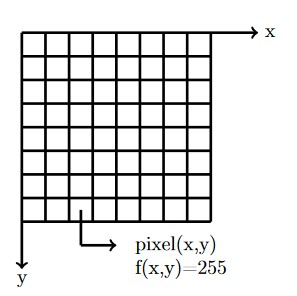
\includegraphics[height=5cm]{imagens/capitulo2/imagemCinza.jpg}}
    \subfloat[]{
        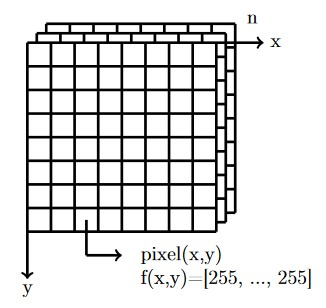
\includegraphics[height=5cm]{imagens/capitulo2/imagemColorida.jpg}}
    \caption{Exemplo de subfiguras usando o pacote \texttt{subfig}. Representação de uma imagem digital. (a) Imagem em escala de cinza. (b) Imagem colorida. Imagem extraída de \parencite{Barbosa2020}.}
    \label{fig:subfig}
\end{figure}

\begin{listing}[ht]
	\begin{minted}[linenos=true, baselinestretch=1, autogobble, bgcolor=Cornsilk1]{tex}
		\begin{figure}[ht]
		  \centering
		  \subfloat[]{
		    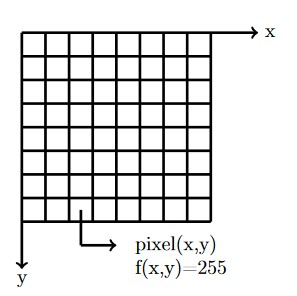
\includegraphics[height=5cm]{imagens/capitulo2/imagemCinza.jpg}}
		  \subfloat[]{
		    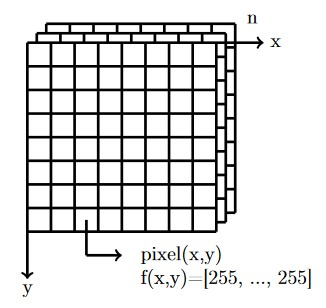
\includegraphics[height=5cm]{imagens/capitulo2/imagemColorida.jpg}}
		  \caption{Exemplo de subfiguras usando o pacote \texttt{subfig}. 
		  Representação de uma imagem digital. (a) Imagem em escala de cinza. 
		  (b) Imagem colorida. Imagem extraída de \parencite{Barbosa2020}.}
		  \label{fig:subfig}
		\end{figure}
	\end{minted}
	\caption{Código usado para organizar subfiguras usando o pacote \texttt{subfig}.}
	\label{cod:subfig}
\end{listing}

Como alternativa, você pode usar o ambiente \texttt{tabular}\index{tabular} para organizar as subfiguras e seus rótulos. A Figura \ref{fig:subfigtabular} foi criada usando este outro modo de organizar subfiguras. O Código \ref{cod:subfigtabular} mostra os comandos usados para gerá-la.

\begin{figure}[H]
	\begin{center}
		\begin{tabular}{cc}
			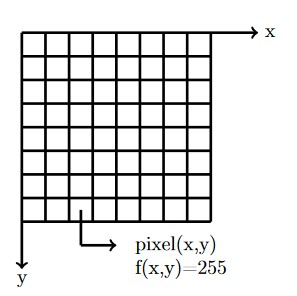
\includegraphics[height=5cm]{imagens/capitulo2/imagemCinza.jpg} & 
			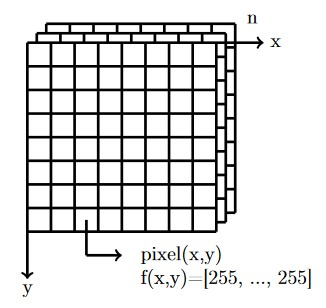
\includegraphics[height=5cm]{imagens/capitulo2/imagemColorida.jpg} \\
			(a) & (b) 
		\end{tabular}
	\end{center}
	\caption{Exemplo de subfiguras\index{subfiguras} usando o ambiente \texttt{tabular}. Representação de uma imagem digital. (a) Imagem em escala de cinza. (b) Imagem colorida. Imagem extraída de \parencite{Barbosa2020}.}
	\label{fig:subfigtabular}
\end{figure}

\begin{listing}[ht]
	\begin{minted}[linenos=true, baselinestretch=1, autogobble, bgcolor=Cornsilk1]{tex}
		\begin{figure}[ht]
		  \begin{center}
		    \begin{tabular}{cc}
		      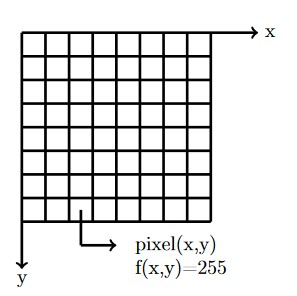
\includegraphics[height=5cm]{imagens/capitulo2/imagemCinza.jpg} & 
		      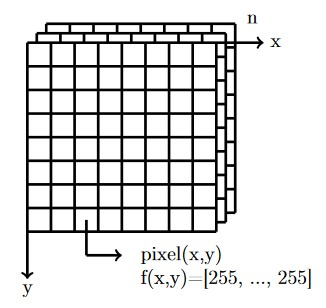
\includegraphics[height=5cm]{imagens/capitulo2/imagemColorida.jpg} 
		      \\
		      (a) & (b) 
		    \end{tabular}
		  \end{center}
		  \caption{Exemplo de subfiguras usando o ambiente \texttt{tabular}. 
		  Representação de uma imagem digital. (a) Imagem em escala de cinza. 
		  (b) Imagem colorida. Imagem extraída de \parencite{Barbosa2020}.}
		  \label{fig:subfigtabular}
		\end{figure}
	\end{minted}
	\caption{Código usado para organizar subfiguras usando o ambiente \texttt{tabular}.}
	\label{cod:subfigtabular}
\end{listing}

Você pode comparar visualmente os resultados das duas opções descritas acima observando as \Cref{fig:subfig,fig:subfigtabular}. Lembre-se que no caso do pacote \texttt{subfig}\index{subfig}, você pode referenciar e listar as subfiguras separadamente. Para maiores detalhes sobre o pacote \texttt{subfig}, consulte seu manual, que está disponível em \url{http://mirrors.ctan.org/macros/latex/contrib/subfig/subfig.pdf} \parencite{subfig}.

\section{Tabelas}

Tabelas são um outro tipo de objeto \texttt{float}\index{float} presente no \LaTeX{}. Existem páginas, capítulos de livros e até livros completos dedicados a criação de tabelas  em \LaTeX{}. Geralmente, se utiliza um ambiente tabular dentro de um objeto \texttt{float} do tipo \texttt{table}\index{table}. Esse ambiente tabular é responsável por informar quantas colunas uma tabela terá, e por sua tabulação, organizando os dados usando delimitadores pré-definidos.

\begin{table}[H]
	\centering
	\resizebox{\textwidth}{!}{%
		\begin{tabular}{|l|l|l|l|l|l|}
			\hline
			Tecido & Distância e Tamanho & Acurácia & Especificidade  & Sensibilidade & Coeficiente de Dice \\ \hline
			\multirow{2}{*}{Granulação} & $9 \times 9$\_E & $0,9252 \pm 0,0796$ & \textbf{$0,8961 \pm 0,1520$} & $0,8478 \pm 0,1942$ & $0,8796 \pm 0,1699$ \\ \cline{2-6}
			& $11 \times 11$\_E\_CSR & \textbf{$0,9292 \pm 0,0755$} & $0,8828 \pm 0,1673$ & \textbf{$0,8983 \pm 0,0914$} & \textbf{$0,9224 \pm 0,0650$} \\ \hline
			\multirow{2}{*}{Necrótico} & $9 \times 9$\_E & \textbf{$0,9595 \pm 0,0518$} & $0,9739 \pm 0,0436$ & $0,8758 \pm 0,8800$ & $0,8215 \pm 0,3155$ \\ \cline{2-6}
			& $11 \times 11$\_E\_CSR & $0,9591 \pm 0,0514$ & \textbf{$0,9741 \pm 0,0379$} & \textbf{$0,8963 \pm 0,0638$} & \textbf{$0,9037 \pm 0,1195$} \\  \hline
			\multirow{2}{*}{Esfacelo} & $9 \times 9$\_E & \textbf{$0,9346 \pm 0,0840$} & \textbf{$1,0000 \pm 0,0000$} & $0,8018 \pm 0,1489$ & \textbf{$0,8825 \pm 0,0983$} \\ \cline{2-6}
			& $11 \times 11$\_E\_CSR & $0,9336 \pm 0,0854$ & \textbf{$1,0000 \pm 0,0000$} & \textbf{$0,8111 \pm 0,1378$} & $0,8707 \pm 0,1089$ \\  \hline
			\multirow{2}{*}{Todos} & $9 \times 9$\_E & $0,9482 \pm 0,0457$ & $0,9784 \pm 0,0309$ & $0,8932 \pm 0,0771$ & $0,9234 \pm 0,0673$ \\ \cline{2-6}
			& $11 \times 11$\_E\_CSR & \textbf{$0,9491 \pm 0,0423$} & \textbf{$0,9788 \pm 0,0298$} & \textbf{$0,8952 \pm 0,0717$} & \textbf{$0,9247 \pm 0,0625$} \\ \hline
		\end{tabular}%
	}
	\caption{Resultados de uma tarefa de agrupamento. Adaptada de \parencite{Marques2018}.}
	\label{tab:resultadosVitor}
\end{table}

A Tabela \ref{tab:resultadosVitor} (adaptada de \parencite{Marques2018}) mostra resultados de uma tarefa de classificação. Neste exemplo, usei o pacote \texttt{multirow}\index{multirow} \parencite{multirow}, que permite criar multilinhas\index{multilinhas} e multicolunas\index{multicolunas}, centralizando o texto dentro dessas células compostas. O Código \ref{cod:tabresultadosVitor} mostra os comandos usados para gerar a Tabela \ref{tab:resultadosVitor}.

\begin{listing}[H]
	\begin{minted}[linenos=true, baselinestretch=1, autogobble, bgcolor=Cornsilk1]{tex}
	\begin{table}[H]
	  \centering
	  \resizebox{\textwidth}{!}{%
	  \begin{tabular}{|l|l|l|l|l|l|}
	    \hline
	    Tecido & Distância e Tamanho & Acurácia & Especificidade  
	    & Sensibilidade & Coeficiente de Dice \\ \hline
	    \multirow{2}{*}{Granulação} & $9 \times 9$\_E & $0,9252 
	    \pm 0,0796$ & \textbf{$0,8961 \pm 0,1520$} & $0,8478 \pm 0,1942$ 
	    & $0,8796 \pm 0,1699$ \\ \cline{2-6}
	    & $11 \times 11$\_\_CSR & \textbf{$0,9292 \pm 0,0755$} & 
	    $0,8828 \pm 0,1673$ & \textbf{$0,8983 \pm 0,0914$} & 
	    \textbf{$0,9224 \pm 0,0650$} \\ \hline
	    \multirow{2}{*}{Necrótico} & $9 \times 9$\_E & 
	    \textbf{$0,9595 \pm 0,0518$} & $0,9739 \pm 0,0436$ &
	    $0,8758 \pm 0,8800$ & $0,8215 \pm 0,3155$ \\ \cline{2-6}
	    & $11 \times 11$\_E\_CSR & $0,9591 \pm 0,0514$ & 
	    \textbf{$0,9741 \pm 0,0379$} & \textbf{$0,8963 \pm
	    0,0638$} & \textbf{$0,9037 \pm 0,1195$} \\ \hline
	    \multirow{2}{*}{Esfacelo} & $9 \times 9$\_E & 
	    \textbf{$0,9346 \pm 0,0840$} & \textbf{$1,0000 \pm
	    0,0000$} & $0,8018 \pm 0,1489$ & \textbf{$0,8825 \pm
	    0,0983$} \\ \cline{2-6}
	    & $11 \times 11$\_E\_CSR & $0,9336 \pm 0,0854$ & 
	    \textbf{$1,0000 \pm 0,0000$} & \textbf{$0,8111 \pm
	    0,1378$} & $0,8707 \pm 0,1089$ \\ \hline
	    \multirow{2}{*}{Todos} & $9 \times 9$\_E & $0,9482 
	    \pm 0,0457$ & $0,9784 \pm 0,0309$ & $0,8932 \pm 
	    0,0771$ & $0,9234 \pm 0,0673$ \\ \cline{2-6}
	    & $11 \times 11$\_E\_CSR & \textbf{$0,9491 \pm 0,0423$} 
	    & \textbf{$0,9788 \pm 0,0298$} & \textbf{$0,8952 \pm 0,0717$} & 
	    \textbf{$0,9247 \pm 0,0625$} \\ \hline
	  \end{tabular}%
	  }
	  \caption{Melhores resultados do agrupamento, adaptada de 
	  \parencite{Marques2018}.}
	  \label{tab:resultadosVitor}
	\end{table}
	\end{minted}
	\caption{Código usado para gerar a Tabela \ref{tab:resultadosVitor}.}
	\label{cod:tabresultadosVitor}
\end{listing}

Além do estilo padrão de tabelas do \LaTeX{}, que é bem permissivo, pode-se utilizar o pacote \texttt{booktabs}\index{booktabs} \parencite{booktabs}, que é conhecido pelo estilo de suas tabelas, similar a tabelas presentes em livros. Entretanto, o \texttt{booktabs} tem algumas restrições que foram impostas por escolhas de diagramação feitas pelos seus autores, como a impossibilidade de se usar linhas verticais separando colunas de uma tabela, a adição de um espaço acima e abaixo de linhas horizontais, a existência de linhas de diferentes espessuras e a impossibilidade do uso de linhas de separação duplas. Assim como as tabelas do estilo padrão do \LaTeX{}, as tabelas do \texttt{booktabs} podem ter suas linhas ou colunas coloridas usando os pacotes \texttt{xcolor}\index{xcolor} ou \texttt{colortbl}\index{colortbl}. O manual do pacote \texttt{booktabs} pode ser acessado em \url{http://mirrors.ctan.org/macros/latex/contrib/booktabs/booktabs.pdf} \parencite{booktabs}. 

Caso você tenha problemas no início para gerar suas tabelas, você pode utilizar algumas das páginas na Internet que permitem a criação de tabelas em \LaTeX{} de modo interativo, como o Tables Generator\index{Tables Generator} (\url{https://www.tablesgenerator.com/}) e o \LaTeX{} Tables\index{\LaTeX{} Tables} (\url{https://www.latex-tables.com/}). Algumas delas ainda permitem que se importem dados de arquivos de vários tipos, como \texttt{.csv}\index{.csv}, \texttt{.xls}\index{.xls} e \texttt{.ods}\index{.ods}.

Se você desejar criar tabelas muito elaboradas, podendo inclusive conter ilustrações, então eu sugiro que considere criá-las usando Ti\textit{k}Z\index{Ti\textit{k}Z}, que será abordado no Capítulo \ref{cap:desenhos}. Vários exemplos de tabelas criadas usando Ti\textit{k}Z estão disponíveis na Internet. 

\section{Algoritmos}

O pacote \texttt{algorithm2e}\index{algorithm2e} define um ambiente para escrever algoritmos em \LaTeXe, que são definidos como objetos \textit{float}\index{float} como figuras e tabelas. A apresentação dos algoritmos é bastante configurável.  As opções mostradas no Código \ref{cod:algorithm2e-setup} indicam que os algoritmos serão numerados por capítulo (\texttt{algochapter}\index{algochapter}), terão suas linhas numeradas (\texttt{linesnumbered}\index{linesnumbered}), exceto por comentários e entrada/saída, imprime linhas verticais delimitando blocos (\texttt{lined}\index{lined}), usa as palavras chaves em Português (portuguese) e escolhe o estilo \texttt{ruled}\index{ruled} como padrão para mostrar os algoritmos.

\begin{listing}[ht]
	\begin{minted}[linenos=true, autogobble, bgcolor=Cornsilk1]{tex}
	  \usepackage[algochapter, linesnumbered, lined, portuguese, ruled]
	  {algorithm2e}
	\end{minted}
	\caption{Exemplo de código \LaTeX{} usado para configuração do \texttt{algorithm2e}.}
	\label{cod:algorithm2e-setup}
\end{listing}

\begin{algorithm}[ht]
  \setstretch{1.35}
  $y = x.right$ \\
  $x.right = y.left$ \\
  \If{$y.left \neq T.nil$}{
    $y.left.p = x$}
  $y.p = x.p$ \\
  \If{$x.p == T.nil$}{
    $T.root = y$
  }
  \ElseIf{$x == x.p.left$}{
    $x.p.left = y$}
  \Else{$x.p.right = y$}
  $y.left = x$ \\
  $x.p == y$
  \caption{LeftRotate($T,x$)}
  \label{alg:left-rotate}
\end{algorithm}

No Algoritmo \ref{alg:left-rotate} vemos o código usado para realizar a rotação à esquerda em torno de um nó em uma árvore rubro-negra. Note o efeito das opções mencionadas acima na formatação do algoritmo. No Código \ref{cod:left-rotate} vemos os comandos definidos no pacote \texttt{algorithm2e}\index{algorithm2e} que foram usados para gerar o Algoritmo \ref{alg:left-rotate}. O comando da Linha 2 foi usado para diminuir o espaçamento entre linhas, já que este documento está usando espaçamento duplo.

\begin{listing}
	\begin{minted}[linenos=true, autogobble, bgcolor=Cornsilk1]{tex}
	\begin{algorithm}[ht]
	  \setstretch{1.35}
	  $y = x.right$ \\
	  $x.right = y.left$ \\
	  \If{$y.left \neq T.nil$}{
	    $y.left.p = x$}
	  $y.p = x.p$ \\
	  \If{$x.p == T.nil$}{
	    $T.root = y$}
	  \ElseIf{$x == x.p.left$}{
	    $x.p.left = y$}
	  \Else{$x.p.right = y$}
	  $y.left = x$ \\
	  $x.p == y$
	  \caption{LeftRotate($T,x$)}
	  \label{alg:left-rotate}
	\end{algorithm}
	\end{minted}
	\caption{Exemplo de código definido por \texttt{algorithm2e} usado para gerar o Algoritmo \ref{alg:left-rotate}.}
	\label{cod:left-rotate}
\end{listing}

Existem várias opções de formatação e numeração dos algoritmos, deste modo, sugiro que você leia o manual, que está disponível em \url{http://mirrors.ctan.org/macros/latex/contrib/algorithm2e/doc/algorithm2e.pdf} \parencite{algorithm2e} e teste os estilos disponíveis para que escolha o que lhe agrada mais.

\section{Código}\label{sec:codigo}

O pacote \texttt{minted}\index{minted} define os ambientes \texttt{minted} e \texttt{listings}\index{listings} para receber blocos de código. O primeiro gera o código e coloca em um retângulo com cor de fundo (\textit{background}\index{background}) que pode ser redefinida, enquanto que o segundo coloca o código em uma caixa do tipo \textit{float}\footnote{Um objeto do tipo \textit{float}\index{float} é um objeto que se move no documento de acordo com a escolha do \textit{kernel}\index{kernel} do \LaTeX{} para gerar a melhor diagramação possível.}.

O usuário pode então usar o comando mostrado no Código \ref{cod:listoflistings} para gerar uma lista de códigos ou \textit{listings}\index{listings}. Esse comando deve ser chamado no \textit{frontmatter}\index{frontmatter} do documento, junto com as listas de figuras, tabelas e algoritmos.

\begin{listing}[ht]
	\begin{minted}[linenos=true, autogobble, bgcolor=Cornsilk1]{tex}
	\texttt{listoflistings}	
	\end{minted}
\caption{Comando usado para gerar uma lista de \textit{listings} ou códigos.}
\label{cod:listoflistings}
\end{listing}

O pacote \texttt{minted}\index{} provê suporte para mais de 300 linguagens de programação. Para obter uma lista de todas elas, digite o comando abaixo em um terminal:

\adjustbox{fbox, center}{\texttt{pygmentize -L lexers}}

\begin{bclogo}[
	couleur=bgblue,
	arrondi=0,
	logo=\faWarning,%\bcbombe,
	barre=none,
	noborder=true]{Cuidado!}
	É importante mencionar que o pacote \texttt{minted} usa \texttt{Pygments}\index{Pygment}, um pacote de realçamento de texto escrito em Python\index{Python}. Como esse é um comando externo, você tem que habilitar a execução de comandos externos em sua ferramenta de edição \LaTeX{} (caso esteja usando uma) e usar o flag \texttt{-}\texttt{-shell-escape} no comando do processador utilizado, no nosso caso, o \hologo{pdfLaTeX}\index{\hologo{pdfLaTeX}}.
\end{bclogo}

O exemplo do Código \ref{cod:primo} mostra um exemplo do uso dos ambientes \texttt{minted}\index{minted} e \texttt{listing}\index{listing} para mostrar um código em C\index{C} em um objeto \texttt{float}\index{float}.

\begin{listing}[ht]
\begin{minted}[linenos=true, autogobble, bgcolor=Cornsilk1]{c}
#include <stdio.h>
#include <math.h>
void main() {
  int cont=0, n, i;
  printf("Digite um número: ");
  scanf("%d", &n);
  for(i=2; i<= floor(sqrt(n)); i++){
    printf("i = %d\n", i);   
    if (n%i == 0) {
      cont++;
      break;
  }      
} 
if (cont) 
  printf("%d não é primo\n", n);
else
  printf("%d é primo\n", n);
}
\end{minted}
\caption{Exemplo de código inserido em um \textit{listing}\index{listing}.}
\label{cod:primo}
\end{listing}

Para mais detalhes, você pode consultar o manual do \texttt{minted}\index{minted} ou o guia básico do \texttt{minted} no \gls{overleaf}\index{Overleaf}, disponíveis em 
\url{http://mirrors.ctan.org/macros/latex/contrib/minted/minted.pdf} \parencite{minted} e
\url{https://www.overleaf.com/learn/latex/Code_Highlighting_with_minted}, respectivamente.




  % Capitulo 3: Trabalhos Relacionados
   %% Capítulo 3

\chapter{Trabalhos Relacionados}\label{cap:trabalhos-relacionados}

Este capítulo apresenta os principais trabalhos encontrados na literatura que possuem temas ou áreas de atuação relacionadas à proposta neste estudo. São destacados trabalhos que exploram o desenvolvimento de questões de programação baseada em templates e técnicas associadas, bem como, as palavras de busca utilizada para localizar esses trabalhos.

\section{Metodologia de Busca}

A busca pelos trabalhos relacionados foi realizada utilizando palavras-chaves definidas previamente, empregadas em bases acadêmicas reconhecidas, como IEEE Xplore, Scopus e ACM Digital Library. A expressão de busca utilizada foi: 

\begin{quote}
\texttt{TITLE-ABS-KEY ( ( \textcolor{blue}{automatic} \textcolor{gray}{OR} \textcolor{blue}{automated} ) \textcolor{gray}{AND} \textcolor{blue}{item} \textcolor{gray}{AND} \textcolor{blue}{generation} \textcolor{gray}{AND} ( \textcolor{blue}{programming} \textcolor{gray}{OR} \textcolor{blue}{exercises} ) ) \textcolor{gray}{PUBYEAR >} \textcolor{orange}{2019} \textcolor{gray}{AND} \textcolor{gray}{PUBYEAR <} \textcolor{orange}{2025}}
\end{quote}

O período considerado abrangeu de janeiro de 2018 a novembro de 2024.  O processo de busca foi estruturado para identificar pesquisas relevantes na área de geração automática de questões de programação. A busca inicial resultou em 164 artigos. Após análise preliminar baseada nos títulos e resumos, os trabalhos foram filtrados  os trabalhos com base nas questões de pesquisa, conforme os critérios de inclusão e exclusão definidos conforme apresentado a seguir. 

\subsection{Critérios de Inclusão}
\begin{itemize}
    \item Relevância direta ao tema proposto
    \item Publicação dentro do período de 2018 a 2024.
    \item Fontes confiáveis.
    \item Disponibilidade completa do texto
    \item Uso explicito de templates para geração de questões de programação.
\end{itemize}
\subsection{Critérios de Exclusão}
\begin{itemize}
    \item Trabalhos fora do escopo do uso de templates para questões de programação. 
    \item Publicações com metodologias pouco detalhadas. 
    \item O artigo não está escrito em inglês .
    \item Artigos sem acesso completo. 
\end{itemize}

\section{Processo de Seleção}
A busca resultou inicialmente em 164 artigos. Após uma análise preliminar dos títulos e resumos, foram selecionados 10 estudos considerados relevantes para leitura detalhada. Em seguida, uma triagem mais criteriosa foi realizada com base nos critérios de inclusão e exclusão definidos previamente, o que reduziu o número final para 5 estudos incluídos nesta dissertação. Embora o repositório digital da \gls{acm} \textit{Digital Library} tenha retornado títulos e resumos altamente pertinentes ao escopo deste trabalho, o acesso restrito a essa base de dados dificultou significativamente a incorporação de um número maior de estudos relevantes. A tabela a seguir apresenta de forma detalhada a distribuição dos artigos encontrados em cada base de dados consultada, bem como a quantidade de estudos selecionados após o processo de triagem.

\begin{table}[htbp]
    \centering
    \begin{tabular}{|c|c|c|}
        \hline
        Base & Quantidade & Trabalhos Selecionados \\ \hline
        ACM Digital Library & 81 & 2 \\ \hline
        IEEE Xplore & 54 & 1 \\ \hline
        Scopus & 29 & 2 \\ \hline
        Total & 164 & 5 \\ \hline
    \end{tabular}
    \caption{Trabalhos selecionados}
    \label{tab:table-trabalhos-selecionados}
\end{table}


\section{Trabalhos Selecionados}
Esta seção apresenta diferentes abordagens relacionadas à geração automática de questões de programação, com foco no uso de templates e nas limitações identificadas em termos de variação e personalização. A análise ressalta a falta de integração com tecnologias avançadas, como inteligência artificial generativa e modelos multicamadas, e explora o potencial dessas ferramentas para ampliar a diversidade das questões e oferecer feedback automatizado. Além disso, a comparação com avanços registrados em áreas como a medicina demonstra a viabilidade de adaptar essas metodologias ao contexto do ensino e avaliação em questões de programação. 

\subsection{Zavala e Mendoza 2023}

Os estudos de \parencite{zalava2018} e   \parencite{zalava2023}  apresentam contribuições complementares no campo da geração automática de questões de programação utilizando templates e dados abertos interligados (\gls{lod}). Em 2018, os autores empregaram templates com variáveis e fórmulas embutidas, resolvidas automaticamente por um programa de computador, o que permitiu a criação de grandes bancos de questões a partir de um único template. No entanto, essa metodologia apresentou limitações na diversidade, com pouca variação contextual e estrutural das questões geradas. Posteriormente, na pesquisa de \parencite{zalava2023}, a incorporação de \gls{lod} possibilitou preencher automaticamente os templates com dados provenientes de fontes externas confiáveis, permitindo a criação de questões voltadas à programação e abrangendo uma gama mais ampla de tópicos. Embora essa abordagem tenha acelerado o processo de automação e reduzido erros humanos na validação de respostas, ainda enfrenta limitações, pois os templates utilizados oferecem variações predominantemente unidimensionais, sem explorar formatos mais diversificados na apresentação das questões.

 \subsection{Teubl, Ramos Batista e Zampirolli 2021}
O trabalho de \parencite{teubl2021}  apresenta o \textbf{MakeTests}, uma ferramenta que utiliza templates altamente parametrizados para gerar e corrigir automaticamente provas com diferentes estilos de questões, incluindo múltipla escolha, verdadeiro ou falso, correspondência, numérica e dissertativa. A principal contribuição da ferramenta reside na flexibilidade para criação de questões individualizadas, permitindo a geração de variações a partir de um modelo básico, o que reduz significativamente o trabalho manual dos professores.  A ferramenta também utiliza automação para correção de provas, no entanto a correção é feita por testes automatizados com respostas pré-definidas, limitando assim a interpretação das respostas dos alunos. Apesar dessas vantagens, a ferramenta requer conhecimento intermediário em Python para a criação de novos templates, o que pode ser uma barreira para alguns usuários. Portanto, há uma necessidade identificada de desenvolver uma interface mais acessível que elimine a exigência de habilidades de programação, tornando a ferramenta mais inclusiva para educadores com diferentes níveis de expertise técnica. 

\subsection{\text{Lehtinen, Santos e Sorva 2021}}
\parencite {lehtinen2021} propuseram um modelo para gerar perguntas automáticas baseadas no código escrito por estudantes, conhecido como  \gls{qlcs}. O processo utiliza análise estática e dinâmica do código em conjunto com templates predefinidos para criar questões personalizadas e relevantes. Primeiramente, o código do estudante é analisado para identificar elementos padrões, como estruturas condicionais, loops, variáveis e saídas. Com base nesses elementos, o sistema seleciona templates adequados e preenche-os automaticamente com informações específicas do código analisado. Esta abordagem melhorar a compreensão dos alunos sobre seus próprios códigos. 

 \subsection{\text{Saatz 2024}}
Como proposto por \parencite {saatz2024} , a geração automática de questões pode ser usada para resolução de problemas em contextos de computação  por meio de um fluxo de trabalho estruturado em duas etapas. O autor apresenta uma abordagem baseada em modelos no primeiro estágio e no uso de \textit{templates}  no segundo para criar questões níveis de dificuldade controlada, evitando repetitividade e possíveis fraudes nas avaliações. Como principais contribuições, se destaca a separação entre conteúdo, modelo de domínio e parâmetros de apresentação, a flexibilização na criação de diferentes tipos de questão e a simplificação do processo de criação de grandes de questões. Entre os trabalhos futuros, existe a necessidade de integração com ferramentas de inteligência artificial para aprimorar personalização do feedback dos estudantes. 


\section{\text{Analise comparativa}}

Na análise comparativa apresentada na tabela \ref{tab:table-comparativa-trabalhos-selecionados}, embora todos os trabalhos selecionados utilizam templates para gerar questões, no entando, não adotam uma abordagem multicamadas nem fazem uso de IA generativa para criação de variações nas questões. Além disso, até o momento não foram encontrados estudos acessíveis que utilizem templates combinados com IA generativa para sugerir variações e gerar feedback automatizado especificamente no contexto de geração de questões de programação. 

\begin{table}[htbp]
    \centering
    \begin{tabular}{|l|c|c|c|}
        \hline
        Autor& Templates & Multicamadas & IA Generativa \\ \hline
        Zavala e Mendoza 2018& \faCheck & \faClose& \faClose\\ \hline 
        Zavala e Mendoza 2023 & \faCheck&  \faClose& \faClose\\ \hline
        Teubl, Ramos Batista e Zampirolli 2021 & \faCheck& \faClose& \faClose\\\hline
        Lehtinen, Santos e SorvaSaatz 2024 & \faCheck & \faClose&\faClose \\\hline
        Silva, A. de S. 2025 (este trabalho)& \faCheck & \faCheck&\faCheck \\\hline
    \end{tabular}
    \caption{Tabela comparativa dos trabalhos selecionados (Elaboração própria, 2025)}
    \label{tab:table-comparativa-trabalhos-selecionados}
\end{table}


Como mostra a Tabela \ref{tab:table-comparativa-trabalhos-selecionados}, os trabalhos anteriores utilizam modelos de template de camada única, exigindo maior intervenção manual para gerar variações de enunciado e revisar a qualidade das questões. A ausência de uma arquitetura multicamadas limita a flexibilidade estrutural, enquanto a falta de IA generativa inviabiliza a criação automática de novos contextos. A contribuição deste trabalho é aplicar os templates multicamadas e adicionar modelos de IA generativa para preencher este espaço identificado na literatura e também adicionar um fluxo de trabalho diferente na geração de questões de programação.
Na área da saúde, como a medicina, a aplicação de templates multicamadas e de IA generativa para a geração automática de questões e feedback automatizado já é uma prática amplamente utilizada. Estudos como \parencite{falcao2023} e \parencite{kiyak2024} indicam que a IA generativa pode produzir questões de alta qualidade, contribuindo tanto para a avaliação quanto para o aprimoramento contínuo do processo de criação de questões. Esses avanços sugerem que, com as adaptações necessárias, a geração automática de questões tem um grande potencial para ser implementada com sucesso na área de programação.
No entanto, essa oportunidade ainda depende de iniciativas de pesquisadores e desenvolvedores dispostos a adaptar e aplicar as metodologias validadas na medicina ao contexto específico do desenvolvimento de questões de programação.

No próximo capítulo, serão apresentados os fundamentos teóricos que embasam este trabalho.  Serão explorados os conceitos essenciais do modelo cognitivo aplicado à elaboração de questões e o papel dos templates multicamadas na automação do processo, estabelecendo a base teórica para futuras discussões. 





   % Capitulo 4: Fundamentação Teórica
 % Capítulo 4
\chapter{Fundamentação Teórica}\label{cap:fundamentacao-teorica}

Este capítulo está organizado para introduzir os conceitos-chave e explicar detalhadamente cada seção. Serão apresentados os fundamentos teóricos que sustentam o desenvolvimento e a aplicação de dois modelos fundamentais para a implementação da proposta: o modelo cognitivo e o modelo de template multicamadas para geração automática de questões. Cada subseção abordará os conceitos essenciais relacionados a esses modelos, detalhando suas características, funcionamento e contribuições para o objetivo final do estudo.

\section{Modelo Cognitivo}
A construção de questões em larga escala, por meio de processos automatizados, tem-se tornado uma prática cada vez mais relevante na área de avaliações educacionais. Nesse contexto, a elaboração de um modelo cognitivo sólido constitui um passo fundamental para embasar a Geração Automática de Questões (\gls{aig}). De modo geral, modelos cognitivos podem ser definidos como descrições explícitas de como os estudantes processam informações e resolvem tarefas específicas, envolvendo as habilidades e os raciocínios que se espera que demonstrem em uma dada questão. O processo de construção desse modelo, conforme discutido por \parencite{gierl2021}, esta técnica consiste em identificar, organizar e documentar de forma sistematizada os conceitos, parâmetros e restrições que caracterizam tanto a criação de uma questão quanto a forma como os estudantes são esperados a resolvê-la.

A relevância do modelo cognitivo torna-se ainda mais evidente quando se busca a replicabilidade e a qualidade das questões geradas em larga escala. Esse detalhamento fornece a base para a elaboração dos templates, os quais orientam a criação de questões capazes de manter o mesmo nível de complexidade, exigência cognitiva e alinhamento ao conteúdo que se deseja avaliar. Dessa forma, o modelo cognitivo funciona como um roteiro que descreve tanto os conteúdos quanto a lógica da questão a ser gerada.

O modelo cognitivo é a base fundamental para a criação dos templates, pois organiza e descreve todos os elementos necessários para sua construção. Os templates, por sua vez, atuam como estruturas que convertem essas informações de forma efetiva, resultando em questões de avaliação individual claras e alinhadas aos objetivos de ensino.


\section{Estrutura do Modelo Cognitivo}

O modelo cognitivo funciona como um guia para organizar os elementos necessários para a construção dos templates. Estes templates servem como estruturas que traduzem as diretrizes estabelecidas no modelo cognitivo em questões, claras, consistentes e alinhadas aos objetivos educacionais \parencite{keehner2017, gierl2017}. Para garantir a qualidade e replicabilidade, o modelo cognitivo deve ser estruturado de maneira a detalhar os seguintes aspectos fundamentais : 

\section{Definição de Problemas e Cenários}

A primeira etapa do processo de construção do modelo cognitivo consiste em definir claramente o objetivo da avaliação, identificando o problema central que servirá de base. Em uma disciplina de algoritmos que aborda estruturas de repetição, podemos optar por explorar aspectos como o tipo de laço ou os componentes fundamentais de uma estrutura controlada por um contador. Dessa forma, podemos assegurar que as habilidades específicas a serem avaliadas estejam claramente refletidas na questão. E, posteriormente, elaborar possíveis cenários relacionados ao problema principal. Nas avaliações sobre estruturas de repetição em programação, podemos incluir cenários que envolvam a identificação do tipo de laço utilizado em um trecho de código, a utilização de contadores para controlar iterações ou a aplicação de estruturas de repetição em situações práticas de desenvolvimento de algoritmos. Cada cenário amplia a diversidade das questões, mantendo a coerência com o objetivo da avaliação.

\section{Fontes de Informação}

As fontes de informação constituem o conjunto de conteúdos e matérias que podem abranger dados quantitativos, textos, fórmulas, diagramas, trechos de código, figuras ou qualquer outro elemento que possibilite aos estudantes acionarem os conhecimentos e habilidades que se deseja avaliar. Cada fonte de informação deve ser descrita de forma detalhada, de modo a estabelecer claramente a relação entre o conteúdo apresentado e as características a serem avaliadas.


\section{Características (\textit{Features})}



As características (\textit{features}) são atributos fundamentais que compõem os as dimensões ou variáveis variável do modelo cognitivo. Elas definem os aspectos que podem ser ajustados na criação dos templates. Na prática,cada característica é composta por elementos, valores e restrições:


\subsubsection{Elementos}
Representam os componentes básicos de cada característica. Podem ser, por exemplo, uma variável numérica, um trecho de código ou um termo técnico relevante para a questão. Os elementos ajudam a identificar claramente as informações que serão utilizadas na formulação das questões.


\subsubsection{Valores}
São as diferentes opções que cada elemento pode assumir. Podem ser números, palavras-chave ou formatos específicos, como tipos de laços de repetição em programação (por exemplo, \texttt{for}, \texttt{while}, \texttt{do-while}). Os valores determinam as variações possíveis de um elemento, permitindo a geração de questões diversificadas.

\subsubsection{Restrições (\textit{Constraints})}
As restrições estabelecem as regras que evitam combinações de elementos que gerem itens inválidos ou sem sentido. Por exemplo, é possível restringir a geração de problemas que incluam números negativos quando o objetivo for mensurar apenas operações básicas com inteiros positivos. Essas regras impedem a geração aleatória e asseguram a criação de itens alinhados às metas instrucionais e ao nível de dificuldade desejado.

As restrições estabelecem regras ou condições que limitam como os elementos e seus valores podem ser combinados de tal forma que evite a construção de questões sem lógica, inválidas ou sem sentido. É esperado que com as restrições, as combinações resultantes durante a geração sejam coerentes e significativas. 

% ----------------------------------------------------------
% Trechos da Seção 5 (Avaliação do Modelo)
% ----------------------------------------------------------

\paragraph{}A etapa de avaliação do modelo cognitivo é fundamental para garantir que o processo de geração de itens mantenha consistência teórica e prática. Inicialmente, um especialista diferente daquele que construiu o modelo pode revisá-lo, analisando a coerência das fontes de informação, a adequação das características definidas e a pertinência das restrições estabelecidas. Esse especialista verifica se as instruções, os valores e a lógica de montagem refletem adequadamente o problema que se pretende medir, apontando eventuais inconsistências ou ambiguidades no modelo.

\paragraph{}Em seguida, recomenda-se a avaliação externa ou independente, na qual outro grupo de especialistas, que não participou do desenvolvimento prévio, fornece um parecer sobre a clareza, a completude e a precisão do modelo. O uso de escalas ou rubricas de julgamento pode sistematizar e documentar as impressões dos avaliadores, permitindo refinar ainda mais o modelo. Essa avaliação adicional contribui para validar o processo de geração de itens e para assegurar sua qualidade em aplicações futuras.




O modelo cognitivo é a base fundamental para a criação dos templates, pois organiza e descreve todos os elementos necessários para sua construção. Os templates, por sua vez, atuam como estruturas que convertem essas informações de forma efetiva, resultando em questões de avaliação individual claras e alinhadas aos objetivos de ensino.
O modelo cognitivo é o elemento base para processo da geração automática de questões, pois determina as diretrizes de como o conhecimento e as habilidades devem ser organizados para criar questões em larga escala \cite{gierl2016, gierl2017, gierlbulutzhang2018, keehner2017}. É a partir desse modelo que se definem, de maneira estruturada, aspectos como:

\begin{itemize} \item Conteúdos a serem avaliados (conceitos, regras e relações); \item Habilidades e processos de pensamento esperados dos estudantes (como identificar, analisar, resolver problemas); \item Restrições e parâmetros de combinação (limites numéricos, coerência semântica, condições mínimas para a aplicação de um conceito). \end{itemize}



\section{Relação do Modelo Cognitiva e Construção de Templates }

Por outro lado, os \textit{templates} são estruturas que convertem o modelo cognitivo em modelos práticos de questões \cite{gierl2024}. Cada \textit{template} especifica como as informações do modelo serão incorporadas ao enunciado e às alternativas (corretas e incorretas). Assim, a relação entre o modelo cognitivo e os \textit{templates} pode ser resumida nos seguintes pontos:

\begin{enumerate} \item \textbf{Definição de elementos básicos de uma questão:} O modelo cognitivo descreve quais componentes (por exemplo, dados quantitativos, termos-chave, situações-problema) precisam estar presentes para que o item seja relevante e alinhado aos objetivos pedagógicos. O \textit{template} organiza esses componentes em uma estrutura pronta para gerar diferentes versões de questão \cite{lane2016}.
\item \textbf{Combinação e manipulação de parâmetros:} Enquanto o modelo cognitivo define as regras de como os conteúdos e as habilidades podem ser combinados (por exemplo, valores ou conceitos que podem variar para alterar a dificuldade de um item), o \textit{template} coloca essas regras em prática. Em outras palavras, integra os diversos elementos para criar itens com diferentes níveis de complexidade, mantendo a coerência com a proposta original \cite{embretson2017}.

\item \textbf{Padronização e escalabilidade:} A adoção de um modelo cognitivo bem elaborado facilita a padronização do processo de elaboração de itens em grande escala. Como os \textit{templates} seguem o mesmo conjunto de regras e estruturas, as questões criadas tendem a manter consistência em termos de conteúdo, formato e nível de exigência cognitiva \cite{gierl2016, gierl2017}.

\item \textbf{Validação e ajustes contínuos:} Se um \textit{template} gerar um item que se revele muito fácil ou muito difícil, é possível identificar rapidamente se o problema está no modelo cognitivo ou no próprio \textit{template}, permitindo o ajuste da regra que originou a inconsistência. Dessa forma, a correção ocorre em nível conceitual (no modelo) ou técnico (na estrutura do \textit{template}), preservando a qualidade dos itens e mantendo-os alinhados aos propósitos da avaliação \cite{gierlbulutzhang2018}.
\end{enumerate}
Em síntese, o modelo cognitivo oferece a base teórica e estrutural, descrevendo de forma clara o que e por que está sendo avaliado, enquanto o \textit{template} representa a forma de aplicação prática dessas informações na formulação das questões \cite{gierl2024}. Essa integração torna a Geração Automática de Questões mais sólida, pois cada item criado segue a mesma lógica e mantém um padrão de qualidade, contribuindo para avaliações mais consistentes e confiáveis.

\section{Modelo de Template}

\subsubsection{Template 1-Layer}
\subsubsection{Template N-Layers}



  % Capitulo 4: Quarto capítulo (arquivo capitulos/capitulo4.tex)
  %

% Capítulo 4
\chapter{Equações, Provas e Especificações}\label{cap:equa}

O intuito deste capítulo é o de introduzir os pacotes matemáticos que foram sugeridos por diversos professores, de acordo com suas necessidades, e mostrar exemplos simples de como usá-los. Ele não deve ser visto como texto introdutório, mediano ou avançado sobre como se deve usar os ambientes matemáticos disponíveis em \LaTeX{}. Existem vários excelentes livros e manuais físicos e digitais, pagos e gratuitos, que lidam com este extenso tópico, de modo que não usarei espaço neste capítulo para tal.

Como sugestões de referências sobre o uso de comandos e pacotes \LaTeX{} para a escrita de fórmulas matemáticas, elenco as seguintes:
\begin{enumerate}
	\item Short Math Guide for \LaTeX{} - Disponível em  \url{http://mirrors.ctan.org/info/short-math-guide/short-math-guide.pdf}
	\item \LaTeX{} Cookbook \parencite{Kottwitz2015} - Livro disponível em papel e eletronicamente.
	\item Overleaf - O \gls{overleaf}\index{Overleaf} separa pequenos textos introdutórios e com exemplos para diferentes tópicos relacionados à definição de equações. Um bom lugar para iniciar a leitura é \url{https://www.overleaf.com/learn/latex/mathematical_expressions}.
\end{enumerate}

\section{Equações}

Um dos principais objetivos de Knuth quando projetou o \TeX{} era o de permitir a construção de fórmulas matemáticas de modo simples, mas que tivessem qualidade profissional quando impressas. Então, ele definiu sintaxes para vários símbolos matemáticos e criou comandos para a representação de equações. 
Para que \TeX{} ou \LaTeX{} gere os símbolos matemáticos, eles precisam saber que o texto é matemático. Os textos matemáticos pode ser do tipo texto (ou \textit{inline}), isto é, os símbolos são colocados na linha de texto, ou equação, onde os símbolos são colocados na linha própria deles.

No caso dos textos matemáticos \textit{inline}, nós sinalizamos um texto matemático usando os delimitares \textbackslash ( e \textbackslash ), no caso do \LaTeX e \$ e \$, no caso do \TeX{} e \LaTeX{}. Deve-se ter cuidado para não colocar equações ou símbolos muito altos que acabem gerando em espaçamento muito grande entre linhas, o que pode gerar uma diagramação não agradável visualmente. Um exemplo de equação simples que pode caber em uma linha é \( E = m c^2 \), que foi gerada com o código
\texttt{\textbackslash ( E = mc\^{}2 \textbackslash )}.

Os textos matemáticos no formato equação podem ser numerados ou não. No caso das equações não numeradas, você pode usar os delimitadores \textbackslash [ e \textbackslash ] no caso do \LaTeX{} e \$\$ e \$\$, no caso do \TeX{} e \LaTeX{}. Caso esteja usando \texttt{amsmath}\index{amsmath} \parencite{amsmath} ou \texttt{mathtools}\index{mathtools} \parencite{mathtools}, você pode usar a versão ``*'' do ambiente \texttt{equation}, que suprime a numeração e contagem dos objetos. O mesmo vale para os outros ambientes definidos em \texttt{mathtools}, como \texttt{align}\index{align}, \texttt{flalign}\index{flalign}, \texttt{gather}\index{gather} e \texttt{multilined}\index{multilined}. 

Para usar a numeração das equações, você deve colocar os códigos das suas equações dentro de um ambiente (\textit{environment}\index{environment}) \texttt{equation}\index{equation}, que foi usado para gerar a Equação \ref{eq:raytracing}, que define a equação da interação da luz no ray-tracing recursivo, como pode ser visto no Código \ref{cod:raytracing}. Nesse caso, por causa do tamanho da equação, eu utilizei o ambiente \textit{multlined}\index{multlined} do \texttt{mathtools}\index{mathtools} (também incluído neste modelo) para quebrar a equação em duas linhas. Caso deseje alinhar os termos da equação, você pode usar o ambiente \texttt{aligned}\index{aligned}, também definido no \texttt{mathtools}\index{mathtools}. Neste exemplo, eu escolhi usar a representação das setas que indicam vetores do pacote \texttt{esvector}\index{esvector}, que permite que se selecione um dentre oito possíveis estilos de setas. Eu escolhi usar as setas do \texttt{esvector} somente nos vetores $\vv{N}$ e $\vv{V}$, para que você pudesse comparar com as aparências dos vetores $\overrightarrow{L}$ e $\overrightarrow{R}$, que foram criados usando as setas do \texttt{mathtools}. Caso necessite usar muitos símbolos matemáticos, sugiro que você veja os símbolos definidos pelo pacote \texttt{amsfonts}\index{amsfonts} (\url{http://mirrors.ctan.org/fonts/amsfonts/doc/amsfonts.pdf}) nos sub-pacotes \texttt{amssymb}\index{amssymb} (\url{http://mirrors.ctan.org/fonts/amsfonts/doc/amssymb.pdf}), \texttt{euscript}\index{euscript} (\url{http://mirrors.ctan.org/fonts/amsfonts/doc/euscript.pdf}) e \texttt{eufrak}\index{eufrak} (\url{http://mirrors.ctan.org/fonts/amsfonts/doc/eufrak.pdf}).
 
 
\begin{equation}
	\begin{multlined}
	  I_{\lambda} = \underbrace{ I_{a \lambda} K_a O_{d \lambda} }_{ambiente}   
	  + \sum f_{att} I_{p \lambda} \left[ \underbrace{ k_d O_{d \lambda} \left( \vv{N} \cdot \overrightarrow{L} \right)}_{difusa} + \underbrace{ k_s O_{s \lambda} \left( \overrightarrow{R} \cdot \vv{V}  \right)^n }_{especular} \right] \\ 
	  + \underbrace{k_s \left[ \underbrace{ \left( 1 - k_t \right) O_{s \lambda} }_{refletida} + \underbrace{ k_t O_{t \lambda} I_{t \lambda} }_{refratada} \right] }_{recursivo}
	\end{multlined}
    \label{eq:raytracing}
\end{equation}

\begin{listing}[ht]
	\begin{minted}[linenos=true, autogobble, bgcolor=Cornsilk1]{tex}
	\begin{equation}
	  \begin{multlined}
	    I_{\lambda} = \underbrace{ I_{a \lambda} K_a O_{d \lambda} 
	    }_{ambiente} + \sum f_{att} I_{p \lambda} \left[ 
	    \underbrace{ k_d O_{d \lambda} \left( \vv{N} \cdot 
	    \overrightarrow{L} \right)}_{difusa} + \underbrace{ k_s 
	    O_{s \lambda} \left( \overrightarrow{R} \cdot \vv{V}  
	    \right)^n }_{especular} \right] \\ 
	    + \underbrace{k_s \left[ \underbrace{ \left( 1 - k_t \right) 
	    O_{s \lambda} }_{refletida} + \underbrace{ k_t O_{t \lambda} 
	    I_{t \lambda} }_{refratada} \right] }_{recursivo}
	  \end{multlined}
	  \label{eq:raytracing}
	\end{equation}
	\end{minted}
	\caption{Código \LaTeX{} usado para gerar a Equação \ref{eq:raytracing}.}
	\label{cod:raytracing}
\end{listing}

Um pacote que pode auxiliá-lo eventualmente é o \texttt{siunitx}\index{siunitx}, que provê um conjunto de ferramentas para a diagramação de quantidades de um modo consistente. Por exemplo, a unidade $\si{kg.m/s^2}$ pode ser gerada usando um dos comandos mostrados no Código \ref{cod:sunitx}. No primeiro modo, o literal, o \texttt{siunitx} converte os símbolos ``.'' e ``\~{}'' nos espaços correspondentes e posiciona corretamente os subscritos e sobrescritos, enquanto que o modo ``textual'' usa o significado das unidades ao invés da aparência ditada pelo modo literal. O manual do pacote \texttt{siunitx} pode ser acessado em \url{http://mirrors.ctan.org/macros/latex/contrib/siunitx/siunitx.pdf} \parencite{siunitx}.

\begin{listing}[ht]
	\begin{minted}[linenos=true, autogobble, bgcolor=Cornsilk1]{tex}
	  \si{kg.m/s^2}
	  \si{\kilo\gram\meter\per\square\second}	
	\end{minted}
	\caption{Código \LaTeX{} usado para gerar a unidade $\si{\kilo\gram\meter\per\square\second}$.}
	\label{cod:sunitx}
\end{listing}

O pacote \texttt{amsmath}\index{amsmath} provê uma grande gama de melhorias para a organização e impressão de expressões matemáticas. Por exemplo, ele define novos ambientes para a diagramação de matrizes, amplia o leque de opções para espaçamento em equações, melhora a representação pictorial de letras com acentos, define setas extensíveis, dentre outros. Para mais detalhes, consulte o manual em \url{http://mirrors.ctan.org/macros/latex/required/amsmath/amsldoc.pdf} \parencite{amsmath}.

O pacote \texttt{mathtools}\index{mathtools} provê uma série de ferramentas projetadas para melhorar a aparência de documentos que contenham muitos símbolos matemáticos. Ele carrega o pacote \texttt{amsmath}, passando parâmetros para esse outro pacote quando necessário, além de definir vários novos símbolos, novos ambientes para equações e permitir que se numere somente equações referenciadas de forma automática. Ele ainda corrige alguns erros presentes no pacote \texttt{amsmath}\index{amsmath}. Como ele carrega o pacote \texttt{amsmath} quando é carregado, você pode omitir o carga do pacote \texttt{amsmath} quando usa o \texttt{mathtools}.

O exemplo abaixo mostra como podemos usar \texttt{mathtools}\index{mathtools} para ajustar o subscrito de um somatório, removendo espaçamento extra que faz a equação parecer desconectada. A Equação \ref{eq:sum} mostra a saída original enquanto que a Equação \ref{eq:sum_mathclap} mostra a versão usando o comando \texttt{\textbackslash mathclap}\index{mathclap}, cujo uso pode ser visto no Código \ref{cod:mathclap}.

\begin{equation}
	 T = \sum_{1\le i\le j\le n} X_{ij}
	 \label{eq:sum}
\end{equation}

\begin{equation}
	T = \sum_{\mathclap{1\le i\le j\le n}} X_{ij}
	\label{eq:sum_mathclap}
\end{equation}

\begin{listing}[ht]
	\begin{minted}[linenos=true, autogobble, bgcolor=Cornsilk1]{tex}
	\begin{equation}
	  T = \sum_{\mathclap{1\le i\le j\le n}} X_{ij}
	  \label{eq:sum_mathclap}
	\end{equation}
	\end{minted} 
	\caption{Exemplo do uso do comando \textbackslash \texttt{mathclap}.}
	\label{cod:mathclap}
\end{listing}

O pacote \texttt{mathtools}\index{mathtools} ainda define novos ambientes de matrizes, similares aos definidos no \texttt{amsmath}\index{amsmath}, mas que permitem que o alinhamento dos elementos seja configurado e não sempre centralizado, como no \texttt{amsmath}. 

O pacote ainda provê vários comandos para que se façam ajustes finos em elementos de equações. Para conhecê-los, acesse o manual do \texttt{mathtools}\index{mathtools} em 
\url{http://mirrors.ctan.org/macros/latex/contrib/mathtools/mathtools.pdf} \parencite{mathtools}.

Existem vários editores de equações online, que permitem que você teste a escrita de suas equações e veja os resultados. Você ainda terá que digitar os comandos das equações como se estivesse em um documento \LaTeX{}. Alguns exemplos dessas ferramentas são o \TeX{} Equation Editor\index{\TeX{} Equation Editor} \url{http://atomurl.net/math/}, o CodeCogs\index{CodeCogs} (\url{https://www.codecogs.com/latex/eqneditor.php}), o HostMath\index{HostMath} (\url{https://www.hostmath.com/}) e o Latex4technics\index{Latex4technics} (\url{https://www.latex4technics.com/}).

Algumas ferramentas de edição de código matemático para \LaTeX{} foram desenvolvidas para serem executadas localmente, como o EqualX\index{EqualX} \url{https://equalx.sourceforge.io/} e o AxMath\index{AxMath} \url{https://www.axsoft.co/}, sendo que esta última é uma solução paga, com o custo de US\$ 12.00 no momento da escrita deste parágrafo.

\begin{figure}[ht]
	\begin{center}
		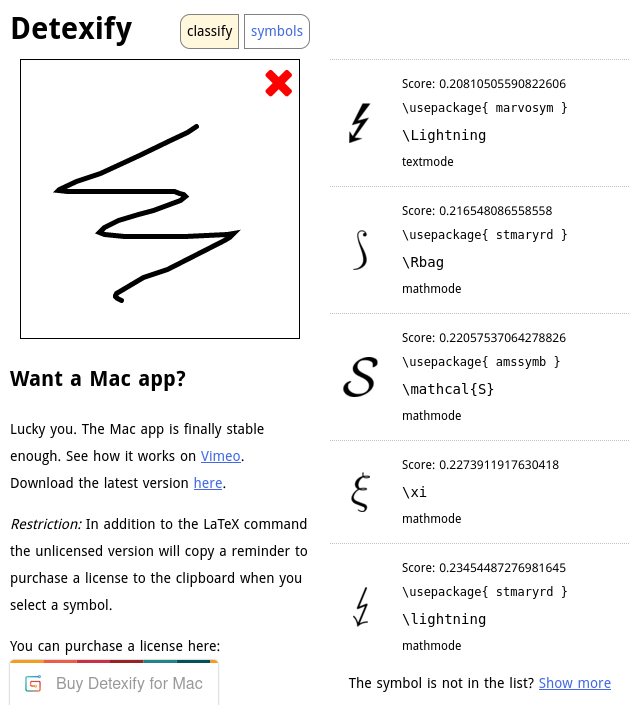
\includegraphics[scale=0.5]{./imagens/capitulo4/detexify.png}
		
	\end{center}
	\caption{Exemplo de uso da ferramenta \textit{online} detexify (\url{https://detexify.kirelabs.org/classify.html}).}
	\label{fig:detexify}
\end{figure}

Além dessas ferramentas, você pode utilizar o LyX\index{LyX} (\url{https://www.lyx.org/}), um editor de textos \gls{wysiwym}, que está disponível para Linux, Windows e Mac OS, e que é construído em cima do \LaTeX{}, e que permite se construir facilmente não só equações usando uma interface gráfica, mas também ambientes tabulares complexos para inserção em tabelas.

Finalmente, gostaria de indicar uma ferramenta simples, mas que pode ser bastante útil quando você quer incluir um símbolo matemático no seu documento mas esqueceu do nome dele em \LaTeX{}. Se este é o seu caso, visite a página do detexify\index{detexify}
\url{https://detexify.kirelabs.org/classify.html} e desenhe uma aproximação do símbolo no janela indicada e um software de classificação vai indicar quais símbolos são mais parecidos com o seu desenho, qual é o nome do comando que representa o símbolo e o pacote ao qual ele pertence. Um exemplo do uso desta ferramenta pode ser visto na Figura \ref{fig:detexify}.

\section{Provas} 

Existem vários pacotes que auxiliam na criação de provas de diversos estilos. Neste modelo, incorporamos alguns desses pacotes, os quais descrevemos brevemente a seguir. O primeiro pacote a ser apresentado é o \texttt{bussproofs}, um pacote que permite que se construa árvores de provas no estilo de cálculo de sequentes e outros sistemas de provas. Esse pacote define o comando \texttt{\textbackslash{}fCenter}, que define um ponto central para uso no alinhamento horizontal. Abaixo vemos um exemplo do uso do pacote \texttt{bussproofs}\index{bussproofs}, seguido dos comandos usados para gerá-lo, no Código \ref{cod:bussproofs}, inclusive do comando \texttt{\textbackslash{}fCenter}. 

\def\fCenter{\mbox{\Large$\rightarrow$}}
\begin{prooftree}
	\Axiom$\Gamma, A, B\ \fCenter\ B$
	\UnaryInf$\Gamma, A\ \fCenter\ (B \to C)$
	\UnaryInf$\Gamma\ \fCenter\ (A \to (B \to C))$
\end{prooftree}

\begin{listing}[ht]
	\begin{minted}[linenos=true, autogobble, bgcolor=Cornsilk1]{tex}
		\def\fCenter{\mbox{\Large$\rightarrow$}}
		\begin{prooftree}
		  \Axiom$\Gamma, A, B\ \fCenter\ B$
		  \UnaryInf$\Gamma, A\ \fCenter\ (B \to C)$
		  \UnaryInf$\Gamma\ \fCenter\ (A \to (B \to C))$
		\end{prooftree}
	\end{minted} 
	\caption{Exemplo do uso do pacote \texttt{bussproofs}. Exemplo extraído de \parencite{bussproofs}.}
	\label{cod:bussproofs}
\end{listing}

O endereço \url{http://mirrors.ctan.org/macros/latex/contrib/bussproofs/testbp2.pdf} permite que se acesse um pequeno documento contendo exemplos do uso do pacote enquanto que o manual pode ser acessado em \url{http://mirrors.ctan.org/macros/latex/contrib/bussproofs/BussGuide2.pdf} \parencite{bussproofs}.

Já o pacote \texttt{lplfitch}\index{lplfitch} provê macros para a diagramação de provas por dedução natural no estilo ``Fitch'', com as sub-provas indentadas e linhas de escopo. A tentativa do uso desse pacote com pacotes das classes de documentos do \gls{koma} gerou erros por conflito devido ao uso de pacotes descontinuados pelo \TeX{} mas que ainda funcionam com classes mais antigas como a \texttt{book}\index{book} e \texttt{article}\index{article}. Para que este pacote funcione com as classes do modelo \gls{koma}\index{\hologo{KOMAScript}}, as duas linhas do Código \ref{cod:lplfitch-setup} devem ser definidas no preâmbulo do seu documento.

\begin{listing}[ht]
	\begin{minted}[linenos=true, autogobble, bgcolor=Cornsilk1]{tex}
	\DeclareOldFontCommand{\sf}{\normalfont\sffamily}{\mathsf}
	\DeclareOldFontCommand{\bf}{\normalfont\bfseries}{\mathbf}
	\end{minted} 
	\caption{Comandos necessários para o uso do pacote \texttt{lplfitch} \parencite{lplfitch} com as classes do modelo \gls{koma}\index{\hologo{KOMAScript}}.}
	\label{cod:lplfitch-setup}
\end{listing}

O exemplo abaixo mostra uma prova no estilo produzido pelo pacote \texttt{lplfitch}\index{lplfitch}, que pode ser incluído em um objeto \texttt{float}\index{float} \texttt{figure}\index{figure} ou apresentado sozinho. Devido a como o pacote \texttt{lplfitch} foi implementado, sugiro que você coloque comandos escolhendo o espaçamento simples antes e duplo após a prova, como pode ser visto no Código \ref{cod:lplfitch}. Caso isso não seja feito, os espaços entre as linhas das provas ficam muito grandes e o efeito não é muito bom.

\singlespacing
\fitchprf{}{
	\subproof{\pline[1.]{\uni{x}{(Cube(x)\lif Small(x))}}}{
		\subproof{\pline[2.]{\exi{x}{Cube(x)}}}{
			\boxedsubproof[3.]{a}{Cube(a)}{
				\pline[4.]{Cube(a)\lif Small(a)}[\lalle{1}]\\
				\pline[5.]{Small(a)}[\life{4}{3}]\\
				\pline[6.]{\exi{x}{Small(x)}}[\lexii{5}]
			}
			\pline[7.]{\exi{x}{Small(x)}}[\lexie{2}{3--6}]
		}
		\pline[8.]{\exi{x}{Cube(x)}\lif \exi{x}{Small(x)}}[\lifi{2--7}]
	}
	\pline[9.]{\brokenform{(\uni{x}{(Cube(x)\lif Small(x))}\lif}{
			\formula{(\exi{x}{Cube(x)} \lif \exi{x}{Small(x)})}}}[\lifi{1--8}]
}
\doublespacing

\begin{listing}[ht]
	\begin{minted}[linenos=true, autogobble, bgcolor=Cornsilk1]{tex}
	\singlespacing
	\fitchprf{}{
	  \subproof{\pline[1.]{\uni{x}{(Cube(x)\lif Small(x))}}}{
	    \subproof{\pline[2.]{\exi{x}{Cube(x)}}}{
	      \boxedsubproof[3.]{a}{Cube(a)}{
	        \pline[4.]{Cube(a)\lif Small(a)}[\lalle{1}]\\
	        \pline[5.]{Small(a)}[\life{4}{3}]\\
	        \pline[6.]{\exi{x}{Small(x)}}[\lexii{5}]
	      }
	      \pline[7.]{\exi{x}{Small(x)}}[\lexie{2}{3--6}]
	    }
	    \pline[8.]{\exi{x}{Cube(x)}\lif \exi{x}{Small(x)}}[\lifi{2--7}]
	  }
	  \pline[9.]{\brokenform{(\uni{x}{(Cube(x)\lif Small(x))}\lif}{
	      \formula{(\exi{x}{Cube(x)} \lif \exi{x}{Small(x)})}}}[\lifi{1--8}]
	}
	\doublespacing
	\end{minted} 
	\caption{Comandos necessários para o uso do pacote \texttt{lplfitch} \parencite{lplfitch} com as classes do modelo \gls{koma}.}
	\label{cod:lplfitch}
\end{listing}

\bigskip

O manual do pacote \texttt{lplfitch}\index{lplfitch} pode ser acessado em \url{http://mirrors.ctan.org/macros/latex/contrib/lplfitch/lplfitch.pdf} \parencite{lplfitch}.

Diferente dos pacotes vistos acima, o pacote \texttt{natded}\index{natded} implementa ferramentas para criar provas de dedução natural nos estilos de Jaśkowski e Kalish-Montague. O exemplo exemplo abaixo mostra uma prova escrita no estilo de Kalish-Montague (exemplo extraído de \parencite{natded}) e os comandos usados para gerá-la podem ser vistos no Código \ref{cod:natded}. A Linha 2 do Código \ref{cod:natded} foi incluída para diminuir o espaçamento entre linhas pois o pacote \texttt{natded} gera caixas com linhas não contíguas quando o espaçamento é duplo, como neste modelo. 

\begin{equation*}
\setstretch{1.3}
\KMproof{
	\cbblk{
		\proofline{((( P \rightarrow Q ) \land (\neg R \rightarrow \neg Q ) ) \rightarrow ( P \rightarrow R ) ) }{2 -- 13
Conditionalization}
	}{
		\proofline{(( P \rightarrow Q ) \land (\neg R \rightarrow \neg Q ) )}{Supposition}
		\cbblk{
			\proofline{( P \rightarrow R ) }{4 -- 13 Conditionalization}
		}{
			\proofline{ P }{Supposition}
			\proofline{(( P \rightarrow Q ) \land (\neg R  \rightarrow \neg Q ) ) }{2 Repeat}
			\proofline{( P \rightarrow Q )}{5 Simplification}
			\proofline{ Q }{4, 6 Modus Ponens}
			\proofline{(\neg R \rightarrow \neg Q )}{5 Simplification}
			\cbblk{
				\proofline{ R }{10 -- 13 Reductio ad Absurdum}
			}{
				\proofline{\neg R }{ Supposition}
				\proofline{(\neg R \rightarrow \neg Q ) }{8 Repeat }
				\proofline{\neg Q }{10 , 11 Modus Ponens}
				\proofline{ Q }{7 Repeat}
			}
		}
	}
}
\end{equation*}



O pacote \texttt{natded}\index{natded} disponibiliza o manual em \url{http://mirrors.ctan.org/macros/latex/contrib/natded/natded.pdf} \parencite{natded}, de onde foi extraído o exemplo acima, e a documentação extra em \url{http://mirrors.ctan.org/macros/latex/contrib/natded/extended_doc.pdf} \parencite{natded-extra}.

\section{Especificações}

Especificações formais usam notações matemáticas para modelar precisamente as propriedades que um sistema computacional deve possuir. Existem várias linguagens criadas para descrever essa propriedades. Neste modelo, incorporamos os pacotes das linguagens CSP\index{CSP}, Z\index{Z} e Circus\index{Circus}. Caso você não necessite usá-las, comente os comandos \texttt{\textbackslash usepackage} correspondentes.
 
 \begin{listing}[ht]
 	\begin{minted}[linenos=true, autogobble, bgcolor=Cornsilk1]{tex}
\begin{equation*}
  \setstretch{1.3}
  \KMproof{
    \cbblk{
      \proofline{((( P \rightarrow Q ) \land (\neg R \rightarrow 
        \neg Q ) ) \rightarrow ( P \rightarrow R ) ) }{2 -- 13
        Conditionalization}
     }{
      \proofline{(( P \rightarrow Q ) \land (\neg R \rightarrow 
        \neg Q ) ) }{Supposition}
      \cbblk{
        \proofline{( P \rightarrow R ) }{4 -- 13 Conditionalization}
      }{
        \proofline{ P }{ Supposition }
        \proofline{(( P \rightarrow Q ) \land (\neg R  \rightarrow 
          \neg Q ) ) }{2 Repeat}
        \proofline{( P \rightarrow Q ) }{5 Simplification}
        \proofline{ Q }{4, 6 Modus Ponens }
        \proofline{(\neg R \rightarrow \neg Q ) }{5 Simplification}
        \cbblk{
          \proofline{ R }{10 -- 13 Reductio ad Absurdum }
        }{
          \proofline{\neg R }{ Supposition}
          \proofline{(\neg R \rightarrow \neg Q ) }{8 Repeat}
          \proofline{\neg Q }{10 , 11 Modus Ponens}
          \proofline{ Q }{7 Repeat}
        }
      }
    }
 }
\end{equation*}
 	\end{minted} 
 	\caption{Exemplo do uso do pacote \texttt{natded}.}
 	\label{cod:natded}
 \end{listing}

O pacote \texttt{zed-csp}\index{zed-csp} é um pacote que foi desenvolvido baseado no pacote original \texttt{zed}\index{zed}, que implementa a diagramação no formato da linguagem Z\index{Z} e incluiu as definições para CSP\index{CSP}. O exemplo abaixo mostra o uso do ambiente de definição genérica (\texttt{gendef}\index{gendef}), criado pelo pacote \texttt{zed-csp}\index{zed-csp}, e os comandos usados para gerar este exemplo, extraído de \parencite{zed}\index{zed}, podem ser vistos no Código \ref{cod:zed-csp}.
 
\begin{gendef}[X,Y]
	first: X \cross Y \fun X
\where
		\forall x: X; y: Y @ \\
\t1     first(x,y) = x
\end{gendef}

\begin{listing}[ht]
	\begin{minted}[linenos=true, autogobble, bgcolor=Cornsilk1]{tex}
		\begin{gendef}[X,Y]
		  first: X \cross Y \fun X
		\where
		  \forall x: X; y: Y @ \\
		\t1     first(x,y) = x
		\end{gendef}
	\end{minted} 
	\caption{Exemplo do uso do pacote \texttt{zed-csp}.}
	\label{cod:zed-csp}
\end{listing}

O pacote \texttt{zed-csp}\index{zed-csp} possui dois manuais, um para a linguagem CSP\index{CSP} \url{http://mirrors.ctan.org/macros/latex/contrib/zed-csp/csp2e.pdf} \parencite{csp} e o outro para Z\index{Z} \url{http://mirrors.ctan.org/macros/latex/contrib/zed-csp/zed2e.pdf} \parencite{zed}. 

Existe um outro pacote para a criação de especificações em Z\index{Z}, o \texttt{objectz}\index{objectz}. Entretanto eu não carreguei ambos os pacotes para verificar se \texttt{objectz} e \texttt{zed-csp} são compatíveis, já que definem ambientes com os mesmos nomes. Caso precise usar o \texttt{objectz}, eu sugiro que apenas substitua o pacote \texttt{zed-csp}\index{zed-csp}. O manual do \texttt{objectz} pode ser acessado em \url{http://mirrors.ctan.org/macros/latex/contrib/objectz/ozguide.pdf} \parencite{objectz}.








% Capitulo 5: Proposta Conceitual
\chapter{Proposta Conceitual}

...

  % Capitulo 5: Quinto capítulo (arquivo capitulos/capitulo5.tex)
  %% Capítulo 5
\chapter{Desenhos e Animações}\label{cap:desenhos}

Neste capítulo, descreverei brevemente os pacotes de auxílio a desenhos que são recomendados para uso com este modelo. Como parte ainda experimental, adicionei um pacote que permite incluir animações em documentos \gls{pdf}\index{pdf}, embora elas só possam ser visualizadas em leitores de \gls{pdf} que processam JavaScript\index{JavaScript}.

A gama de pacotes que facilitam a criação de desenhos em \LaTeX{} é imensa, e vai desde grandes ambientes de programação a pequenos pacotes auxiliares. Aqui, vamos ver brevemente alguns desses ambientes e pacotes auxiliares. Esse capítulo dá uma maior ênfase ao ambiente de geração de ilustrações definidos pela dupla de linguagens \gls{pgf}/\gls{tikz}\index{Ti\textit{k}Z}, sendo que \gls{pgf}\index{PGF} é uma linguagem de alto nível e Ti\textit{k}Z é um conjunto de macros de alto nível que usa PGF.

\section{Qtree} \label{qtree}

O pacote \texttt{qtree}\index{qtree} oferece suporte para o desenho de árvores, e é comumente utilizado em aplicações de linguística. Ele emprega uma sintaxe simples usando colchetes e calcula automaticamente os tamanhos dos ramos. A Figura \ref{fig:qtree} foi gerada usando o comando mostrado do Código \ref{cod:cod-qtree}.

\begin{figure}
\Tree [.S [.DP [.D O ] [.NP jogador ] ] [.VP \qroof{chutou a bola}.VP [.AdvP bisonhamente ] ] ]
\caption{Exemplo simples de árvore gerada usando o pacote qtree.}
\label{fig:qtree}
\end{figure}

\begin{listing}[ht]
	\begin{minted}[ linenos=true, autogobble, bgcolor=Cornsilk1 ]{tex}
	\Tree [.S [.DP [.D O ] [.NP jogador ] ] [.VP \qroof{chutou a bola}.VP 
	[.AdvP bisonhamente ] ] ]
	\end{minted}
	\caption{Exemplo de código \LaTeX{} usado para gerar a árvore da Figura \ref{fig:qtree}.}
	\label{cod:cod-qtree}
\end{listing}

Para maiores detalhes e outros exemplos do uso de \texttt{qtree}, você pode utilizar \url{http://mirrors.ctan.org/macros/latex/contrib/qtree/qtreenotes.pdf} \parencite{qtree}.

\section{Ti\textit{k}Z e Pacotes Auxiliares} \label{sec:tikz}

O pacote \texttt{tikz}\index{Ti\textit{k}Z} (geralmente escrito em documentos como Ti\textit{k}Z) é provavelmente a ferramenta mais potente para a criação de gráficos em \LaTeX{}. Ele implementa várias funções de desenho e serve como base para vários outros pacotes associados que criam facilidades para que se produzam desenhos com certas especialidades. Till Tantau projetou as linguagens \gls{pgf} e \gls{tikz}, sendo que o nome Ti\textit{k}Z representa o acrônimo recursivo ``Ti\textit{k}Z \textit{ist kein Zeichenprogramm}'', que em Português significa ``Ti\textit{k}Z não é um programa de desenho''.

Uma busca recente feita por mim no \gls{ctan} com o termo ``tikz'' gerou uma lista com 205 pacotes. Como o intuito aqui é o de introduzir o uso de Ti\textit{k}Z\index{Ti\textit{k}Z} e não cobrir de um grande número de pacotes, veremos aqui apenas alguns exemplos.

Outra opção bastante utilizada para desenhar em \LaTeX{} é o pacote PSTricks\index{PSTricks}, que também é muito bom. Entretanto, devido a sua melhor compatibilidade com o \hologo{pdfLaTeX}\index{\hologo{pdfLaTeX}}, escolhi o Ti\textit{k}Z como pacote básico de desenho para este modelo.

Como no caso dos outros pacotes, o Ti\textit{k}Z\index{Ti\textit{k}Z} pode ser incluído simplesmente usando o comando: 

\adjustbox{fbox, center}{\texttt{\textbackslash usepackage\{tikz\}}}

Abaixo, no Código \ref{cod:cod-tikz-pre} nós vemos alguns comandos que podem ser necessários executar antes de se usar o Ti\textit{k}Z\index{Ti\textit{k}Z}, dependendo do tipo de desenho que deseje produzir. O comando da Linha 1 carrega o pacote \texttt{bclogo} e informa que o pacote gráfico a ser utilizado é o Ti\textit{k}Z, pois o \texttt{bclogo} também funciona com o PSTricks\index{PSTricks}. As Linhas 2 e 3 carregam dois pacotes que se baseiam no Ti\textit{k}Z para realizar desenhos de grafos de dependência e redes, respectivamente, enquanto que as Linhas 4 e 5 carregam dois pacotes que foram implementados em formato de bibliotecas Ti\textit{k}Z. Finalmente, as Linhas 6, 7 e 8 definem e configuram \textit{layers} (camadas), que são necessárias para alguns casos.

\begin{listing}[ht]
	\begin{minted}[ linenos=true, autogobble, bgcolor=Cornsilk1 ]{tex}
		\usepackage[tikz]{bclogo}
		\usepackage{tikz-dependency}
		\usepackage{tikz-network}
		\usetikzlibrary{switching-architectures}
		\usetikzlibrary{mindmap}
		\pgfdeclarelayer{background}
		\pgfdeclarelayer{foreground}
		\pgfsetlayers{background,main,foreground}
	\end{minted}
	\caption{Exemplo de código \LaTeX{} usado para configuração do Ti\textit{k}Z.}
	\label{cod:cod-tikz-pre}
\end{listing}

O pacote define o ambiente \texttt{tikzfigure}, que delimita o código de seu desenho. Geralmente colocamos o ambiente \texttt{tikzfigure} dentro de um ambiente \texttt{figure} para criar um objeto \texttt{float}\index{float}, como vimos no Capítulo \ref{cap:float}.

O desenho de linhas com e sem setas é extremamente simples, assim como o de outras primitivas gráficas, e as propriedades associadas a esses elementos. Abaixo, na Figura \ref{fig:tikz-ex1}, vemos um exemplo simples de desenho feito usando várias características de primitivas, e que foi gerado pelo Código \ref{cod:cod-tikz-ex1}. Na Linha 1 do código, um ambiente \texttt{tikzpicture} foi criado e teve a escala 2 associada a ele, ou seja, o gráfico terá o dobro do tamanho definido internamente. A Linha 2 desenha as linhas do sistema de coordenadas e a opção \texttt{<->} diz ao Ti\textit{k}Z\index{Ti\textit{k}Z} que setas devem ser desenhadas no início e final das linhas. As opções mostradas nas Linhas de 3 a 6 estabelecem as propriedades das primitivas desenhadas, como cor, espessura e padrão. Note como é simples desenhar uma linha, apenas definindo as coordenadas\footnote{As coordenadas no Ti\textit{k}Z são expressas em centímetros.} dos pontos entre parenteses e alternando eles com os caracteres \texttt{-}\texttt{-}.

\begin{figure}
	\begin{center}
		\begin{tikzpicture}[scale=2]
		  \draw [<->] (0,2) -- (0,0) -- (4,0);
		  \draw [blue, thick] (0,1.5) -- (3,0);
		  \draw [red, ultra thick] (0,0) -- (2,2);
		  \draw [dashed, help lines] (1,0) -- (1,1) -- (0,1);
		  \draw [green, thick] (1.45,1.065) circle [radius=0.25];
		\end{tikzpicture}
	\end{center}
\caption{Exemplo simples de gráfico elaborado usando Ti\textit{k}Z.}
\label{fig:tikz-ex1}
\end{figure}

\begin{listing}[ht]
	\begin{minted}[ linenos=true, autogobble, bgcolor=Cornsilk1 ]{tex}
		\begin{tikzpicture}[scale=2]
		  \draw [<->] (0,2) -- (0,0) -- (4,0);
		  \draw [blue, thick] (0,1.5) -- (3,0);
		  \draw [red, ultra thick] (0,0) -- (2,2);
		  \draw [dashed, help lines] (1,0) -- (1,1) -- (0,1);
		  \draw [green, thick] (1.45,1.065) circle [radius=0.25];
		\end{tikzpicture}
	\end{minted}
	\caption{Código \LaTeX{} usado para gerar exemplo de gráfico da Figura \ref{fig:tikz-ex1}.}
	\label{cod:cod-tikz-ex1}
\end{listing}

O Ti\textit{k}Z\index{Ti\textit{k}Z} também nos permite desenhar facilmente gráficos de equações como pode ser visto na Figura \ref{fig:tikz-ex2}, que foi gerada com o Código \ref{cod:cod-tikz-ex2}. Observe como é simples se gerar gráficos com funções conhecidas. Caso você queira desenhar gráficos de funções geradas por sequências de pontos, é só carregar as coordenadas dos pontos no formato Ti\textit{k}Z e ligá-los por retas. Note, entretanto, que nesse caso, uma ampliação do pdf iria salientar a falta de suavidade do gráfico, dependendo da amostragem utilizada na geração dos pontos.

\begin{figure}
	\begin{center}
		\begin{tikzpicture}[yscale=1.5]
			\draw [help lines, ->] (0,0) -- (6.5,0);
			\draw [help lines, ->] (0,-1.1) -- (0,1.1);
			\draw [green,domain=0:2*pi] plot (\x, {(sin(\x r)* ln(\x+1))/2});
			\draw [red,domain=0:pi] plot (\x, {sin(\x r)});
			\draw [blue, domain=pi:2*pi] plot (\x, {cos(\x r)*exp(\x/exp(2*pi))});
		\end{tikzpicture}
	\end{center}
	\caption{Exemplo de gráfico gerado com Ti\textit{k}Z.}
	\label{fig:tikz-ex2}
\end{figure}

\begin{listing}[ht]
	\begin{minted}[ linenos=true, autogobble, bgcolor=Cornsilk1 ]{tex}
	\begin{tikzpicture}[yscale=1.5]
	  \draw [help lines, ->] (0,0) -- (6.5,0);
	  \draw [help lines, ->] (0,-1.1) -- (0,1.1);
	  \draw [green,domain=0:2*pi] plot(\x,{(sin(\x r)*ln(\x+1))/2});
	  \draw [red,domain=0:pi] plot(\x,{sin(\x r)});
	  \draw [blue,domain=pi:2*pi] plot(\x,{cos(\x r)*exp(\x/exp(2*pi))});
	\end{tikzpicture}
	\end{minted}
	\caption{Código \LaTeX{} usado para gerar exemplo de gráfico da Figura \ref{fig:tikz-ex2}.}
	\label{cod:cod-tikz-ex2}
\end{listing}

Os manuais do Ti\textit{k}Z\index{Ti\textit{k}Z} podem ser acessados em \url{http://cremeronline.com/LaTeX/minimaltikz.pdf} \parencite{tikzintro} (manual introdutório) e \url{http://mirrors.ctan.org/graphics/pgf/base/doc/pgfmanual.pdf} \parencite{tikz} (manual oficial). Eu recomendo que tenha o manual oficial do Ti\textit{k}Z, caso precise gerar desenhos com frequência para os seus documentos. Ele é extremamente detalhado e contém muitos exemplos. Além disso, sugiro a página \url{https://texample.net/tikz/examples/}, que armazena muitos exemplos de desenhos gerados com vários pacotes, e que podem servir de base para algum desenho que precise gerar.

\begin{itemize}
	\item SA-Ti\textit{k}Z - O pacote \texttt{sa-tikz}\index{sa-tikz} define a biblioteca Sa-Ti\textit{k}Z que auxilia no desenho de arquiteturas de \textit{switching}\index{switching} (comutação) e define os modelos Clos, Benes e Banyan e algumas variações destes modelos. O pacote permite que se configure aspectos da rede como as dimensões do módulo, a distância entre módulos e a fonte usada. Por exemplo, a Figura \ref{fig:redeBanyan} mostra uma rede de \textit{switching} Banyan-Omega. Para maiores detalhes, consulte o manual, que está disponível em \url{http://mirrors.ctan.org/graphics/pgf/contrib/sa-tikz/doc/sa-tikz-doc.pdf} \parencite{sa-tikz}.

\begin{figure}[htb]
	\begin{center}
        \begin{tikzpicture}
    		% Omega Network on the left
    		\node[banyan omega] {};
    		\begin{scope}[xshift=7.25cm]
	    	% Flip network on the right
	    		\node[banyan flip]{};
    		\end{scope}
		\end{tikzpicture}
	\end{center}
	\caption{Exemplo de duas redes de \textit{switching} Banyan-Omega geradas usando a biblioteca \texttt{switching-architectures} do pacote \texttt{sa-tikz}. Exemplo extraído de \parencite{sa-tikz}.}
	\label{fig:redeBanyan}
\end{figure}

\item Bclogo - O pacote \texttt{bclogo}\index{bclogo} permite que se criem caixas coloridas com a inclusão de logotipos, o que é interessante para chamar a atenção para alguns trechos do documento. Esse pacote depende do pacote \texttt{mdframed}\index{mdframed}. Assim, mensagens importantes, como a mostrada abaixo, podem ter a devida atenção dos leitores.

\begin{bclogo}[
	couleur=bgblue,
	arrondi=0,
	logo=\faBeer,%\bcbombe,
	barre=none,
	noborder=true]{Você Sabia?}
	Você sabia que o consumo moderado de cerveja aumenta a densidade dos ossos em humanos? Um outro estudo mostrou que bebedores moderados têm um menor risco de doenças cardiovasculares do que os abstêmios!
\end{bclogo}

O manual do pacote \texttt{bclogo} (em Francês) pode ser acessado em 
 \url{http://mirrors.ctan.org/graphics/bclogo/doc/bclogo-doc.pdf} \parencite{bclogo}.

\item Ti\textit{k}Z-Dependency\index{Ti\textit{k}Z-Dependency} - O pacote \texttt{tikz-dependency} é um pacote que facilita a criação de grafos de dependência, comumente utilizados em algumas áreas de pesquisa, como grafos e processamento de linguagem natural. 

Ele permite que facilmente se definam estilos para os nós, arestas e rótulos, facilitando enormemente a produção desses grafos. A Figura \ref{fig:grafdep} mostra um exemplo simples feito usando \texttt{tikz-dependency}. Seu manual pode ser acessado em \url{http://mirrors.ctan.org/graphics/pgf/contrib/tikz-dependency/tikz-dependency-doc.pdf} \parencite{tikz-dependency}.

\begin{figure}[htb]
	\begin{center}
	\begin{dependency}[theme=copper]
		\begin{deptext}[column sep=0.2cm]
			My \&[.5cm] dog \& also \&[.7cm] likes \&[.4cm] eating \& sausage \\
		\end{deptext}
		\depedge{2}{1}{poss}
		\depedge{4}{2}{nsubj}
		\depedge{4}{3}{advmod}
		\depedge{4}{5}{xcomp}
		\depedge{5}{6}{dobj}
		\deproot{4}{root}
	\end{dependency}
	\end{center}
	\caption{Exemplo de grafo de dependência criado usando \texttt{tikz-dependency}. Exemplo extraído de \parencite{tikz-dependency}.}
	\label{fig:grafdep}
\end{figure}

\begin{listing}[ht]
	\begin{minted}[ linenos=true, autogobble, bgcolor=Cornsilk1 ]{tex}
	\begin{dependency}[theme=copper]
	  \begin{deptext}[column sep=0.2cm]
	    My \&[.5cm] dog \& also \&[.7cm] likes \&[.4cm] eating 
	    \& sausage \\
	  \end{deptext}
	  \depedge{2}{1}{poss}
	  \depedge{4}{2}{nsubj}
	  \depedge{4}{3}{advmod}
	  \depedge{4}{5}{xcomp}
	  \depedge{5}{6}{dobj}
	  \deproot{4}{root}
	\end{dependency}
	\end{minted}
	\caption{Código \LaTeX{} usado para gerar exemplo de gráfico da Figura \ref{fig:grafdep} usando a biblioteca definida pelo pacote \texttt{tikz-dependency}.}
	\label{cod:cod-grafdep}
\end{listing}

\item Ti\textit{k}Z-Network\index{Ti\textit{k}Z-Network} - Existem várias ferramentas que facilitam o desenho de redes ou grafos, como Xfig\index{Xfig} ou Inkscape\index{Inkscape}. Você pode utilizar uma dessas ferramentas e salvar o conteúdo desejado, de preferência em um formato vetorial, para posteriormente adicioná-las ao seu documento. 

Uma abordagem diferente permite que você desenhe sua rede ou grafo diretamente no documento \LaTeX{}, o que possibilita a realização de ajustes de estilos e tamanhos de fontes, adição de equações, e outras tarefas, sem que se precise retornar a um software externo. O pacote \texttt{tikz-network} permite que se crie e manipule desenhos de redes ou gráficos de maneira simples, gerando gráficos escaláveis que mantêm a qualidade quando o arquivo \gls{pdf}\index{PDF} é ampliado.

A Figura \ref{fig:grafnet} mostra um exemplo simples de rede que foi gerada carregando-se dois arquivos de configuração, um contendo os nós e o outro, as arestas.

\begin{figure}[htb]
	\begin{center}
	\begin{tikzpicture}[scale=1.5]
		\Vertices{./capitulos/vertices.csv}
		\Edges[lw=2.5]{./capitulos/edges.csv}
	\end{tikzpicture}
	\end{center}
	\caption{Exemplo de grafo criado usando \texttt{tikz-network}. Exemplo extraído de \parencite{tikz-network}.}
	\label{fig:grafnet}
\end{figure}

Esse pacote permite que se crie redes mais complexas, como a rede em multinível mostrada na Figura \ref{fig:grafnmn}, que foi gerada usando os comandos vistos no Código \ref{cod:cod-tikz-nmn}. O manual desse pacote pode ser acessado em 
\url{http://mirrors.ctan.org/graphics/pgf/contrib/tikz-network/tikz-network.pdf} \parencite{tikz-network}.

\begin{figure}[htb]
	\begin{center}
	\begin{tikzpicture}[multilayer=3d, scale=1.5]
	  \begin{Layer}[layer=1]
	    \Plane[x=-.5,y=-.5,width=2.5,height=3,grid=5mm]
	  \end{Layer}	 
	  \begin{Layer}[layer=2]
	    \Plane[x=-.5,y=-.5,width=2.5,height=3,grid=5mm]
	    \end{Layer}	
	  \Vertices{capitulos/ml-vertices.csv}
	  \Edges{capitulos/ml-edges.csv}
	\end{tikzpicture}
	\end{center}
\caption{Exemplo de grafo em multinível criado usando \texttt{tikz-network}\index{tikz-network}. Exemplo adaptado de \parencite{tikz-network}\index{tikz-network}.}
\label{fig:grafnmn}
\end{figure}

\begin{listing}[ht]
	\begin{minted}[ linenos=true, autogobble, bgcolor=Cornsilk1 ]{tex}
	\begin{tikzpicture}[multilayer=3d, scale=1.5]
	  \begin{Layer}[layer=1]
	    \Plane[x=-.5,y=-.5,width=2.5,height=3,grid=5mm]
	  \end{Layer}	 
	  \begin{Layer}[layer=2]
	    \Plane[x=-.5,y=-.5,width=2.5,height=3,grid=5mm]
	  \end{Layer}	
	  \Vertices{capitulos/ml-vertices.csv}
	  \Edges{capitulos/ml-edges.csv}
	\end{tikzpicture}
	\end{minted}
	\caption{Código \LaTeX{} usado para gerar exemplo de gráfico da Figura \ref{fig:grafnmn} usando a biblioteca definida pelo pacote \texttt{tikz-network}\index{tikz-network}.}
	\label{cod:cod-tikz-nmn}
\end{listing}

\item PGFPlots - O pacote \texttt{pgfplots}\index{PGFPlots} permite criar facilmente gráficos de alta qualidade em escalas lineares e logarítmicas em 2D e 3D usando uma interface amigável. A Figura \ref{fig:pgfplots} mostra um gráfico gerado usando esse pacote, com a sequência de comandos mostradas no código \ref{cod:pgfplots}.

% Preamble: \pgfplotsset{width=7cm,compat=1.17}
\begin{figure}[H]
	\begin{center}
		\begin{tikzpicture}[scale=1.5]
			\begin{axis}
				\addplot3 [ surf, domain=0:360,	samples=40,	] {sin(x)*sin(y)};
			\end{axis}
		\end{tikzpicture}
	\end{center}
	\caption{Exemplo de gráfico 3D impresso usando \texttt{pgfplots}\index{PGFPlots}.}
	\label{fig:pgfplots}
\end{figure}

\begin{listing}[ht]
	\begin{minted}[ linenos=true, autogobble, bgcolor=Cornsilk1 ]{tex}
		\begin{tikzpicture}[scale=1.5]
		  \begin{axis}
		    \addplot3 [ surf, domain=0:360, samples=40, ] {sin(x)*sin(y)};
		  \end{axis}
		\end{tikzpicture}
	\end{minted}
	\caption{Código \LaTeX{} usado para gerar exemplo de gráfico da Figura \ref{fig:pgfplots} usando o pacote \texttt{pgfplots}\index{PGFPlots}.}
	\label{cod:pgfplots}
\end{listing}

Algumas rotinas chamadas por este pacote, principalmente as 3D, podem ser demoradas, acarretando em aumento razoável do tempo de compilação do seu documento. Deste modo, analise se esta é a melhor opção ou se você deveria gerar os gráficos 3D fora do \LaTeX{} e importá-los.

O manual desse pacote pode acessado em \url{http://mirrors.ctan.org/graphics/pgf/contrib/pgfplots/doc/pgfplots.pdf} \parencite{pgfplots}, e muitos exemplos podem ser encontrados na Internet.

\item Como mais um exemplo de tipo específico de desenho, apresento uma figura gerada com o auxílio da bilbioteca \texttt{mindmaps}\index{mindmaps}. Essa biblioteca pode ser usada juntamente com o Ti\textit{k}Z para criar mapas mentais, que são diagramas usados para organizar informações visualmente. A Figura \ref{fig:mapamental} mostra um exemplo que elenca os capítulos desse documento, detalhando as subseções de alguns capítulos.

Certos cuidados devem ser tomados ao criar esses mapas mentais. Muitos ramos ou textos longos criam problemas na diagramação, que devem ser corrigidos alterando a escala e os ângulos entre os ramos. Mais detalhes podem ser acessados no tutorial para iniciantes em Ti\textit{k}Z do \gls{overleaf}\index{Overleaf}, que pode ser acessado em \url{https://www.overleaf.com/learn/latex/LaTeX_Graphics_using_TikZ:_A_Tutorial_for_Beginners_(Part_5)\%E2\%80\%94Creating_Mind_Maps}.

\begin{figure}[htb]
	\begin{center}
	\begin{tikzpicture}[mindmap, scale=0.9, grow cyclic, every node/.style=concept, concept color=orange!40, 
	level 1/.append style={level distance=5cm,sibling angle=45},
	level 2/.append style={level distance=3cm,sibling angle=40}]

    \node{Modelo PPgSC de Dissertações e Teses em \LaTeX{}}
    child [concept color = red!30] { node {O Modelo PPgSC de Dissertações e Teses}
%            child {node {Pacotes}}
%            child {node {Codificação de Entrada e Fontes}}
%            child {node {Estrutura de Arquivos}}
%            child {node {Linguagens}}
%            child {node {Variáveis}}
    }
	child [concept color = brown!30] { node {Glossário}
	}
	child [concept color = green!30] { node {Diagramação e Características do Texto}
%			child {node {Espaça\-mento e Indentação}}
%			child {node {Ajustes Finos}}
%			child {node {Cores}}
%			child {node {Contadores}}
%			child {node {Listas}}
	}
	child [concept color = purple!30] { node {Referências}
	}
	child [concept color = blue!30] { node {Objetos Float}
			child {node {Figuras}}
			child {node {Tabelas}}
			child {node {Algoritmos}}
			child {node {Códigos}}
	}
	child [concept color = yellow!30] { node {Correções}
	}
	child [concept color = cyan!30] { node {Equações, Provas e Especificações}
			child {node {Equações}}
			child {node {Provas}}
			child {node {Especifi\-cações}}
	}
	child [concept color = magenta!30] { node {Desenhos e Animações}
			child {node {Desenhos}}
			child {node {Animações}}
	}
;
	\end{tikzpicture}
\end{center}
\caption{Exemplo de mapa mental criado usando biblioteca \texttt{mindmaps} para Ti\textit{k}Z. O mapa mostra todos os capítulos contidos neste documento e expande alguns capítulos em suas seções.}
\label{fig:mapamental}
\end{figure}

\item Ti\textit{k}Z-3dplots - O pacote \texttt{tikz-3dplot}\index{tikz-3dplot} permite definir sistemas de coordenadas tridimensionais para uso com desenhos Ti\textit{k}Z\index{Ti\textit{k}Z}. O usuário pode especificar a orientação do sistema de coordenadas principal para desenhar e um segundo sistema de coordenadas para realizar rotações e translações em relação ao sistema de coordenadas principal. O pacote ainda permite que se use coordenadas polares esféricas para desenhar.

É importante ressaltar que tudo o que você pode fazer com o pacote \texttt{tikz-3dplot}\index{tikz-3dplot} pode ser feito usando Ti\textit{k}Z puro. A ideia é a de que o pacote \texttt{tikz-3dplot} facilita a tarefa de criação de desenhos tridimensionais e suas projeções bidimensionais. 

Antes de desenhar uma figura, você deve definir a transformação para o sistema de coordenadas principal, que determina a posição da câmera virtual, além de definir varáveis que serão utilizadas em seus desenhos. Os comandos mostrados no Código \ref{cod:3dplot-setup} mostram as definições da posição da câmera virtual e de três ângulos.

\begin{listing}[ht]
	\begin{minted}[ linenos=true, autogobble, bgcolor=Cornsilk1 ]{tex}
		\begin{tikzpicture}[scale=5,tdplot_main_coords]
			\tdplotsetmaincoords{60}{110}
			\pgfmathsetmacro{\rvec}{.8}
			\pgfmathsetmacro{\thetavec}{30}
			\pgfmathsetmacro{\phivec}{60}
		\end{tikzpicture}
	\end{minted}
	\caption{Código Ti\textit{k}Z, contendo comandos definidos no pacote \texttt{tikz-3dplot}, usado para gerar a Figura \ref{fig:3dplot}}
	\label{cod:3dplot-setup}
\end{listing}

A Figura \ref{fig:3dplot} mostra um exemplo de gráfico produzido usando esse pacote, enquanto que o Código \ref{cod:3dplot} apresenta o código usado para desenhá-lo.  

\tdplotsetmaincoords{60}{110}
%
\pgfmathsetmacro{\rvec}{.8}
\pgfmathsetmacro{\thetavec}{30}
\pgfmathsetmacro{\phivec}{60}
%
\begin{figure}[ht]
	\begin{center}
\begin{tikzpicture}[scale=5,tdplot_main_coords]
  \coordinate (O) at (0,0,0);
  \draw[thick,->] (0,0,0) -- (1,0,0) node[anchor=north east]{$x$};
  \draw[thick,->] (0,0,0) -- (0,1,0) node[anchor=north west]{$y$};
  \draw[thick,->] (0,0,0) -- (0,0,1) node[anchor=south]{$z$};
  \tdplotsetcoord{P}{\rvec}{\thetavec}{\phivec}
  \draw[-stealth,color=red] (O) -- (P);
  \draw[dashed, color=red] (O) -- (Pxy);
  \draw[dashed, color=red] (P) -- (Pxy);
  \tdplotdrawarc{(O)}{0.2}{0}{\phivec}{anchor=north}{$\phi$}
  \tdplotsetthetaplanecoords{\phivec}
  \tdplotdrawarc[tdplot_rotated_coords]{(0,0,0)}{0.5}{0}%
    {\thetavec}{anchor=south west}{$\theta$}
  \draw[dashed,tdplot_rotated_coords] (\rvec,0,0) arc (0:90:\rvec);
  \draw[dashed] (\rvec,0,0) arc (0:90:\rvec);
  \tdplotsetrotatedcoords{\phivec}{\thetavec}{0}
  \tdplotsetrotatedcoordsorigin{(P)}
  \draw[thick,tdplot_rotated_coords,->] (0,0,0)
 	-- (.5,0,0) node[anchor=north west]{$x’$};
  \draw[thick,tdplot_rotated_coords,->] (0,0,0)
 	-- (0,.5,0) node[anchor=west]{$y’$};
  \draw[thick,tdplot_rotated_coords,->] (0,0,0)
 	-- (0,0,.5) node[anchor=south]{$z’$};
  \draw[-stealth,color=blue,tdplot_rotated_coords] (0,0,0) -- (.2,.2,.2);
  \draw[dashed,color=blue,tdplot_rotated_coords] (0,0,0) -- (.2,.2,0);
  \draw[dashed,color=blue,tdplot_rotated_coords] (.2,.2,0) -- (.2,.2,.2);
  \tdplotdrawarc[tdplot_rotated_coords,color=blue]{(0,0,0)}{0.2}{0}%
  {45}{anchor=north west,color=black}{$\phi’$}
  \tdplotsetrotatedthetaplanecoords{45}
  \tdplotdrawarc[tdplot_rotated_coords,color=blue]{(0,0,0)}{0.2}{0}%
  {55}{anchor=south west,color=black}{$\theta’$}
 \end{tikzpicture}
 \end{center}
\caption{Exemplo de desenho produzido com o auxílio do pacote \texttt{tikz-3dplot}.  Exemplo extraído de \parencite{tikz-3dplot}.}
\label{fig:3dplot}
\end{figure}

O manual do \texttt{tikz-3dplot}\index{tikz-3dplot} pode ser acessado em
\url{http://mirrors.ctan.org/graphics/pgf/contrib/tikz-3dplot/tikz-3dplot_documentation.pdf} \parencite{tikz-3dplot}. Existem vários \textit{threads} de questões sobre desenhos 3D usando Ti\textit{k}Z na área de \TeX{} do StackExchange\index{StackExchange} \url{https://stackexchange.com}, seja com o auxílio de \texttt{tikz-3dplot} ou não. Recomendo que faça uma busca não só nessa página, mas também em páginas como a do \TeX{}ample.net (\url{https://texample.net/}) antes de começar a criar seus gráficos 3D.

\begin{listing}[H]
	\begin{minted}[ linenos=true, autogobble, bgcolor=Cornsilk1 ]{tex}
		\begin{tikzpicture}[scale=5,tdplot_main_coords]
		  \coordinate (O) at (0,0,0);
		  \draw[thick,->] (0,0,0) -- (1,0,0) node[anchor=north east]{$x$};
		  \draw[thick,->] (0,0,0) -- (0,1,0) node[anchor=north west]{$y$};
		  \draw[thick,->] (0,0,0) -- (0,0,1) node[anchor=south]{$z$};
		  \tdplotsetcoord{P}{\rvec}{\thetavec}{\phivec}
		  \draw[-stealth,color=red] (O) -- (P);
		  \draw[dashed, color=red] (O) -- (Pxy);
		  \draw[dashed, color=red] (P) -- (Pxy);
		  \tdplotdrawarc{(O)}{0.2}{0}{\phivec}{anchor=north}{$\phi$}
		  \tdplotsetthetaplanecoords{\phivec}
		  \tdplotdrawarc[tdplot_rotated_coords]{(0,0,0)}{0.5}{0}%
		  {\thetavec}{anchor=south west}{$\theta$}
		  \draw[dashed,tdplot_rotated_coords] (\rvec,0,0) arc (0:90:\rvec);
		  \draw[dashed] (\rvec,0,0) arc (0:90:\rvec);
		  \tdplotsetrotatedcoords{\phivec}{\thetavec}{0}
		  \tdplotsetrotatedcoordsorigin{(P)}
		  \draw[thick,tdplot_rotated_coords,->] (0,0,0)
		  -- (.5,0,0) node[anchor=north west]{$x’$};
		  \draw[thick,tdplot_rotated_coords,->] (0,0,0)
		  -- (0,.5,0) node[anchor=west]{$y’$};
		  \draw[thick,tdplot_rotated_coords,->] (0,0,0)
		  -- (0,0,.5) node[anchor=south]{$z’$};
		  \draw[-stealth,color=blue,tdplot_rotated_coords] (0,0,0) --(.2,.2,.2);
		  \draw[dashed,color=blue,tdplot_rotated_coords] (0,0,0) -- (.2,.2,0);
		  \draw[dashed,color=blue,tdplot_rotated_coords] (.2,.2,0) --(.2,.2,.2);
		  \tdplotdrawarc[tdplot_rotated_coords,color=blue]{(0,0,0)}{0.2}{0}%
		  {45}{anchor=north west,color=black}{$\phi’$}
		  \tdplotsetrotatedthetaplanecoords{45}
		  \tdplotdrawarc[tdplot_rotated_coords,color=blue]{(0,0,0)}{0.2}{0}%
		  {55}{anchor=south west,color=black}{$\theta’$}
		\end{tikzpicture}
	\end{minted}
	\caption{Código Ti\textit{k}Z, contendo comandos definidos no pacote \texttt{tikz-3dplot}, usado para gerar a Figura \ref{fig:3dplot}}
	\label{cod:3dplot}
\end{listing}

%\item Forest - O pacote \texttt{forest}

\item Ti\textit{k}Z-qtree - O pacote \texttt{tikz-qtree}\index{tikz-qtree} implementa uma parte dos comandos do pacote \texttt{qtree} usando Ti\textit{k}Z\index{Ti\textit{k}Z}. A sintaxe é a mesma do \texttt{qtree}, e segundo os autores, as características mais básicas daquele pacote estão implementadas. Além disso, comandos Ti\textit{k}Z podem ser incorporados na descrição das árvores. O manual desse pacote pode ser acessado em \url{http://mirrors.ctan.org/graphics/pgf/contrib/tikz-qtree/tikz-qtree-manual.pdf} \parencite{tikz-qtree}.

\item Animate - O pacote \texttt{animate} permite criar animações em \gls{pdf}\index{PDF} usando JavaScript\index{JavaScript} e em \gls{svg}\index{SVG}. Infelizmente, este pacote só funciona os visualizadores \gls{pdf} que suportam JavaScript\index{JavaScript}, como o Acrobat Reader \faCopyright. No caso de animações \gls{svg}, essa ferramenta permite que elas sejam usadas em navegadores. Essa pode ser uma poderosa ferramenta na demostração de algo dinâmico. Para os interessados, sugiro que estudem e testem os exemplos do manual desse pacote, acessível em \url{http://mirrors.ctan.org/macros/latex/contrib/animate/animate.pdf} \parencite{animate}.

\item  Outros pacotes - Existem vários outros pacotes de desenho que se baseiam no Ti\textit{k}Z disponíveis gratuitamente, mas que não estão armazenados no \gls{ctan}. Um deles é o  \texttt{tkz-2d}\index{tkz-2d}, que pode ser baixado de \url{https://texample.net/tikz/examples/tkz-2d/} \parencite{tkz-2d}. Além disso, temos várias bibliotecas prontas para uso com o Ti\textit{k}Z, como a \texttt{decoration.fractals}, que nos permite desenhar facilmente curvas fractais como a curva de Koch de níveis 0, 1, 2 e 3, mostradas na Figura \ref{fig:kochcurve}.

\begin{figure}[H]
	\begin{center}
	\begin{tabular}{|c|c|c|c|} \hline 
		\begin{tikzpicture}[decoration=Koch snowflake,draw=blue,fill=blue!20,thick]
		  \filldraw  (0,0) -- ++(60:3) -- ++(-60:3) -- cycle ;
		\end{tikzpicture}
		& 
	
		\begin{tikzpicture}[decoration=Koch snowflake,draw=blue,fill=blue!20,thick]
		  \filldraw decorate{ (0,0) -- ++(60:3) -- ++(-60:3) -- cycle };
		
		\end{tikzpicture}
		&  
		\begin{tikzpicture}[decoration=Koch snowflake,draw=blue,fill=blue!20,thick]
		  \filldraw decorate{ decorate{ (0,0) -- ++(60:3) -- ++(-60:3) -- cycle }};
		\end{tikzpicture}
		&  
		\begin{tikzpicture}[decoration=Koch snowflake,draw=blue,fill=blue!20,thick]
		  \filldraw decorate{ decorate{ decorate{ (0,0) -- ++(60:3) -- ++(-60:3) -- cycle }}};
		\end{tikzpicture}
		\\ \hline  
		Nível 0 & Nível 1 &  Nível 2 &  Nível 3 \\ \hline
	\end{tabular}
	\end{center}
	\caption{Exemplo de grafo em multinível criado usando \texttt{tikz-network}. Exemplo extraído de \url{http://mirrors.ctan.org/info/visualtikz/VisualTikZ.pdf}.}
	\label{fig:kochcurve}
\end{figure}
		
Os comandos necessários para desenhar as curvas e organizá-las no ambiente tabular podem ser vistos no Código \ref{cod:cod-kochcurve}. Note a simplicidade e elegância do código recursivo usado para desenhar as curvas.

\begin{listing}[ht]
	\begin{minted}[linenos=true, autogobble, bgcolor=Cornsilk1]{tex}
		\begin{center}
		\begin{tabular}{|c|c|c|c|} \hline 
		  \begin{tikzpicture}[decoration=Koch snowflake,draw=blue,
		  	            fill=blue!20,thick]
		    \filldraw  (0,0) -- ++(60:3) -- ++(-60:3) -- cycle ;
		  \end{tikzpicture}
		  & 
		  \begin{tikzpicture}[decoration=Koch snowflake,draw=blue,
		  	            fill=blue!20,thick]
		    \filldraw decorate{ (0,0) -- ++(60:3) -- ++(-60:3) -- cycle };
		  \end{tikzpicture}
		  &  
		  \begin{tikzpicture}[decoration=Koch snowflake,draw=blue,
		  	            fill=blue!20,thick]
		    \filldraw decorate{ decorate{ (0,0) -- ++(60:3) -- ++(-60:3) 
		              -- cycle }};
		  \end{tikzpicture}
		  &  
		  \begin{tikzpicture}[decoration=Koch snowflake,draw=blue,
		  	            fill=blue!20,thick]
		    \filldraw decorate{ decorate{ decorate{ (0,0) -- ++(60:3) 
		              -- ++(-60:3) -- cycle }}};
		  \end{tikzpicture}
		  \\ \hline  
		  Nível 0 & Nível 1 &  Nível 2 &  Nível 3 \\ \hline
		\end{tabular}
		\end{center}
	\end{minted}
	\caption{Código \LaTeX{} usado para gerar exemplos de curvas fractais da Figura \ref{fig:kochcurve} usando a biblioteca decoration.fractal do Ti\textit{k}Z.}
	\label{cod:cod-kochcurve}
\end{listing}

\end{itemize}

Eu recomendo que sempre que precise desenhar algo mais complexo em Ti\textit{k}Z, faça uma busca na Internet para avaliar se não existe algum código disponível que possa ajudá-lo. Em alguns casos, existem vários pacotes que têm propostas similares, como os pacotes \texttt{forest}\index{forest} e \texttt{tikz-qtree}\index{tikz-qtree}. Nestes caso, você deve pesquisar e definir qual é a melhor opção para você. 

Outra possibilidade é a utilização de ferramentas de desenho que salvam em formato Ti\textit{k}Z\index{Ti\textit{k}Z}. Existem várias ferramentas que permitem se criar desenhos vetoriais e salvá-los na linguagem Ti\textit{k}Z. Dentre estas, destaco a Geogebra (\url{https://www.geogebra.org/}), uma ótima ferramenta para criar e visualizar funções, objetos geométricos e superfícies, e que possui uma página introdutória no \gls{overleaf} ensinando a gerar código Ti\textit{k}Z. Além dela, você pode utilizar as ferramentas TikZit\index{TikZit} (\url{https://tikzit.github.io/}) e TikzEdt\index{TikzEdt} (\url{http://www.tikzedt.org/}), que permitem que você crie ilustrações usando linguagem Ti\textit{k}Z ou comandos interativos, e visualize os efeitos das alterações imediatamente.

Uma outra possibilidade é a utilização do Inkscape\index{Inkscape}, um programa de desenho vetorial, que salva os desenhos em formato \gls{svg}\index{SVG}, seguido da conversão dos arquivos SVG em Ti\textit{k}Z\index{Ti\textit{k}Z} usando uma ferramenta externa, como o SGV2TikZ\index{SGV2TikZ} \url{https://github.com/xyz2tex/svg2tikz} já que o Inkscape não dá mais suporte a essas conversões.

\section{Asymptote} \label{asymptote}

Asymptote\index{Asymptote} é uma poderosa linguagem descritiva de gráficos vetoriais para desenhos técnicos. Ela foi inspirada em \hologo{METAPOST}\index{\hologo{METAPOST}} mas possui uma sintaxe parecida com C++. Os programas escritos em Asymptote devem ser processados usando o programa \texttt{asy}\index{asy}, que gerará uma saída no formato \gls{eps}\index{EPS} (default) ou no formato \gls{pdf}\index{PDF} (caso explicitamente especificado). Abaixo vemos as chamadas usadas para processar o arquivo \texttt{test.asy} em uma saída dos tipos \gls{eps} e \gls{pdf}. 

\begin{adjustbox}{fbox, center, tabular=l, vspace=0.5cm}
	\texttt{asy -V test} \\
	\texttt{asy -V -f pdf test}
\end{adjustbox}

Entretanto, o Asymptote, permite que se coloque o código Asymptote dentro do arquivo \LaTeX{}, encapsulado no ambiente \texttt{asy}\index{asy}. Então, após o processamento do arquivo pelo processador \LaTeX{}, o Asymptote deve ser executado e depois o o processador \LaTeX{} deve ser executado novamente, como visto abaixo. Lembro novamente, que este fluxo de processamento deve ser escolhido nas opções de sua ferramenta de edição \LaTeX{} ou executado diretamente na linha de comando. 

\begin{adjustbox}{fbox, center, tabular=l, vspace=0.5cm}
	\texttt{pdflatex DissertacaoPPgSC} \\
	\texttt{asy DissertacaoPPgSC-*.asy} \\
	\texttt{pdflatex DissertacaoPPgSC} 
\end{adjustbox}

Diferente do Ti\textit{k}Z, o Asymptote\index{Asymptote} usa a unidade de tamanho ponto (\texttt{point}), que equivale a 0,035$cm$. Para usar centímetro como a unidade do Asymptote, deve-se usar o comando abaixo:

\adjustbox{fbox, center}{\texttt{unitsize(1cm);}}

A Figura \ref{fig:beziersub} mostra um exemplo de gráfico gerado usando Asymptote, que representa o algoritmo recursivo de subdivisão de curvas de Bézier. Neste caso, optei por gerar o gráfico em formato \gls{pdf}\index{PDF} fora da ferramenta \LaTeX{} e importá-la usando o comando \texttt{\textbackslash includegraphics}.

\begin{figure}[H]
	\centering
	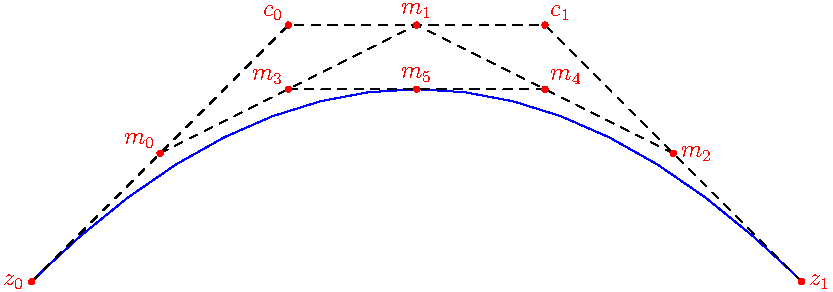
\includegraphics[scale=1]{imagens/capitulo5/bezier2.pdf}
	\caption{Ilustração do algoritmo recursivo de subdivisão de curvas de Bézier.}
	\label{fig:beziersub}
\end{figure}

O Código \ref{cod:asymptote} mostra os comandos em Asymptote usados para gerar a Figura \ref{fig:beziersub}. Note como é simples e intuitivo desenhar retas e posicionar os nomes dos pontos, e a definição da função auxiliar \texttt{midpoint}. 

\begin{listing}[ht]
	\begin{minted}[linenos=true, autogobble, bgcolor=Cornsilk1]{asy}
	import beziercurve;

	pair midpoint(pair a, pair b) {return interp(a,b,0.5);}

	pair m0=midpoint(z0,c0);
	pair m1=midpoint(c0,c1);
	pair m2=midpoint(c1,z1);

	draw(m0--m1--m2,dashed);
	dot("$m_0$",m0,NW,red);
	dot("$m_1$",m1,N,red);
	dot("$m_2$",m2,red);

	pair m3=midpoint(m0,m1);
	pair m4=midpoint(m1,m2);
	pair m5=midpoint(m3,m4);

	draw(m3--m4,dashed);
	dot("$m_3$",m3,NW,red);
	dot("$m_4$",m4,NE,red);
	dot("$m_5$",m5,N,red);
	\end{minted}
	\caption{Código Asymptote usado para gerar a Figura \ref{fig:beziersub}.}
	\label{cod:asymptote}
\end{listing}



O Asymptote também permite que se construa animações dos gráficos gerados usando seu pacote \texttt{animation}\index{animation}, que empilha múltiplas imagens em um \gls{gif}\index{GIF} animado ou um vídeo \gls{mpeg}\index{MPEG} usando o programa \texttt{convert} do software ImageMagick. Assim como no caso do Ti\textit{k}Z, essas animações só podem ser visualizadas em leitores de \gls{pdf}\index{PDF} que suportem JavaScript\index{JavaScript} ou em browsers.

O Asymptote provê uma interface gráfica bem simples, a \texttt{xasy}\index{xasy}, que permite que se veja imediatamente o resultado da manipulação dos elementos gráficos. Como a interface não é tão completa, o usuário pode preferir salvar o código do gráfico e completar a programação fora da ferramenta.

Uma boa referência inicial é o tutorial disponível em \url{https://asymptote.sourceforge.io/asymptote_tutorial.pdf} \parencite{asymptotetut}. Caso precise de informações mais detalhadas, você pode acessar o manual do Asymptote\index{Asymptote} em \url{http://mirrors.ctan.org/graphics/asymptote/doc/asymptote.pdf} \parencite{asymptote}. Finalmente, você também pode obter o cartão de referência dos comandos Asymptote no endereço \url{http://mirrors.ctan.org/graphics/asymptote/doc/asyRefCard.pdf} \parencite{asymptoterefcard}. 





% Capitulo 5: Proposta de ferramenta
\chapter{Proposta de Ferramenta}

Nesta seção, será apresentada uma ferramenta cujo objetivo é automatizar a geração de questões, com o objetivo de tornar mais fácil a construção e geração de questões. A ferramenta baseia-se em um modelo de separação entre duas entidades principais : (i) um JSON de template, responsável por definir a estrutura geral das questões; e (ii) um JSON de questões, que instancia as variações específicas de cada problema. O sistema foi planejado para permitir que os professores sejam responsáveis pela elaboração e manutenção dos templates. Por outro lado os usuários estudantes interagem apenas com as questões geradas a partir desses templates.

\section{JSON de Templates}

O primeiro componente é o JSON de Template, ilustrado na Figura \ref{fig:json-de-templates}, no qual o enunciado geral (\textit{cabeçalho}) descreve a estrutura padrão que será aplicada em todas as questões derivadas. Nele, é definido as partes fixas do enunciado e a forma como os elementos variáveis serão combinados para formar a questão. Em seguida, cada categoria de variáveis contém uma lista de opções textuais ou numéricas que podem assumir diferentes valores de acordo com a necessidade, permitindo a criação de múltiplas versões de um mesmo problema.


\begin{figure}[ht]
	\centering
	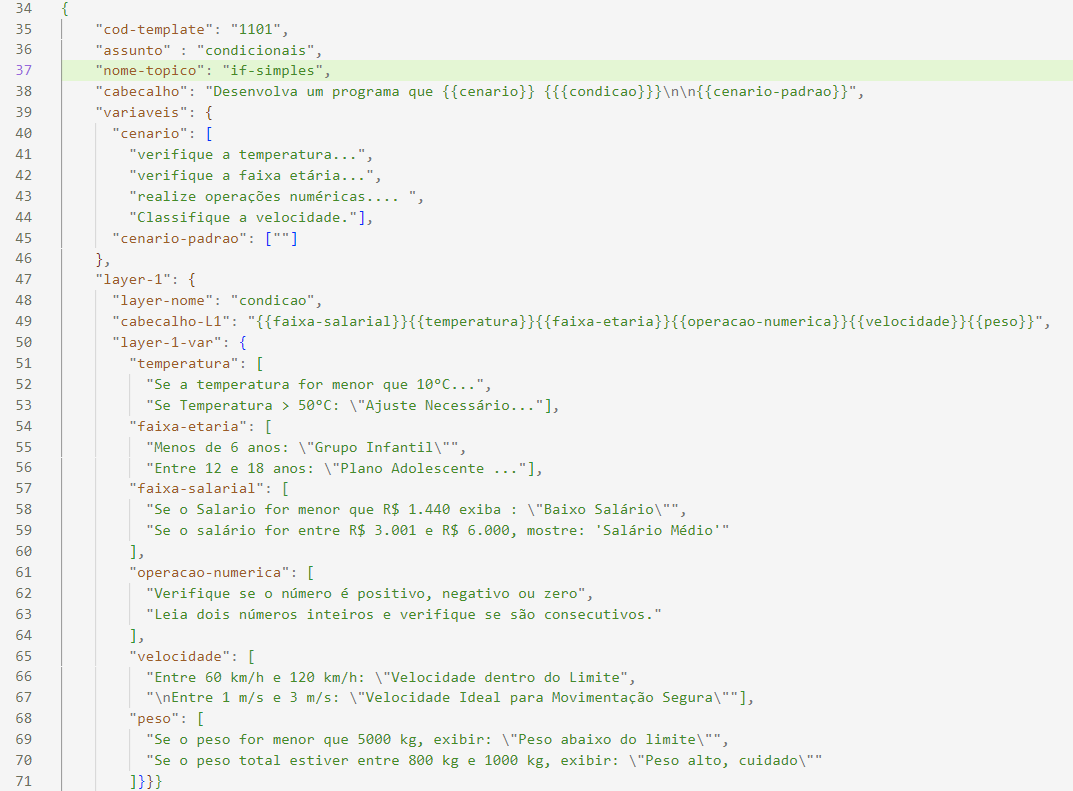
\includegraphics[width=16cm]{./imagens/capitulo7/json-de-template}
	\caption{JSON de Templates (Elaboração própria, 2025) }
	\label{fig:json-de-templates}
\end{figure}
\section{JSON de Questões}

O segundo componente é o JSON de Questões, ilustrado na figura \ref{fig:json-de-questoes}, cujo objetivo é definir o formato final de cada questão que será efetivamente apresentado aos estudantes. Neste arquivo, cada questão é identificada por um código, um título e um mapeamento dos índices das variáveis que aponta para as categorias estabelecidas no template. Assim, essa estrutura não precisa carregar toda formatação do template, apenas fazer referência aos elementos já definidos no arquivo de templates. Dessa forma, não é necessário carregar toda formatação do enunciado em cada questão, mas apenas fazer referencia ao índice dos elementos definidos do JSON de Templates. Essa separação favorece a reutilização do mesmo modelo em diversas situações, bastando alterar os atributos de cada problema conforme necessário.

\begin{figure}[ht]
	\centering
	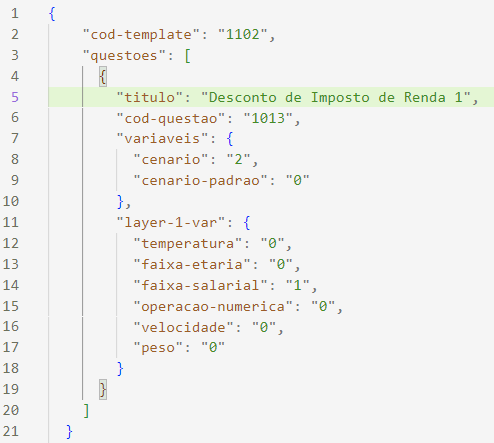
\includegraphics[width=12cm]{./imagens/capitulo7/json-de-questoes}
	\caption{JSON de Questões (Elaboração própria, 2025) }
	\label{fig:json-de-questoes}
\end{figure}
Na próxima seção serão discutidos os aspectos de implementação, apresentando a ferramenta utilizada e como a geração de questões pode ser aplicada na prática, como os dados dos arquivos JSON são processados para gerar as questões, bem como um panorama geral do sistema e detalhes do \textit{prompt} utilizado pela IA.

\section{Ferramenta}

Segundo \parencite{martin2017} a arquitetura de software deve representar o domínio do sistema, e não apenas dos \textit{frameworks} ou tecnologias empregadas. com base neste principio, a Figura \ref{fig:modelo-arquitetural} organiza o sistema em quatro camadas: Apresentação, Aplicação, Domínio e Infraestrutura — refletindo o fluxo de execução do sistema.

\begin{figure}[ht]
	\centering
	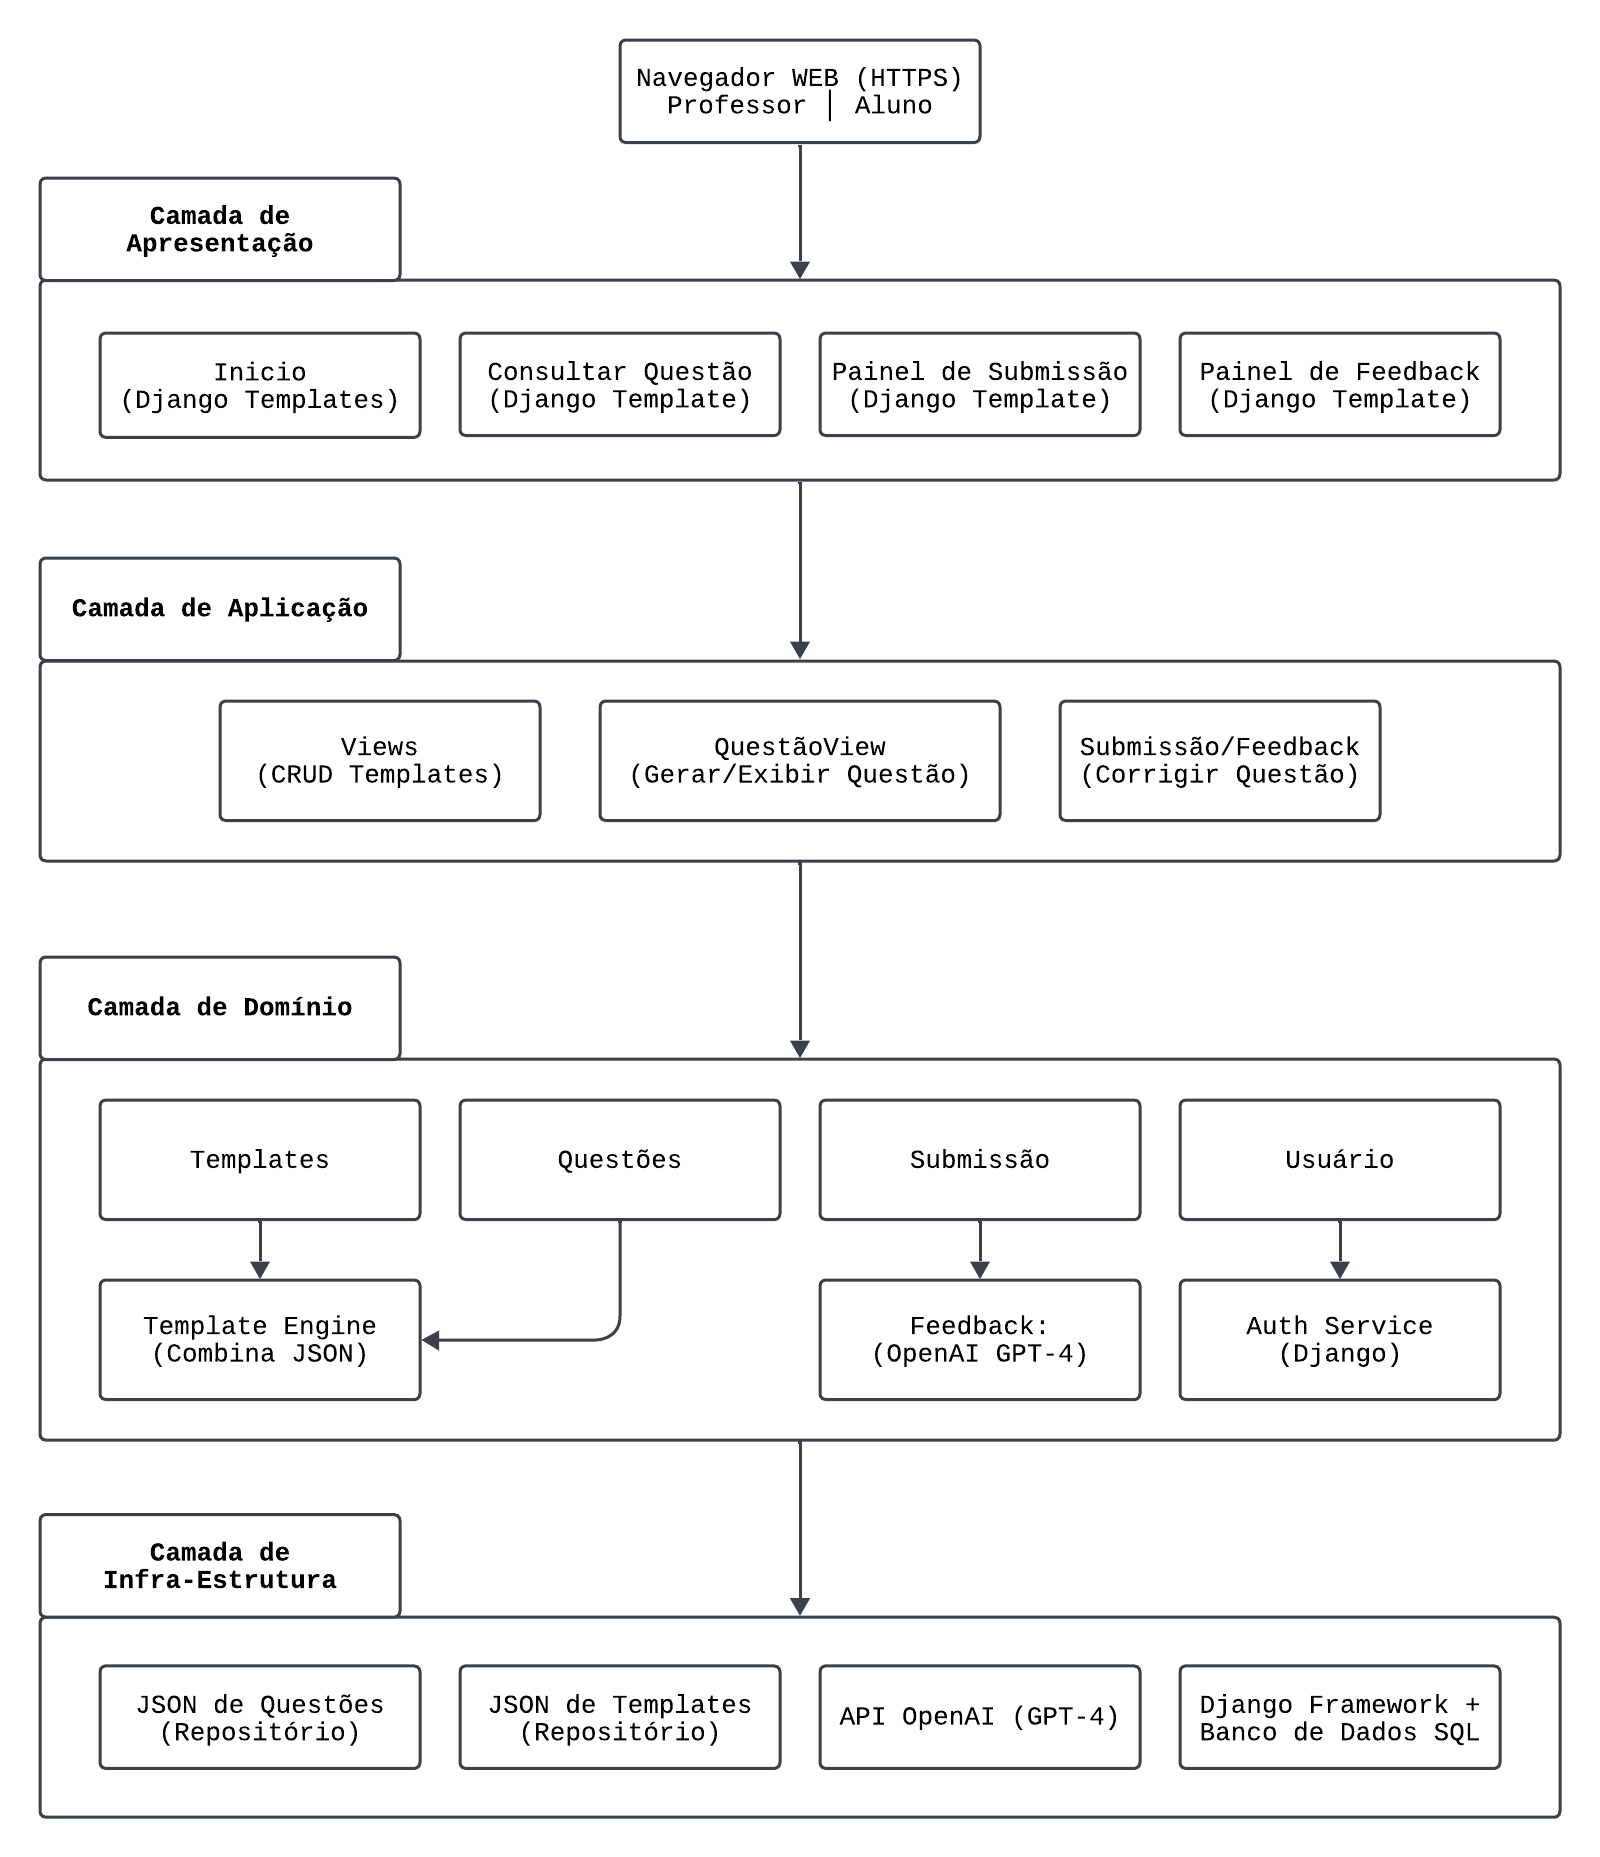
\includegraphics[width=12cm]{./imagens/capitulo7/modelo-arquitetural}
	\caption{Modelo arquitetural do sistema (Elaboração própria, 2025) }
	\label{fig:modelo-arquitetural}
\end{figure}



A ferramenta utilizada foi o \textit{Arena Code}, desenvolvida pelo autor desta pesquisa para a geração automática de questões de programação. O código-fonte da aplicação encontra-se disponível nas referências \parencite{arena-code}.
As figuras a seguir ilustram o ciclo de uso da ferramenta, no qual cada interface exerce funções específicas em diferentes momentos da interação entre o usuário e o sistema. A janela da página inicial, apresentada na Figura \ref{fig:modelo-arquitetural}, exibe uma síntese dos templates disponíveis : assunto, dificuldade e número total de combinações geradas. 
Ao selecionar um assunto de interesse, como por exemplo estruturas condicionais na Figura  \ref{fig:ferramenta-topicos}, o sistema gera dinamicamente uma questão relacionada ao tema escolhido. Essa geração é basada em um template multicamadas, que permite combinar diferentes cenários dentro de uma mesma tabela, ou utilizar mútilas tabelas para um único cenário. Essa abordagem amplia consideravelmente a quantidade de variações possíveis para uma mesma estrutura de template. 
\begin{figure}[H]
  \centering
  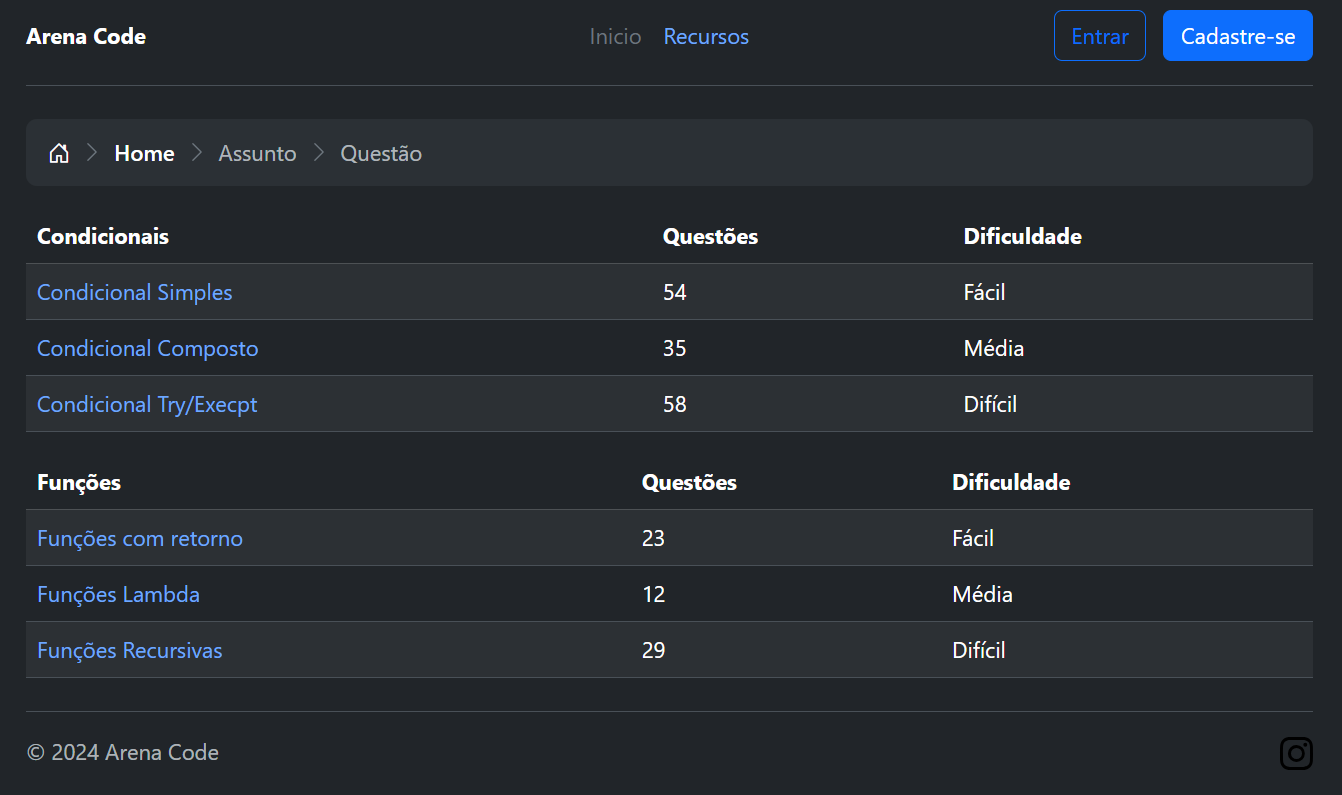
\includegraphics[width=\textwidth]{./imagens/capitulo7/ferramenta-fig1}
  \caption{Página inicial com lista de assuntos (Elaboração própria, 2025)}\label{fig:ferramenta-topicos}
\end{figure}


O processo tem início com a seleção de um template que reúne uma lista de variações previamente estruturadas. A partir dessa escolha, o sistema combina os elementos correspondentes e gera dinamicamente uma questão, que é apresentada ao aluno na página seguinte conforme a Figura \ref{fig:ferramenta-enunciado}.  Na página do enunciado, a esquerda será exibido a questão gerada de acordo com o assunto do template selecionado, e à direita é exibido o editor de código, onde o estudante deve escrever a solução proposta e posteriormente acionar o botão \textbf{"submeter código"}, o aluno será redirecionado para página de feedback. 

\begin{figure}[H]
  \centering
  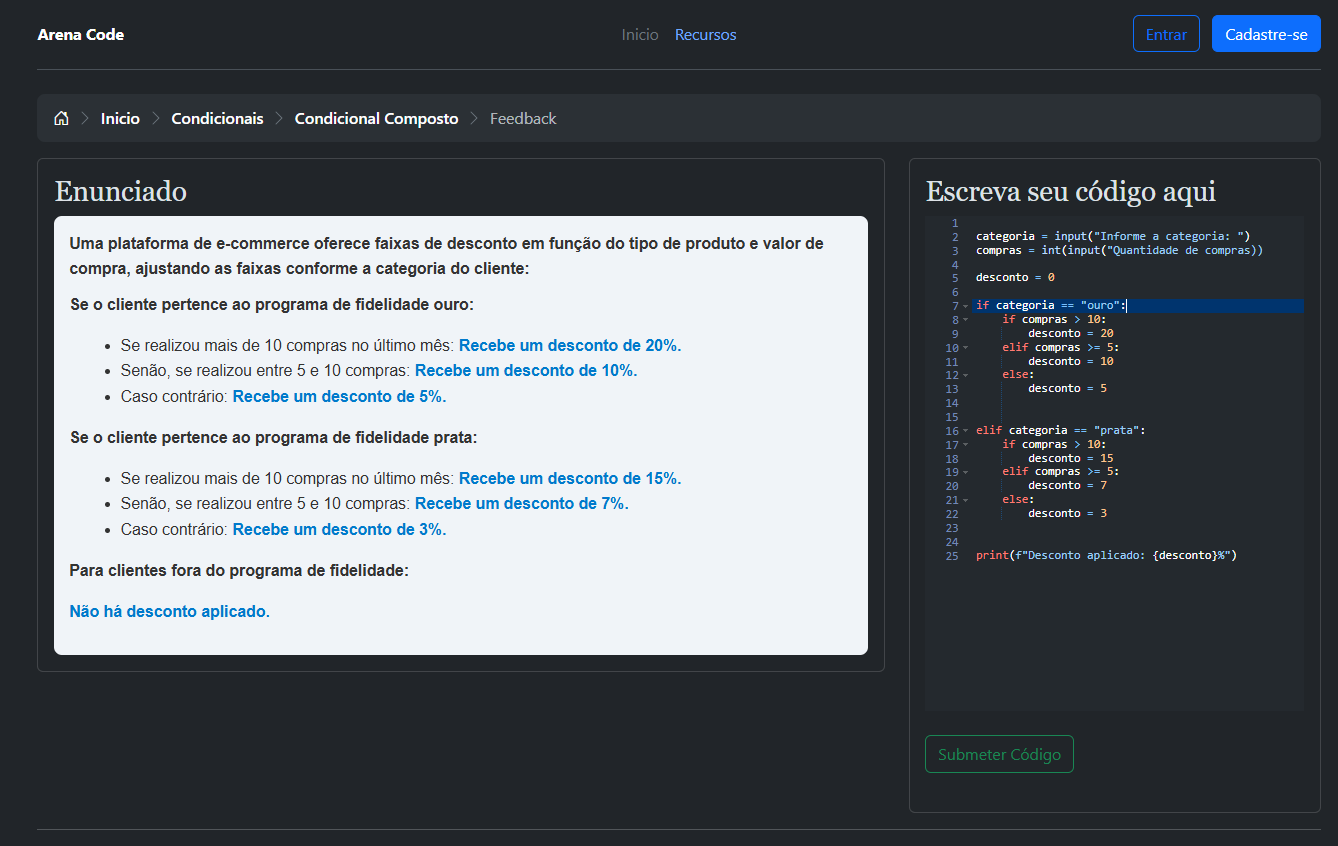
\includegraphics[width=\textwidth]{./imagens/capitulo7/ferramenta-fig2}
  \caption{Tela de resolução: Enunciado e editor de código.  (Elaboração própria, 2025)}\label{fig:ferramenta-enunciado}
\end{figure}

A flexibilidade desse template faz com que seja possível criar muitas variações de exercícios, cada um abordando aspectos distintos das estruturas condicionais. Em seguida, o código escrito no ambiente de resolução oposto e submetido para avaliação. Para realizar a correção, a ferramenta usa uma \gls{api} da OpenAI, que utiliza o GPT-4 para verificar os casos de teste associados ao problema e devolve um feedback  sobre a resposta enviada. Essa estratégia incentiva o aprimoramento constante do aluno, pois o mesmo pode corrigir e reenviar sua solução quantas vezes forem necessárias até alcançar o resultado desejado. 

\begin{figure}[ht]
	\centering
	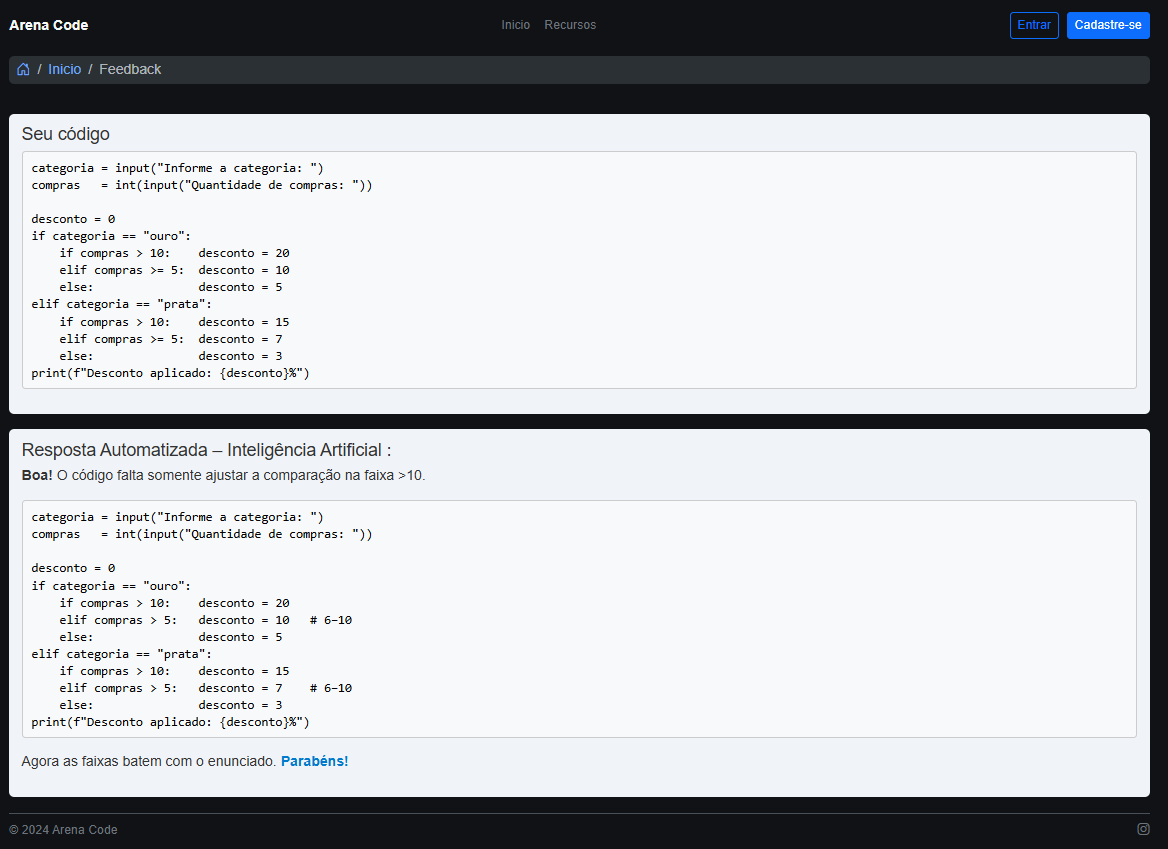
\includegraphics[width=14cm]{./imagens/capitulo7/ferramenta-fig3}
	\caption{Tela de Feedback (Elaboração própria, 2025) }
	\label{fig:ferramenta-fedback}
\end{figure}


Para realizar essa análise, a ferramenta monta um prompt com apenas duas entradas : o enunciado da questão e o código submetido. E posteriormente envia ao GPT-4. O modelo executa os casos de testes, identifica eventuais erros e devolve um feedback ao aluno. Esse ciclo tem como objetivo promover o aprimoramento contínuo, pois o aluno pode revisar e reenviar sua solução quantas vezes forem necessárias até alcançar o resultado desejado.  Para torná-lo utilizável pela interface, o sistema executa o seguinte prompt: 

\subsubsection{Entradas}

\begin{itemize}
    \item \textbf{Questão}: Enunciado da questão de programação que o estudante deve resolver.
    \item \textbf{Código submetido}: Código-fonte enviado pelo estudante como tentativa de solução.
\end{itemize}

\subsubsection{Prompt Enviado ao API do ChatGPT:}

"Você é um assistente especializado em revisar código e dar feedback aos alunos. Se minha resposta estiver errada explique exatamente onde errei, baseado na [\textbf{Questão}] e no [\textbf{Código submetido}], corrija a resposta de forma didática e dê uma resposta detalhada."


\section{Vantagens e limitações do modelo multicamadas}

Embora a configuração inicial dos templates exija um certo esforço de elaboração, esse investimento é compensado pela possibilidade de reutilizar as questões em diversas situações, reduzindo a necessidade de criar novos problemas para cada turma ou semestre. Uma vez que o repositório de problemas e cenários esteja consolidado, os professores podem extrair diferentes conjuntos de exercícios de forma rápida, adequando-os a diferentes turmas, níveis de dificuldade ou contextos de aplicação. A prática frequente com casos variados também permite aos estudantes um aprendizado mais consistente, pois eles entram em contato com diversas nuances do uso das estruturas condicionais, refinando sua capacidade de resolução de problemas, isto também se aplica a todo contexto que seja possível incluir vários cenários diferentes para um mesmo problema. No entanto, a mesma particularidade que torna o modelo efetivo também introduz algumas dificuldades tais como a manutenção de múltiplas camadas pode ser complexa sem ferramentas de apoio, e a qualidade das respostas depende diretamente da clareza dos \emph{prompts}. Para resumir esses pontos, a Tabela~\ref{tab:beneficios-limitacoes} apresenta um comparativo entre os principais benefícios observados e as limitações identificadas durante o desenvolvimento deste trabalho.


\begin{table}[H]
\centering
\caption{Comparativo de benefícios e limitações do modelo multicamadas}
\label{tab:beneficios-limitacoes}
\begin{tabular}{|p{7cm}|p{7cm}|}
\hline
\textbf{Benefícios} & \textbf{Limitações / Dificuldades} \\ \hline
\begin{itemize}[leftmargin=*]
    \item \textbf{Reutilização eficiente:} um único template pode gerar centenas de variações, reduzindo o esforço contínuo de elaboração de novos exercícios.%
    \item \textbf{Escalonamento:} permite calibrar o nível de dificuldade ou o contexto sem recriar todo o enunciado, respondendo rapidamente a diferentes perfis de turma.%
    \item \textbf{Facilita a manutenção:} ajustes conceituais (erros, melhorias, mudança de nomenclatura) são feitos apenas no template central.%
    \item \textbf{Feedback em tempo real:} integração direta com \textit{APIs} de IA (GPT-4) fornece correções detalhadas e adaptativas, incentivando múltiplas tentativas.%
    \item \textbf{Clareza para o professor:} separação explícita entre \emph{estrutura} e \emph{instâncias} torna o repositório de questões mais organizado e auditável.%
\end{itemize} &
\begin{itemize}[leftmargin=*]
    \item \textbf{Curva de aprendizagem inicial:} modelar corretamente as camadas demanda planejamento e domínio de variáveis, o que pode desestimular docentes sem familiaridade com templates.%
    \item \textbf{Ausência de interface gráfica:} editar arquivos JSON manualmente é suscetível a erros de sintaxe e aumenta o tempo de configuração; uma GUI dedicada ainda é necessária.%
    \item \textbf{Depuração complexa:} quando múltiplas camadas interagem, localizar inconsistências (e.g.\ índices trocados) pode ser trabalhoso.%
    \item \textbf{Limitações de mídia:} o modelo funciona muito bem para textos e números, mas não lida igualmente bem com variações de imagens, exigindo adaptações extras.%
    \item \textbf{Dependência de \textit{prompts} precisos:} erros na formulação do prompt para o GPT-4 geram feedback incoerente; não há controle total sobre a aleatoriedade das respostas.%
\end{itemize} \\ \hline
\end{tabular}
\end{table}


Com esse resultado podemos responder parcialmente à \textbf{QP1}. Esses pontos formam a base para o capítulo seguinte, onde será apresentado um estudo de caso com professores que ensinam programação, e como as vantagens se concretizam na prática e até que ponto os desafios podem ser amenizados. Só então será possível responder totalmente à \textbf{QP1} e \textbf{QP3}, avaliando o impacto real desta abordagem.


  
  % Capitulo 6: Sexto capítulo (arquivo capitulos/capitulo6.tex)
  %% Capítulo 6
\chapter{Correções}\label{cap:correcoes}

Durante a escrita de uma dissertação ou tese, é importante que os orientadores possam sinalizar correções e comentar trechos de texto, figuras, tabelas e outros elementos. Isto pode ser feito por anotações feitas diretamente no arquivo \gls{pdf}\index{PDF} ou usando um pacote que implemente marcações de correções.

Neste modelo, selecionamos o pacote \texttt{changes}\index{changes} para este fim. O pacote \texttt{changes} permite que se notifique mudanças no documento com identificação do indivíduo que as fez, facilitando a comunicação quando mais de duas pessoas estão alterando o documento.

O Código \ref{cod:changes-setup} descreve os comandos usados para configurar o pacote para funcionar com este documento, definindo os nomes dos usuários que irão interagir com o documento e o modo atual do documento, o \texttt{draft}\index{draft}.

\begin{listing}[ht]
	\begin{minted}[linenos=true, autogobble, bgcolor=Cornsilk1]{tex}
	\usepackage[draft,markup=underlined]{changes}
	\definechangesauthor[name={Bruno},color=violet]{Bruno}
	\definechangesauthor[name={Hari},color=purple]{Hari}
	\definechangesauthor[name={Salvor},color=olive]{Salvor}
	\end{minted}
	\caption{Código \LaTeX{} usado para definir as informações referentes ao pacote \texttt{changes}.}
	\label{cod:changes-setup}
\end{listing}

O pacote \texttt{changes}\index{changes} permite que se altere da versão \texttt{draft}\index{draft}, que exibe os comentários e mudanças, para a versão \texttt{final}\index{final} com a alteração de apenas um comando, trocando a Linha 1 do Código \ref{cod:changes-setup} pela linha do Código \ref{cod:changes-final}. 

\begin{listing}[ht]
	\begin{minted}[linenos=true, autogobble, bgcolor=Cornsilk1]{tex}
		\usepackage[final]{changes}
	\end{minted}
	\caption{Código \LaTeX{} usado para definir o formato do documento como \texttt{final} ao invés de \texttt{draft} com relação ao pacote \texttt{changes}.}
	\label{cod:changes-final}
\end{listing}

Na primeira definição mostrada, usamos o parâmetro \texttt{draft}\index{draft}, indicando que a versão atual do documento mostrará os comentários e mudanças, e a parâmetro \texttt{markup}\index{markup} com o estilo \texttt{underlined}\index{underlined} associado a ele. Os estilos de \texttt{markup} (marcação) disponíveis são: 

\begin{itemize}
	\item \texttt{default}\index{default} - marcação padrão para comentários e textos adicionados, deletados e destacados;
	\item \texttt{underlined}\index{underlined} - sublinhado para textos adicionados, sublinhado ondulado para textos destacados, e padrão para textos deletados e comentários;
	\item \texttt{bfit}\index{bfit} - negrito para textos adicionados, itálico para textos deletados, e padrão para textos deletados e comentários;
	\item \texttt{nocolor}\index{nocolor} - sem cores para marcações, sublinhado para textos adicionados, sublinhado ondulado para textos destacados, e padrão para textos deletados e comentários;
\end{itemize}

O pacote ainda permite que você defina individualmente o estilo de marcação para cada um dos quatro tipos de alterações disponíveis. Para mais detalhes, consulte o manual do pacote. \comment[id=Bruno]{Os comentários no estilo \texttt{todo} ficam localizados na borda do documento.}

Os cinco comandos usados para efetuar mudanças e fazer comentários são apresentados com exemplos simples.
\begin{itemize}
	\item \textbackslash \texttt{added}\index{added} - Marca textos adicionados. \added[id=Hari]{Adicione isso porque é necessário.} O Código \ref{cod:changes-added} mostra como isso foi feito.
	\begin{listing}[ht]
		\begin{minted}[linenos=true, autogobble, bgcolor=Cornsilk1]{tex}
		\added[id=Hari]{Adicione isso porque é necessário.}
		\end{minted}
		\caption{Código do \texttt{changes} usado para sugerir a adição de texto.}
		\label{cod:changes-added}
	\end{listing}

	\item \textbackslash \texttt{deleted}\index{deleted} - Marca textos deletados. \deleted[id=Salvor]{Texto removido porque estava errado.} O Código \ref{cod:changes-deleted} mostra como isso foi feito.
	
	\begin{listing}[ht]
		\begin{minted}[linenos=true, autogobble, bgcolor=Cornsilk1]{tex}
		\deleted[id=Salvor]{Texto removido porque estava errado.}
		\end{minted}
		\caption{Código do \texttt{changes} usado para sugerir a remoção de texto.}
		\label{cod:changes-deleted}
    \end{listing}

	\item \textbackslash \texttt{replaced}\index{replaced} - Marca textos deletados e suas reposições. \replaced[id=Hari]{Importante para que se visualize sugestões de correções de texto.}{Não é importante.} O Código \ref{cod:changes-replaced} mostra como isso foi feito.
	
	\begin{listing}[ht]
		\begin{minted}[linenos=true, autogobble, bgcolor=Cornsilk1]{tex}
		\replaced[id=Hari]{Importante para que se visualize sugestões de 
		correções de texto.}{Não é importante.}
		\end{minted}
		\caption{Código do \texttt{changes} usado para sugerir a troca de texto.}
		\label{cod:changes-replaced}
	\end{listing}

	\item \textbackslash \texttt{highlight}\index{highlight} - Destaca trechos de texto \highlight[id=Bruno]{como este aqui.} O Código \ref{cod:changes-highlighted} mostra como isso foi feito.
	
	\begin{listing}[ht]
		\begin{minted}[linenos=true, autogobble, bgcolor=Cornsilk1]{tex}
			\highlight[id=Bruno]{como este aqui.}
		\end{minted}
		\caption{Código do \texttt{changes} usado para destacar texto.}
		\label{cod:changes-highlighted}
	\end{listing}

	\item \textbackslash \texttt{comment}\index{comment} - Cria um comentário e coloca-o no documento de acordo com a opção definida. Neste caso, estamos usando a opção \texttt{todo}, como visto no comentário inserido acima.\comment[id=Bruno]{Veja o manual do pacote \texttt{changes} para ver as outras opções.} O Código \ref{cod:changes-comment} mostra como isso foi feito.
	
	\begin{listing}[H]
		\begin{minted}[linenos=true, autogobble, bgcolor=Cornsilk1]{tex}
		\comment[id=Bruno]{Veja o manual do pacote \texttt{changes} para ver as 
		outras opções.}
		\end{minted}
		\caption{Código do \texttt{changes} usado para destacar texto.}
		\label{cod:changes-comment}
	\end{listing}

\end{itemize}

É importante frisar que comentários podem ser incluídos nos outros quatro comandos. \added[id=Hari, comment={Veja no manual.}]{Inclua exemplo.} Os comandos usados para fazer tal alteração podem ser vistos no Código \ref{cod:changes-comment-added}.

\begin{listing}[ht]
	\begin{minted}[linenos=true, autogobble, bgcolor=Cornsilk1]{tex}
		\added[id=Hari, comment={Veja no manual.}]{Inclua exemplo.}
	\end{minted}
	\caption{Código do \texttt{changes} que mostra um comentário dentro de um comando de adição.}
	\label{cod:changes-comment-added}
\end{listing}

No sítio \gls{ctan}\index{CTAN} existem dois manuais para o pacote \texttt{changes}\index{changes}, um sem o código fonte do pacote (\url{http://mirrors.ctan.org/macros/latex/contrib/changes/changes.english.pdf}) \parencite{changes} e outro com o código fonte (\url{http://mirrors.ctan.org/macros/latex/contrib/changes/changes.english.withcode.pdf}).


% Capitulo 7: Estudo de Caso
\chapter{Estudo de Caso}

Este capítulo apresenta o estudo de caso conduzido com professores de \textit{introdução à programação} com o objetivo de investigar a viabilidade, utilidade prática e os desafios associados ao uso de templates multicamadas proposto neste trabalho. A pesquisa adota uma abordagem integrada à pesquisa-ação, com uso de métodos mistos (quantitativos e qualitativos). O estudo foi conduzido e estruturado para oferecer evidências que respondem às três questões de pesquisa (QP1, QP2 e QP3) conforme as diretrizes metodológicas recomendadas pela \gls{ceie} para estudos de caso.

\section{Objetivo do Estudo}
O objetivo deste estudo de caso é investigar a aplicabilidade da geração automática de questões utilizando templates multicamadas no contexto do ensino de programação, com base na experiência de professores na construção desses templates, e em suas percepções sobre a utilidade e os desafios da abordagem. Para isso, são apresentados a abordagem utilizada,  os procedimentos envolvidos e as métricas adotadas, que fundamentam a coleta e análise dos dados qualitativos e quantitativos que serão discutidos nas seções seguintes.
Embora não tenha sido possível aplicar o feedback automatizado aos participantes devido ao tempo limitado para o desenvolvimento deste estudo, a literatura  indica que este recurso tem potencial significativo para contribuir no aprendizado, como evidenciado por trabalhos como o de \parencite{vanpraet2024} e \parencite{fung2024} indicam que a incorporação de feedback automatizado se utilizado corretamente pode aumentar de forma significativa o desempenho dos estudantes.

\section{Metodologia do Estudo de Caso}

Este estudo adotou uma abordagem mista que combina técnicas quantitativas e qualitativas dentro de um ciclo de pesquisa. A opção por integrar essas abordagens decorreu de duas necessidades complementares: mensurar, de forma objetiva, o tempo gasto, o número de questões produzidas e a taxa de reaproveitamento dos \textit{templates}, ao mesmo tempo em que se investigavam as percepções, dificuldades e sugestões dos professores, o processo foi divido em cinco etapas que são:  

\begin{enumerate}
    \item \textbf{Apresentação da proposta}:  Foi exibido um vídeo curto dividido em três blocos: (direcionamento, questões base e estrutura do modelo) com explicações sobre os fundamentos da geração automática de questões usando templates multicamadas, além de orientações de uso e exemplos práticos de aplicação. O objetivo foi garantir  compreensão do assunto por parte dos professores.
    
    \item \textbf{Criação de templates pelos professores}:  Os professores participantes após apresentação do modelo vão elaborar os templates utilizando uma estrutura previamente definida. A orientação fornecida foi divida em três tópicos principais:
    \begin{itemize}
        \item \textbf{Direcionamento} : fundamentos e exemplos com perguntas-chave para ajudar na formulação do enunciado e identificação dos elementos variáveis.
        \item \textbf{Questões base} : Orientações para identificar os aspectos fundamentais do problema que desejam transformar em uma questão.
        \item \textbf{Estrutura modelo} : Um guia de construção do template, indicando com organizar o template, variáveis e condições.
    \end{itemize}

Os professores puderam utilizar ferramentas de auxilio como o \gls{chatgpt}, para ajudar na criação e sugestão de variações e contextos. Esse suporte tem como objetivo facilitar a criação dos templates, ampliar as possibilidades de formulação e oferecer templates mais adaptáveis.

    \item \textbf{Objetivos do Estudo}:  O objetivo geral deste estudo é avaliar a aplicabilidade da utilização de templates multicamadas na geração automática de questões de programação, com base na experiência prática dos professores envolvidos no processo. Os objetivos específicos que orientam este estudo são:

       \begin{itemize}
        \item \textbf{Medir a viabilidade operacional} : Considerando o tempo necessário, o esforço envolvido e nível de sucesso na criação das questões a partir dos templates.
        \item \textbf{Verificar a utilidade prática} : Analisando a economia de tempo, a diversidade das questões geradas e o nível de engajamento do professor.
        \item \textbf{Identificar dificuldades} : Analisar aspectos relacionados à curva de aprendizagem, à definição e ao uso adequado de variáveis, bem como as possíveis barreiras técnicas encontradas durante a construção dos templates. 
    \end{itemize}
    
    \item \textbf{Perfil dos Professores}:  Para garantir que os resultados reflitam um panorama representativo dos professores de Introdução a programação, foi definido critérios de inclusão e coleta de informação de para cada professor com base nos seguintes aspectos: 
    \begin{itemize}
        \item \textbf{Experiência recente} : lecionam ou lecionaram disciplinas introdutórias de programação em pelo menos 2 semestres nos cinco anos anteriores ao estudo. 
        \item \textbf{Disponibilidade} : Compromisso para criar e avaliar templates e responder a entrevista.
    \end{itemize}

    \item \textbf{Variáveis levantadas pelo questionário}:  O formulário (vide anexo A  (\ref{cap:anexos}) ) foi dividido em blocos, cada um mapeando uma questão de pesquisa: 

\begin{table}[htbp]
    \centering
    \renewcommand{\arraystretch}{1.3}
    \begin{tabular}{|p{4cm}|p{5.4cm}|p{6cm}|}
        \hline
        \textbf{Bloco} & \textbf{Variáveis coletadas} & \textbf{Objetivo} \\ \hline
        Perfil profissional & Titulação, anos de docência, linguagens mais ensinadas. & Relacionar experiência ao \textbf{tempo médio} de criação de templates. \\ \hline
        Prática com templates & Tempo gasto, número de questões geradas, taxa de reaproveitamento. & Medir \textbf{viabilidade} e \textbf{utilidade} operacional. \\ \hline
        Percepções e desafios & Dificuldades encontradas, contribuição percebida, preferências de uso. & Identificar \textbf{barreiras} técnicas e pedagógicas. \\ \hline
        Adaptação de questões existentes & Grau de facilidade em converter questões próprias para o formato multicamada. & Verificar \textbf{capacidade de transformação} sem suporte externo. \\ \hline
    \end{tabular}
    \caption{Estrutura do questionário (Elaboração própria, 2025)}
    \label{tab:questionario-objetivos}
\end{table}



    
    \begin{itemize}
        \item \textbf{Questionário olline (anexo A)} 
        \item \textbf{Video Tutorial (Roteiro no Anexo B)} :
        \item \textbf{Guia de construção de templates com exemplos} 
        \item  \textbf{Avaliação da qualidade dos templates} 
    \end{itemize}



    \item \textbf{Métricas e indicadores}:  Estr
    \begin{itemize}
        \item \textbf{Tempo médio pra criar um template} 
        \item \textbf{Numero de questões geradas por template} :
        \item \textbf{Taxa de reaproveitamento} 
        \item  \textbf{Sucesso em converter a questão existende em template} 
    \end{itemize}

    
\end{enumerate}






\section{Resultados Observados}

O estudo revelou que os professores conseguiram elaborar templates funcionais e diversificados, utilizando as orientações fornecidas. No entanto, alguns desafios foram identificados:

\begin{enumerate}
    \item \textbf{Dificuldade Inicial}: Professores com menor familiaridade com conceitos de questões baseada em templates demonstraram dificuldades em identificar elementos variáveis e combinar os valores.
    \item \textbf{Uso da IA Gnerativa} : A integração do ChatGPT foi bem recebida, e os participantes relataram que as sugestões fornecidas pela ferramenta ajudaram na proposta de contextos diversificados.
    \item \textbf{Percepção Geral} : Os professores consideraram o modelo útil para reduzir o tempo de elaboração de questões, no entanto preferiram que os templates já estivessem prontos pra utilizar, e após construídos pudessem acrescentar ou editar a estrutura conforme a necessidade ao invés de criar do zero.
\end{enumerate}


\section{Beneficios e Desafios Percebidos}

redução do esfoço de elaboração, maior diversidade de exercicio

identificar corretamente as variaveis e seus valores
curva de aprendizagem para manipular o template
preferencia em usar templates-base prontos em vez de começar do zero.

\section{Considerações Finais do Estudo de Caso}
A aplicação foi realizada com um número reduzido de professores, o que limita a generalização dos resultados. Estudos futuros poderão expandir o alcance para incluir mais participantes para validar a proposta. Apesar das limitações, a abordagem de geração automática de questões demonstrou um potencial significativo para criar questões em escala e reduzir o esforço necessário para a construção de conteúdos por parte dos professores.


RESPOSTA AS QUESTÕES DE PESQUISA COM OS INDICADORES 
VIABILIDADE : INDICADOR DE TEMPO
UTILIDADE : TAXA DE APROVEITAMENTO 
DESAFIOS : FALTA DE MODELOS PRÉ-PRONTOS

AMOSTRA REDUZIDA LIMITA A GENERALIZAÇÃO



\paragraph{\textbf{Principais Desafios Identificados}}

\begin{itemize}
    \item \textbf{Curva de aprendizagem inicial} (especialmente na identificação de variáveis e condições);
    \item \textbf{Necessidade de modelos‐base} para acelerar a adoção;
    \item \textbf{Integração com sistemas de avaliação existentes} (Moodle, Google Forms, etc.), que exigirá conversores automáticos — apontado como trabalho futuro.
\end{itemize}
\textbf{QP3 – Desafios:} maior dificuldade em definir variáveis e preferências por templates‐base prontos; 60 \% solicitaram um repositório inicial de modelos. 

  % Capitulo 7: Sétimo capítulo (arquivo capitulos/capitulo7.tex)
   %% Capítulo 7
\chapter{Referências}\label{cap:refs}

O pacote \texttt{hyperref}\index{hyperref} \parencite{hyperref} estende a funcionalidade de todos os comandos que implementam referências cruzadas do \LaTeX{}, como sumário, bibliografia, listas de figuras e tabelas, para produzir comandos especiais que geram \textit{links} de hipertexto. O pacote permite ainda a criação de \textit{links} para documentos externos e URLs.

O Código \ref{cod:hyperref} mostra os comandos usados para carregar o pacote \texttt{hyperref}, com as opções \texttt{colorlinks}\index{colorlinks}, que colore os \textit{links} das referências, \texttt{hyperindex}\index{hyperindex}, que indica que o índice deve conter \textit{hyperlinks}\index{hyperlinks}, \texttt{plainpages=false}\index{plainpages}, que força que as âncoras das páginas sejam nomeadas em números arábicos,  \texttt{pdfusetitle}\index{pdfusetitle}, que lê as informações de título, autor, etc. e as adiciona ao arquivo \gls{pdf}\index{pdf}, e
\texttt{pdflang=pt-BR}\index{pdflang}, que identifica a linguagem do documento como sendo Português do Brasil. O segundo comando, na Linha 3, associa informações aos campos que serão lidos pelo pacote \texttt{hyperref}\index{hyperref}, caso a opção \texttt{pdfusetitle}\index{pdfusetitle} esteja ativa, e associados aos campos de informação do arquivo \gls{pdf}\index{pdf}.

\begin{listing}[ht]
	\begin{minted}[ linenos=true, autogobble, bgcolor=Cornsilk1 ]{tex}
	\usepackage[colorlinks, hyperindex, plainpages=false, pdfusetitle, 
	pdflang=pt-BR]{hyperref} 
	\hypersetup{pdftitle={Modelo PPgSC de Dissertações e Teses em LaTeX}, 
	pdfauthor={Bruno Motta de Carvalho}, 
	pdfsubject={Manual do modelo LaTeX do PPgSC-UFRN},
	pdfkeywords={LaTeX, diagramação, Modelo PPgSC}} 
	\end{minted}
	\caption{Carregamento do pacote \texttt{hyperref} com as opções usadas neste modelo e associação de informações que serão adicionadas ao arquivo \gls{pdf}.}
	\label{cod:hyperref}
\end{listing}

Você pode facilmente adicionar \textit{links} para URLs usando o comando \texttt{\textbackslash{}url}. As definições e exemplos do uso de outros comando e macros podem ser acessados no manual do pacote, disponível em \url{http://mirrors.ctan.org/macros/latex/contrib/hyperref/doc/hyperref-doc.pdf} \parencite{hyperref}.

O pacote \textsc{Bib}\LaTeX{}\index{\textsc{Bib}\LaTeX{}} provê ferramentas bibliográficas avançadas para uso em conjunto com \LaTeX{}, sendo uma completa reimplementação das ferramentas disponibilizadas pela distrubuição \LaTeX{}. O \textsc{Bib}\LaTeX{} trabalha em conjunto com o programa de \textit{backend} \hologo{biber}\index{\hologo{biber}}, que é usado para processar entradas em formato \hologo{BibTeX}\index{\hologo{BibTeX}}. De posse das entradas, o \textsc{Bib}\LaTeX{}\index{\textsc{Bib}\LaTeX{}} então ordena as referências, gera rótulos e a saída da bibliografia.

A formatação da bibliografia é controlada por macros \LaTeX{} padrão e pode ser configurada para a criação de novos estilos de bibliografia, bem como estilos de citação. Esse pacote ainda provê suporte a múltiplas bibliografias, que podem ser ordenadas por tópicos ou separadamente, com ordens diferentes. Ele ainda provê suporte completo a Unicode. Esse pacote possui vários pacotes incompatíveis, que na sua maioria são pacotes de referências bibliográficas\index{referências bibliográficas} ou referências cruzadas\index{referências cruzadas}. Isso acontece para que definições contrastantes não resultem em comportamentos inesperados no processamento do seu documento. Como exemplo, cito os pacotes \texttt{backref}\index{backref}, \texttt{chapterbib}\index{chapterbib}, \texttt{citeref}\index{citeref} e \texttt{natbib}\index{natbib}.

As principais desvantagens do \textsc{Bib}\LaTeX{}\index{\textsc{Bib}\LaTeX{}} são que alguns periódicos, conferências e editoras podem não aceitar documentos que usem \textsc{Bib}\LaTeX{}\index{\textsc{Bib}\LaTeX{}}, se tiverem seu próprio estilo com seu arquivo \texttt{.bst}\index{.bst} compatível com \texttt{natbib}\index{natbib}, além da dificuldade da inclusão de bibliografias criadas por \textsc{Bib}\LaTeX{}\index{\textsc{Bib}\LaTeX{}} em um documento, como algumas editoras exigem. Para realizar esta última tarefa, o usuário tem que comentar os comandos do \textsc{Bib}\LaTeX{}\index{\textsc{Bib}\LaTeX{}} e usar um outro pacote para carregar as referências no formato \hologo{BibTeX}\index{}. Essa não é uma preocupação no nosso caso, mas incluí essa explicação para o caso de você se deparar com esse problema quando submetendo um artigo para publicação.

O Código \ref{cod:biblatex} mostra o carregamento do pacote \textsc{Bib}\LaTeX{}\index{\textsc{Bib}\LaTeX{}} com as opções \texttt{bibstyle}\index{bibstyle}, que determina o estilo das referências bibliográficas, \texttt{citestyle}\index{citestyle}, que determina o estilo das citações no texto, \texttt{maxcitenames}\index{maxcitenames}, que determina o número máximo de autores que aparecerão nas citações, \texttt{maxbibnames}\index{maxbibnames}, que determina o número máximo de autores que aparecerão nas referências, \texttt{hyperref}\index{hyperref}, que indica que se deve transformar as referências e citações em links clicáveis, \texttt{backref}\index{backref}, que indica que referências reversas da bibliografia para o texto serão incluídas, e \texttt{backrefstyle}\index{backrefstyle}, que indica que qualquer sequência de três ou mais páginas consecutivas deve ser comprimida para uma faixa de valores. Para conhecer outras opções e comandos disponibilizados pelo \textsc{Bib}\LaTeX{}\index{\textsc{Bib}\LaTeX{}}, consulte seu manual em \url{http://mirrors.ctan.org/macros/latex/contrib/biblatex/doc/biblatex.pdf} \parencite{biblatex}.

\begin{listing}[ht]
	\begin{minted}[ linenos=true, autogobble, bgcolor=Cornsilk1 ]{tex}
	\usepackage[bibstyle=authoryear, citestyle=authoryear, maxcitenames=3, 
	maxbibnames=20, hyperref=true, backref=true, backrefstyle=three]
	{biblatex}
	\end{minted}
	\caption{Carregamento do pacote \textsc{Bib}\LaTeX{}\index{\textsc{Bib}\LaTeX{}} com as opções usadas neste modelo.}
	\label{cod:biblatex}
\end{listing}

O \textsc{Bib}\LaTeX{}\index{\textsc{Bib}\LaTeX{}} ainda permite que se use o \hologo{BibTeX}\index{\hologo{BibTeX}} como \textit{backend}, usando-o para ordenar as referências, mas não permite formatação de arquivos \texttt{.bst}\index{.bst}, que determinam estilos de referências bibliográficas. Por outro lado, \hologo{biber}\index{\hologo{biber}} permite que se trabalhe com muito mais entradas e tipos de campos de dados nos arquivos .bib, funciona com arquivos \texttt{.bib}\index{.bib} codificados com UTF-8 e permite um maior controle da ordenação das referências. Para maiores detalhes, consulte o manual em \url{http://mirrors.ctan.org/biblio/biber/documentation/biber.pdf} \parencite{biber}.

\begin{bclogo}[
	couleur=bgblue,
	arrondi=0,
	logo=\faWarning,%\bcbombe,
	barre=none,
	noborder=true]{Cuidado!}
	Apesar de ter selecionado o \hologo{biber}\index{\hologo{biber}} como opção de processamento de bibliografia nas opções do \TeX{}studio 3.1.1,\index{} o mesmo não executou automaticamente o \hologo{biber}. Deste modo, tive que executá-lo na linha de comando de um terminal.
\end{bclogo}

Para repetir o comportamento definido neste modelo usando o \hologo{BibTeX}\index{\hologo{BibTeX}}, você deve incluir o \texttt{natbib}\index{natbib}, que define muitos arquivos de estilo \texttt{.bst}\index{.bst}. Apesar da linguagem definida pelo \hologo{BibTeX} para a criação de estilos de bibliografia ser complicada, você pode usar a ferramenta \texttt{makebst}\index{makebst} para criar seu próprio estilo. Seu manual está disponível em  \url{http://mirrors.ctan.org/macros/latex/contrib/custom-bib/makebst.pdf}, enquanto que maiores detalhes sobre \texttt{natbib} podem ser vistos no seu manual, disponível em \url{http://mirrors.ctan.org/macros/latex/contrib/natbib/natbib.pdf} \cite{natbib}. Finalmente, você precisaria usar o pacote \texttt{backref}\index{backref} para habilitar as referências reversas da bibliografia para o texto, algo que é feito diretamente pelo \textsc{Bib}\LaTeX{}\index{\textsc{Bib}\LaTeX{}}, no nosso caso. O manual do \texttt{backref} pode ser acessado em  \url{http://mirrors.ctan.org/macros/latex/contrib/hyperref/doc/backref.pdf} \parencite{backref}.



   
  % Capitulo 7: Considerações Finais
\chapter{Considerações Finais}

Este trabalho demonstrou que é possível gerar muitas questões de programação utilizando templates multicamadas, baseados em modelos cognitivos ou em questões existentes. A solução se mostrou tecnicamente viável. Embora exista um esforço inicial na construção dos templates, uma vez prontos, eles permitem a produção em escala de questões sem custo adicional. Apesar dessa viabilidade, ainda existem desafios importantes apontados pelos professores : dificuldade para estruturar as camadas e ramificações no formato JSON, curva de aprendizado elevada, ausência de uma interface gráfica que facilite a visualização dos templates e a preferência por usar templates prontos em vez de criá-los do zero. Com base nessas evidências, apresentamos a seguir as respostas para as questões de pesquisa levantadas neste estudo.

\section{Resposta às Questões de Pesquisa }
.
\begin{itemize}
    \item \textbf{QP1 - Quais as vantagens e desafios de criar\textit{ templates} para geração automática de questões de programação, considerando limitações, diversidade e custos ?}  Criar templates para geração automática de questões traz vantagens como padronização e automatização. No entanto, há desafios com relação a limitação de variação, diversidade conceitual e custos de desenvolvimento. Templates multicamadas cobrem mais casos de teste e permitem gerar questões mais complexas, mais exigem esforço na construção e revisão, especialmente para evitar combinações inválidas.
    \item\textbf{QP2 - Quais são os modelos e técnicas utilizadas na geração automática de questões, em termos de templates ?} São utilizados modelos simples que segue uma estrutura fixa, com pouca variação de contexto. E o modelo multicamadas que permite organizar os templates em níveis hierárquicos, possibilitando criar contextos mais complexos  dentro de um mesmo template. Embora o modelo multicamadas exija mais planejamento e validação, ambos podem utilizar o ChatGPT como ferramenta de apoio, tanto na construção da estrutura quanto nos pontos de variação.
    \item\textbf{QP3 – É possível transformar questões existentes em templates ? Quais são os benefícios e limitações dessa abordagem }: Sim, e viável extrair padrões de questões existentes e transformá-los em templates. Isso permite escalar rapidamente, manter a consistência e reaproveitar materiais já validados. O principal desafio está no trabalho manual de rotular variáveis e generalizar os elementos das questões sem distorcer seu sentido original ou perder nuances importantes.    
\end{itemize}


\section{Trabalhos Futuros}

Os próximos passos foram traçados para amenizar as dificuldades relatadas pelos professores : carência de modelos-prontos, curva de aprendizagem, manipular JSON diretamente e dependência de ferramentas de IA. Cada ponto abordado é baseado nos depoimentos sugeridos pelos professores dos desafios e sugestões de melhoria:

\begin{enumerate}
  \item \textbf{Expansão do repositório de templates}: Incorporar novos conteúdos curriculares além do conteúdo fundamental, incluir tópicos avançados de programação com níveis de dificuldade maior, de forma que o repositório reduza o tempo de aprendizado dos iniciantes e aumente a taxa de reaproveitamento do material validado.
  \item \textbf{Construtor visual de templates}: Desenvolver uma interface gráfica \emph{no-code} que dispense a edição manual de JSON, e permita arrastar e soltar blocos visuais do template, e pré-visualizar os templates em tempo real com o intuito de reduzir erros de sintaxe e tornar o fluxo acessível para professores com menos experiência técnica.
  \item \textbf{Avaliação em escala maior}: Conduzir um estudo com uma amostra maior comparado com ao grupo piloto de oito participantes.
  \item \textbf{Integração com IA generativa}:
  Além do ChatGPT, serão testados outros (LLMs) para que possa extrair estruturas de templates a partir de questões existentes, sugerir pontos de variação e gerar casos de teste automaticamente. Essa abordagem visa reduz a dependência de uma única ferramenta e aumentar a replicabilidade.
\end{enumerate}

Os templates multicamadas provaram ser uma boa alternativa para ampliar o conjunto de questões de programação sem perder qualidade nem a clareza das questões. Uma vez construídos, reduzem o esforço dos professores, oferecem uma diversidade maior de exercícios para os alunos e mantêm a coerência pedagógica. Mesmo assim, é preciso validar essa abordagem com um público maior e uma variedade maior de contextos. É necessário também explorar outras ferramentas e abordagens de geração automática de questões para fortalecer ainda mais o ensino de programação.
  % Capitulo 8: Oitavo capítulo (arquivo capitulos/capitulo7.tex)
  %% Capítulo 8
\chapter{Glossário, Acrônimos e Índice}\label{cap:glossario}

O pacote escolhido para gerenciar a criação e manipulação de índices, listas de símbolos, acrônimos e glossário foi o \texttt{glossaries}\index{glossaries}. Esse pacote precisa das definições em Português contidas no \texttt{glossaries-portuges}\index{glossaries-portuges}, caso você esteja escrevendo seu documento em Português\index{Português}. Você precisa confirmar que os dois pacotes estão instalados no seu sistema caso queira usá-los. Caso você deseje utilizar características mais avançadas, sugiro o pacote \texttt{glossaries-extra}\index{glossaries-extra}, que estende as funcionalidades providas pelo \texttt{glossaries} e permite, por exemplo, utilizar o pacote \texttt{bib2gls}\index{bib2gls}, brevemente descrito adiante.

É importante frisar que as definições do pacote \texttt{glossaries-portuges}\index{glossaries-portuges} contidas no arquivo \texttt{glossaries-portuges.dtx}  são automaticamente carregadas quando um dos outros dois pacotes é carregado e detecta a opção \texttt{portugues}\index{portugues}, \texttt{portuges}\index{portuges}, \texttt{brazil}\index{brazil} ou \texttt{brazilian}\index{brazilian} no carregamento do pacote \texttt{babel}\index{babel}. 

\begin{bclogo}[
	couleur=bgblue,
	arrondi=0,
	logo=\faWarning,%\bcbombe,
	barre=none,
	noborder=true]{Problema Comum}
	Lembre-se de que caso esteja usando um editor integrado \LaTeX{} e não esteja utilizando o \TeX{} para a ordenação das entradas dos glossários, você deve se certificar que um comando para a geração do glossário deve ser executado na cadeia de comandos do editor, como \texttt{makeglossaries}\index{makeglossaries}, \texttt{makeglossaries-lite}\index{makeglossaries-lite} ou \texttt{bib2gls}\index{bib2gls}. 
\end{bclogo}

O pacote \texttt{glossaries} gera conflitos com as classes padrão do \LaTeX{} \texttt{book}\index{book} e \texttt{memoir}\index{memoir}, sendo que a classe \texttt{memoir} é utilizada como base da classe \texttt{abntex2}\index{abntex2}. Entretanto, o pacote \texttt{glossaries} não gera conflitos com a classe \gls{scrbook}\index{scrbook} da \gls{koma}\index{\hologo{KOMAScript}}, o que nos possibilita usá-lo aqui. 

O pacote \texttt{glossaries} nos permite construir listas de acrônimos, de símbolos e índices remissivos, embora não seja tão utilizada neste último caso. Aqui eu explicarei apenas o uso básico desse pacote. Para maiores detalhes, consulte o guia introdutório e o manual do pacote, que estão disponíveis em \url{http://mirrors.ctan.org/macros/latex/contrib/glossaries/glossaries-user.pdf} \parencite{glossaries-user} e \url{http://mirrors.ctan.org/macros/latex/contrib/glossaries/glossariesbegin.pdf} \parencite{glossaries}, respectivamente.

Depois das definições serem carregadas em algum momento no preâmbulo de seu documento, i.e., antes do \texttt{\textbackslash{}begin\{document\}}, você pode gerar as referências a eles usando um dos comandos abaixo, onde \texttt{chave} é o apelido do acrônimo a ser incluído, e o segundo comando converte a primeira letra do termo para maiúsculo. 

\begin{adjustbox}{fbox, center, tabular=l, vspace=0.5cm}
	\texttt{\textbackslash{}gls\{chave\}} \\
	\texttt{\textbackslash{}Gls\{chave\}}
\end{adjustbox}

Você pode ainda especificar um símbolo usando um rótulo (\textit{label}) para referenciá-lo e o campo \texttt{symbol}, você deve referenciá-lo usando o comando \texttt{\textbackslash{}glssymbol}\index{glssymbol}. O Código \ref{cod:symbolglossary} mostra um exemplo de definição de símbolo, onde o campo \texttt{sort} define o string pelo qual este símbolo será ordenado.

\begin{listing}[ht]
	\begin{minted}[ linenos=true, autogobble, bgcolor=Cornsilk1 ]{tex}
\newglossaryentry{emptyset}
{
  name={\ensuremath{\emptyset}},
  sort={conjunto vazio},
  description={conjunto contendo zero elementos}
}
	\end{minted}
	\caption{Definição de um símbolo como entrada de glossário.}
	\label{cod:symbolglossary}
\end{listing}

Você pode concentrar suas definições em um só arquivo ou as dividir de acordo com sua organização preferida, mas lembre-se de incluir os arquivos de definições usando os comandos \texttt{\textbackslash{}loadglsentries}\index{loadglsentries} ou \texttt{\textbackslash{}input}\index{input}. 

O Código \ref{cod:acronimos} mostra algumas linhas do arquivo \texttt{Acronimos.tex}, que contém as definições dos acrônimos usados neste documento (veja a Figura \ref{fig:est-arq}). Nos comandos \texttt{\textbackslash{}newacronym}\index{newacronym} abaixo, o primeiro campo entre chaves indica o apelido do acrônimo, i.e., o nome pelo qual você o identificá, enquanto que o segundo e terceiro campos identificam as formas curta e longa do acrônimo. No nosso modelo, o nome longo é exibido na primeira menção do acrônimo e o curto nas subsequentes. Entretanto, este é um comportamento que pode ser modificado usando o comando \texttt{\textbackslash{}setacronymstyle}\index{setacronymstyle}, caso deseje. 

\begin{listing}[ht]
	\begin{minted}[ linenos=true, autogobble, bgcolor=Cornsilk1 ]{tex}
		\newacronym{ppgsc}{PPgSC}{Programa de Pós-graduação em Sistemas e 
		Computação}
		\newacronym{koma}{KOMA}{KOMA-Script}
		\newacronym{ctan}{CTAN}{Comprehensive TeX Archive Network}
		\newacronym{scrbook}{\texttt{scrbook}}{(classe livro do ambiente KOMA)}
		\newacronym{ufrn}{UFRN}{Universidade Federal do Rio Grande do Norte}
		\newacronym{dimap}{DIMAp}{Departamento de Informática e Matemática 
		Aplicada}
		\newacronym{ccet}{CCET}{Centro de Ciências Exatas e da Terra}
		\newacronym{overleaf}{Overleaf}{}
		\newacronym{utf}{UTF}{Unicode Transformation Format}
		\newacronym{pdf}{PDF}{Portable Document Format}
		\newacronym{tikz}{Ti\textit{k}Z}{Ti\textit{k}Z \textit{ist kein 
		Zeichenprogramm}}
	\end{minted}
	\caption{Parte das definições de acrônimos usados neste documento, localizadas no arquivo \texttt{editaveis/Acronimos.tex}.}
	\label{cod:acronimos}
\end{listing}

O pacote ainda permite que se definam termos de glossários com descrições que podem ser longas, usando as macros \texttt{\textbackslash{}newglossaryentry}\index{newglossaryentry} e \texttt{\textbackslash{}longnewglossaryentry}\index{longnewglossaryentry}. Você pode ainda definir plurais para os termos e usá-los através dos comandos abaixo: 

\begin{adjustbox}{fbox, center, tabular=l, vspace=0.5cm}
	\texttt{\textbackslash{}glspl\{chave\}} \\
	\texttt{\textbackslash{}Glspl\{chave\}}
\end{adjustbox}

Caso deseje imprimir os glossários sem localização de páginas onde os símbolos aparecem, use um dos comandos abaixo: 

\begin{adjustbox}{fbox, center, tabular=l, vspace=0.5cm}
	\textbackslash\texttt{printunsrtglossary} \\
	\textbackslash\texttt{printunsrtglossaries}
\end{adjustbox}

No caso específico da lista de acrônimos, você pode gerá-la usando um dos comandos abaixo, que são equivalentes.

\begin{adjustbox}{fbox, center, tabular=l, vspace=0.5cm}
\textbackslash\texttt{printacronyms[title=Lista de Acrônimos, toctitle=Lista de Acrônimos]} \\
\textbackslash\texttt{printglossary[type=acronym, title=Lista de Acrônimos,} \\
\texttt{toctitle=Lista de Acrônimos]}
\end{adjustbox}

\begin{bclogo}[
	couleur=bgblue,
	arrondi=0,
	logo=\faWarning,
	barre=none,
	noborder=true]{Lembre-se!}
	Caso deseje somente utilizar o glossário de acrônimos, use a opção \texttt{nomain} quando carregando o pacote \texttt{glossaries}. Isso desabilita o uso do glossário principal.
\end{bclogo}

A maioria dos usuários prefere exibir uma lista automaticamente ordenada contendo apenas as entradas citadas no documento. O pacote \texttt{glossaries}\index{glossaries} provê três opções: o uso do \TeX{}, do comando \texttt{makeindex}\index{makeindex} ou do pacote \texttt{xindy}\index{xindy} para ordenar as entradas incluídas no texto.  Além dessas opções você pode usar o pacote \texttt{bib2gls}\index{bib2gls}, que só funciona com o \texttt{glossaries-extra}\index{glossaries-extra}, que também permite que as entradas não sejam ordenadas. Além destas possibilidades, o pacote \texttt{glossaries-extra} oferece outras opções de configuração para usuários mais avançados. Seu manual pode ser acessado em \url{http://mirrors.ctan.org/macros/latex/contrib/glossaries-extra/glossaries-extra-manual.pdf} \parencite{glossaries-extra}.

O uso do \TeX{} é a opção mais simples mas é bem ineficiente e a ordenação é feita pelos códigos dos caracteres minúsculos, o que funciona para alfabetos latinos, como o Português, mas falha para outros. Outro problema é que este método usa um comparador ASCII e falha quando há comandos no campo \textit{key}, usado na ordenação. Para usar esse método basta adicionar \texttt{\textbackslash{}makenoidxglossaries}\index{makenoidxglossaries} ao preâmbulo e \texttt{\textbackslash{}printnoidxglossaries}\index{printnoidxglossaries} no local onde você quer colocar seu glossário. Lembre-se que o glossário só aparecerá corretamente após você processar seu documento duas ou até três vezes. Isso acontece porque listas como o sumário, listas de algoritmos, figuras e tabelas só são geradas após a primeira execução do processador \TeX{} e incluídas na segunda execução. Como a inclusão dessas listas pode afetar as páginas das referências dos glossários, pode ser necessário executar o processador \TeX{} uma terceira vez. Seu editor integrado \LaTeX{} deve controlar isso, e caso esteja usando a linha de comando, você deve fazê-lo. 

Se você tem um glossário grande, ou se seus termos usam caracteres não-Latinos, caracteres Latinos estendidos ou comandos no campo \texttt{key}, você deve usar uma das três outras opções, mas preferencialmente as duas últimas caso utilize caracteres não-Latinos e/ou caracteres Latinos estendidos.

A segunda opção de ordenação envolve a utilização da aplicação \texttt{makeindex}\index{makeindex}. O comando \texttt{makeindex} faz parte de todas as distribuições mais recentes do \TeX{} mas foi programada para funcionar somente com o alfabeto Latino não estendido. Para usar esse método basta adicionar \texttt{\textbackslash{}makeglossaries}\index{makeglossaries} ao preâmbulo e \texttt{\textbackslash{}printglossaries}\index{printglossaries} no local onde você quer colocar seu glossário. Esta opção não permite uma mistura de métodos de ordenação, i.e., todos os glossários devem usar o mesmo método dentre ordem de palavra/letra, de uso ou de definição. Se você precisar ordens diferentes para glossários diferentes, você deverá executar \texttt{makeindex} explicitamente para cada um deles. Lembre-se que o comando \texttt{makeindex} deve ser executado após a primeira execução do processador \TeX{}. Você pode executar \texttt{makeindex} indiretamente através dos scripts \texttt{makeglossaries} (Perl) e \texttt{makeglossaries-lite}\index{makeglossaries-lite} (Lua), evitando ter de identificar as extensões dos arquivos a serem processados. Os comandos abaixo mostram a diferença entre as utilizações dos três programas.

\begin{adjustbox}{fbox, center, tabular=l, vspace=0.5cm}
	\texttt{makeindex -s exemplo.ist -o exemplo.gls exemplo.glo} \\
	\texttt{makeglossaries exemplo} \\
	\texttt{makeglossaries-lite exemplo}
\end{adjustbox}

O software \gls{xindy} é um programa altamente configurável usado para a ordenação e formatação de índices, tendo sido escrito para ser o sucessor de \texttt{makeindex}, e para funcionar com diferentes programas, mas especialmente \LaTeX{} e troff. Além de processar sem erros linguagens com caracteres especiais, como Português\index{Português}, Francês\index{Francês}, Alemão\index{Alemão} e Islandês\index{Islandês}, o \gls{xindy} permite que se definam novos tipos de localização (algo útil quando escrevendo manuais) e indexação hierárquica. Como \gls{xindy} é um \textit{script} Perl\index{Perl}, você deve ter Perl instalada em seu sistema. Caso você precise de um esquema de indexação mais complexo, sugiro que leiam a documentação disponível em \url{http://www.xindy.org/}.

Já o pacote \texttt{bib2gls}\index{bib2gls} provê uma aplicação Java\index{Java} de linha de comando que pode ser usada para extrair informações de glossários armazenadas em um arquivo \texttt{.bib} e convertê-las em comandos de definição de entradas de glossário. Esse pacote deve ser usado com o pacote \texttt{glossaries-extra}\index{glossaries-extra}, que deve ser carregado usando a opção \texttt{record}\index{record}. Assim como o \gls{xindy}, o \texttt{bib2gls}\index{bib2gls} permite que se definam divisões lógicas de glossários.

O pacote \texttt{bib2gls}\index{bib2gls}  provê ainda o programa \texttt{convertgls2bib}\index{convertgls2bib}, que converte arquivos \texttt{.tex}\index{.tex} contendo definições de glossários para o formato \texttt{.bib}\index{.bib} usado pelo \texttt{bib2gls}. Uma vez convertidos para o formato \texttt{.bib}, suas definições de glossários podem ser mantidas usando uma interface gráfica que manipule \texttt{.bib} files, como o JabRef\index{JabRef} (\url{https://www.jabref.org/}) e o KBibTeX\index{KBibTeX} (\url{https://userbase.kde.org/KBibTeX}). O manual do \texttt{bib2gls} pode ser acessado em  \url{http://mirrors.ctan.org/support/bib2gls/bib2gls-begin.pdf}.

Uma outra opção disponível com o pacote \texttt{glossaries-extra} é a de não ordenar as entradas. Para tal, você deve carregar o pacote \texttt{glossaries-extra} com a opção \texttt{sort=none} e as definições na ordem desejada. Esta opção não exige um comando de ativação, como o \texttt{\textbackslash{}makeglossaries}.

A performance dos métodos é algo a ser considerado se você tiver muitas entradas em seu glossário. Caso tenha poucas entradas, o método que usa o \TeX{} pode ser usado tranquilamente. Porém, no caso de muitas entradas ele pode adicionar um tempo considerável a execução do \LaTeX{} ou \hologo{pdfLaTeX}\index{\hologo{pdfLaTeX}}. Alguns testes são descritos em 
\url{https://www.dickimaw-books.com/gallery/glossaries-performance.shtml#all}. Para maiores detalhes sobre a incorporação destes programas no processamento de seu documento, consulte \url{https://www.dickimaw-books.com/latex/buildglossaries/}. Por isso, preste atenção no aviso abaixo!

\begin{bclogo}[
	couleur=bgblue,
	arrondi=0,
	logo=\faWarning,
	barre=none,
	noborder=true]{Cuidado!}
	Algumas vezes, você precisa deletar o arquivo \texttt{.glsdefs} antes de executar a sequência \texttt{pdflatex}, \texttt{makeindex}, \texttt{pdflatex} e \texttt{pdflatex}. Isso acontece em alguns casos quando há um erro no processamento do glossário e execuções posteriores do \texttt{pdflatex} não alteram o arquivo com os erros gerados pelo \texttt{makeglossaries}.
\end{bclogo}

Como mencionado acima, o pacote \texttt{glossaries}\index{glossaries} também pode ser usado para gerar índices remissivos, embora seja mais comum usar um pacote de geração de índices como o  \texttt{imakeidx}\index{imakeidx}, Se você decidir usar a opção \texttt{index}\index{index} do pacote \texttt{glossaries}, ela habilitará o comando \texttt{\textbackslash{}newterm}\index{newterm} que funciona como o comando \texttt{\textbackslash{}newglossaryentry}\index{newglossaryentry}, exceto pelo fato que atribui uma descrição vazia ao termo definido e cria um novo ``glossário'' para o índice.

Caso deseje usar o pacote \texttt{imakeidx}\index{makeidx}, você deve incluir no preâmbulo o comando abaixo, caso queira criar um índice com duas colunas e título ``Índice'':

\adjustbox{fbox, center}{ \texttt{\textbackslash{}makeindex[title=Índice, columns=3, intoc=true]}}
e simplesmente adicionar as palavras chave como uma referência após o seu uso no texto, como no exemplo abaixo, usando o comando:

\adjustbox{fbox, center}{ \texttt{\textbackslash{}index\{termo\}}}

Então, ao final do seu documento, a inclusão do comando abaixo imprimirá o índice remissivo de seu documento, que, neste caso está precedido pelo comando usado para definir o texto a ser impresso antes do índice.

\begin{adjustbox}{fbox, center, tabular=l, vspace=0.5cm}
	\texttt{\textbackslash{}indexprologue\{texto a ser incluído antes das entradas do índice\}} \\
	\texttt{\textbackslash{}printindex}
\end{adjustbox}

Eu utilizei o \texttt{imakeidx} nesse documento e no código fonte dele, nos arquivos \texttt{.tex}\index{.tex}, você pode ver as referências que são incluídas no índice. Algumas delas são repetidas na Lista de Acrônimos, o que pode parecer um exagero. Entretanto, a inclusão dessas duas listas serve como exemplo da utilização desses pacotes. Você deve decidir, juntamente com seu(s) orientador(es) o que deseja usar no seu documento.

É importante ressaltar que esse pacote é parte da distribuição mínima do \LaTeX{} e que como padrão, o índice não aparece no Sumário. Caso deseje que o mesmo apareça no Sumário, adicione a opção \texttt{intoc}\index{intoc} no comando \texttt{\textbackslash{}makeindex}, como mostrado acima. Para mais detalhes sobre o uso desse pacote, sugiro o guia introdutório do \gls{overleaf}, que pode ser acessado em \url{https://www.overleaf.com/learn/latex/indices#Indices_on_Overleaf}, e o manual do pacote \texttt{imakeidx}, que pode ser acessado em \url{http://mirrors.ctan.org/macros/latex/contrib/imakeidx/imakeidx.pdf} \parencite{imakeidx}. 
  
  % Consideracoes finais
  %% Capítulo 9
\chapter{Considerações Finais}\label{cap:ConsideracoesFinais}

Antes de iniciar a construção do modelo \LaTeX{} do \gls{ppgsc} e a escrita deste documento achava que sabia bastante sobre \LaTeX{}. Ledo engano. A quantidade de pacotes e opções para a diagramação de textos, ilustrações, referências e outros elementos é imensa e as possibilidades de configurações dos mesmos é absurda. Até mesmo em tarefas simples como a parametrização de comandos usando programação em \TeX{} e \LaTeX{}, como com \texttt{if-then-else}, possuem particularidades com as quais eu não estava familiarizado, como seu comportamento com comando expansíveis e não expansíveis. Eu apanhei muito durante esse período mas aprendi bastante.

A depuração de erros em \LaTeX{} é complicada. Às vezes um erro em um local acaba gerando uma mensagem de erro pelo processador em outro lugar distante do inicial. O uso de ferramentas de edição algumas vezes complica a depuração, visto que elas eventualmente escondem ou postergam problemas. Caso encontre um erro que não consegue eliminar ou entender porque está acontecendo, sugiro que o processe usando a linha de comando e examine qual a mensagem de erro sem o uso da ferramenta. Em alguns casos, nem isso resolve. Eu passei várias horas, distribuídas ao longo de vários dias, tentando identificar o que causava a diminuição de espaços entre os números e os títulos de capítulos, que inclusive afetava o espaçamento no Sumário! Então, decidi desabilitar vários pacotes de cada vez e examinar o resultado, até isolar o pacote que estava causando o problema.

Finalmente, faça uma busca com termos relevantes ao erro que está tentando eliminar, pois é bastante provável que alguém já teve um problema similar e o ajudaram a resolvê-lo. Por exemplo, busque ajuda na área \TeX{} do StackExchange\index{StackExchange} \url{https://tex.stackexchange.com}, que é um fórum bastante ativo que conta com muitos usuários com larga experiência em \TeX{} e \LaTeX{}.

Outro aspecto importante é o tempo de processamento. A medida que você inclui pacotes e funcionalidades, você o aumenta, é claro. Como na grande maioria dos casos, vários dos pacotes mencionados aqui não serão utilizados, eu sugiro que você desabilite o carregamento de vários pacotes e os inclua a medida que identifique que necessita deles. Outra opção é desabilitar a inclusão de capítulos nos quais você não esteja trabalhando no momento e habilitá-las posteriormente.

Finalmente, peço que sugestões de inclusões de novas funcionalidades, exemplos e de correções a este documento sejam encaminhadas para bruno@dimap.ufrn.br. Elas serão levadas em consideração na elaboração de novas versões do modelo e manual. Espero que o modelo e este documento facilitem a elaboração de sua dissertação/tese. 


\backmatter
  
  % Sistema autor-data para o bibtex
  %\bibliographystyle{apalike}
  
  %\bibliography{capitulos/referencias.bib}

  % Imprime bilbiografia no caso do biblatex
  \printbibliography[heading=bibintoc]
  
  \appendix
  % Apêndice A (arquivo capitulos/apendice1.tex)
  \chapter{Questionário 1}

\label{chap:questionario1}

Você pode acessar o formulário através do seguinte link:

\begin{center}
  \href{https://docs.google.com/forms/d/e/1FAIpQLScxMwovu4MMntpGwrgEj_7y-Tu_kcfUxXKRmZChxumTQQ31vg/viewform?usp=dialog}
       {Formulário Questionário 1}
\end{center}


  
   % Apêndice A (arquivo capitulos/apendice2.tex)
  \chapter{Apêndice 1}

Um apêndice deve conter material complementar a sua dissertação/tese, que serve para complementar a argumentação do autor sobre seu trabalho. O conteúdo de um apêndice deve ter sido elaborado pelo autor. Caso o autor deseje incluir conteúdo complementar que auxilie sua argumentação, mas que tenha sido elaborado por outras pessoas, o mesmo deve adicionar esse conteúdo em um anexo.

Os apêndices dever ser localizados após as referências, e os anexos após os apêndices, caso existam. Ambos devem aparecer antes do índice remissivo. É desejável que ambos apareçam no sumário. Para incluir apêndices, você deve ter o pacote \texttt{appendix} \parencite{appendix} instalado, cujo manual está disponível em \url{https://ctan.dcc.uchile.cl/macros/latex/contrib/appendix/appendix.pdf}.

Caso não necessite de um apêndice, comente os comandos abaixo no arquivo \texttt{DissertacaoPPgSC.tex}.

\begin{listing}[ht]
	\begin{minted}[ linenos=true, autogobble, bgcolor=Cornsilk1 ]{tex}
		\begin{appendices}
		  % Apêndice A (arquivo capitulos/apendice1.tex)
		  \chapter{Questionário 1}

\label{chap:questionario1}

Você pode acessar o formulário através do seguinte link:

\begin{center}
  \href{https://docs.google.com/forms/d/e/1FAIpQLScxMwovu4MMntpGwrgEj_7y-Tu_kcfUxXKRmZChxumTQQ31vg/viewform?usp=dialog}
       {Formulário Questionário 1}
\end{center}


		\end{appendices}
	\end{minted}
	\caption{Exemplo de código \LaTeX{} usado para carregar um arquivo de apêndice.}
	\label{cod:appendix}
\end{listing}

  % Anexo A (arquivo capitulos/anexo1.tex)
  %% Anexo
\begin{anexosenv}

  \partanexos

  \chapter{Primeiro anexo}

  Os anexos são textos ou documentos não elaborado pelo autor, que servem de fundamentação, comprovação e ilustração.
\end{anexosenv}


  % Página em branco
  \newpage
  
  %\indexprologue{Teste do comando indexprologue}
  \printindex
\end{document}
